
\documentclass[8pt]{beamer}
\usetheme{default}
\PassOptionsToPackage{usenames,dvipsnames}{xcolor}
\usepackage{my_pres}
\usepackage{tikz}
\usepackage{empheq,accents}
\usepackage{pifont}
\usetikzlibrary{arrows}

% Created by S. Boyd and L. Vandenberghe 
% some traditional definitions that can be blamed on craig barratt
\newcommand{\BEAS}{\begin{eqnarray*}}
\newcommand{\EEAS}{\end{eqnarray*}}
\newcommand{\BEA}{\begin{eqnarray}}
\newcommand{\EEA}{\end{eqnarray}}
\newcommand{\BEQ}{\begin{equation}}
\newcommand{\EEQ}{\end{equation}}
\newcommand{\BIT}{\begin{itemize}}
\newcommand{\EIT}{\end{itemize}}

% text abbrevs
\newcommand{\eg}{{\it e.g.}}
\newcommand{\ie}{{\it i.e.}}

% std math stuff
\newcommand{\ones}{\mathbf 1}
\newcommand{\reals}{{\mbox{\bf R}}}
\newcommand{\integers}{{\mbox{\bf Z}}}
\newcommand{\complex}{{\mbox{\bf C}}}
\newcommand{\symm}{{\mbox{\bf S}}}  % symmetric matrices

% lin alg stuff
\newcommand{\Span}{\mbox{\textrm{span}}}
\newcommand{\range}{{\mathcal R}}
\newcommand{\nullspace}{{\mathcal N}}
\newcommand{\Rank}{\mathop{\bf rank}}
\newcommand{\Tr}{\mathop{\bf tr}}
\newcommand{\cond}{\mathop{\bf cond}}
\newcommand{\diag}{\mathop{\bf diag}}
\newcommand{\lambdamax}{\lambda_{\rm max}}
\newcommand{\lambdamin}{\lambda_{\rm min}}

% probability stuff
\newcommand{\Prob}{\mathop{\bf prob}}
\newcommand{\Expect}{\mathop{\bf E{}}}
\newcommand{\var}{\mathop{\bf var}} % variance
% not sure why we have \Expect and \Prob but \var ???

% convexity & optimization stuff
\newcommand{\Co}{\mathop {\bf conv}} % convex hull
\newcommand{\argmin}{\mathop{\rm argmin}}
\newcommand{\argmax}{\mathop{\rm argmax}}
\newcommand{\epi}{\mathop{\bf epi}}
%\newcommand{\hypo}{\mathop{\bf hypo}}

% sup and inf that look OK in saddle-point form!
%\newcommand{\ourinf}{\mathop{\raisebox{0ex}[0ex][.4ex]{\,inf\,}}}
%\newcommand{\oursup}{\mathop{\raisebox{0ex}[0ex][.4ex]{\,sup\,}}}
\newcommand{\ourinf}{\mathop{\,\mathrm{inf}\, {\rule[-.5ex]{0ex}{0ex}}}}
\newcommand{\oursup}{\mathop{\,\mathrm{sup}\, {\rule[-.5ex]{0ex}{0ex}}}}
%makes latex believe that inf and sup both extend .4ex below
%the baseline

\newcommand{\dist}{\mathop{\bf dist}}
\newcommand{\vol}{\mathop{\bf vol}} % volume
\newcommand{\Card}{\mathop{\bf card}} % cardinality
\newcommand{\sign}{\mathop{\bf sign}}

\newcommand{\dom}{\mathop{\bf dom}} % domain
\newcommand{\aff}{\mathop{\bf aff}} % affine hull
\newcommand{\cl}{\mathop{\bf cl}} % closure
\newcommand{\intr}{\mathop{\bf int}} % interior
\newcommand{\relint}{\mathop{\bf rel int}} % relative interior
\newcommand{\bd}{\mathop{\bf bd}} % boundary

%why do we have the following but not \nust?
\newcommand{\xst}{x^\star}
\newcommand{\lambdast}{\lambda^\star}

% defs for cones & generalized inequalities
% these seem kind of awkward; should fix some day
% rewrite them to use args?
\newcommand{\geqK}{\mathrel{\succeq_K}}
\newcommand{\gK}{\mathrel{\succ_K}}
\newcommand{\leqK}{\mathrel{\preceq_K}}
\newcommand{\lK}{\mathrel{\prec_K}}
\newcommand{\geqKst}{\mathrel{\succeq_{K^*}}}
\newcommand{\gKst}{\mathrel{\succ_{K^*}}}
\newcommand{\leqKst}{\mathrel{\preceq_{K^*}}}
\newcommand{\lKst}{\mathrel{\prec_{K^*}}}
\newcommand{\geqL}{\mathrel{\succeq_L}}
\newcommand{\gL}{\mathrel{\succ_L}}
\newcommand{\leqL}{\mathrel{\preceq_L}}
\newcommand{\lL}{\mathrel{\prec_L}}
\newcommand{\geqLst}{\mathrel{\succeq_{L^*}}}
\newcommand{\gLst}{\mathrel{\succ_{L^*}}}
\newcommand{\leqLst}{\mathrel{\preceq_{L^*}}}
\newcommand{\lLst}{\mathrel{\prec_{L^*}}}

%\newcounter{lecture}
%\newcommand{\lecturefl}[1]{   % use with foiltex landscape
%% \addtocounter{lecture}{1}
% \refstepcounter{lecture}
% \setcounter{equation}{0}
% \setcounter{page}{1}
% \renewcommand{\theequation}{\arabic{equation}}
% \renewcommand{\thepage}{\arabic{lecture}--\arabic{page}}
% \raggedright
% \parindent 0pt
% \rightfooter{\thepage}
% \leftheader{}
% \rightheader{}
% \LogoOff
% \input header 
% \begin{center}
%% {\Large \bfseries Lecture \arabic{lecture} \\*[\bigskipamount] {#1}}
%{\Large \bfseries \arabic{lecture}.  {#1}}
% \end{center}
% \MyLogo{#1}
%}

%\newcommand{\lectureflstar}[1]{   % use with foiltex landscape
% \setcounter{equation}{0}
% \setcounter{page}{1}
% \renewcommand{\theequation}{\arabic{equation}}
% \renewcommand{\thepage}{\arabic{page}}
% \raggedright
% \parindent 0pt
% \rightfooter{\thepage}
% \leftheader{}
% \rightheader{}
% \LogoOff
% \input header 
% \begin{center}
% {\Large \bfseries #1}
% \end{center}
% \MyLogo{#1}
%}
%\newcounter{oursection}
%\newcommand{\frametitle}[1]{  % for use with foiltex landscape
% \addtocounter{oursection}{1}
%% \setcounter{equation}{0}
% \foilhead[-1.0cm]{#1}
% \LogoOn
%}

\newenvironment{algdesc}%
   {\begin{list}{}{%
    \setlength{\rightmargin}{0\linewidth}%
    \setlength{\leftmargin}{.05\linewidth}}%
    \sffamily\small
    \item[]{\setlength{\parskip}{0ex}\hrulefill\par%
    \nopagebreak{}}}%
   {{\setlength{\parskip}{-1ex}\nopagebreak\par\hrulefill} \end{list}}

\newenvironment{colm}{\left[\begin{array}{c}}{\end{array}\right]}
\newenvironment{colv}{\left(\begin{array}{c}}{\end{array}\right)}




\definecolor{texthigh}{RGB}{137, 0, 255}
\definecolor{textred}{RGB}{255, 0, 94}
\definecolor{textgreen}{RGB}{89, 232, 151}
\definecolor{textlightgray}{RGB}{170,170,170}
\definecolor{bggray}{RGB}{230,230,230}
\definecolor{textgray}{RGB}{60,60,60}

\setbeamercolor{background canvas}{bg=bggray}
\setbeamercolor{normal text}{fg=textgray}

\setbeamertemplate{enumerate items}[default]
\setbeamertemplate{itemize items}{\ding{84}}

\title{Informative Data Fusion:\\ Beyond Canonical Correlation Analysis}
\institute[Univ. of Michigan]{\texttt{asendorf@umich.edu}\\[3ex]
Department of Electrical Engineering and Computer
  Science\\University of Michigan\\ }
\author[N. Asendorf]{Nicholas Asendorf}
\date{Dissertation Defense\\[2ex] May 4, 2015}

\newcommand{\twr}{{\sf TW}_\reals}
\newcommand{\twc}{{\sf TW}_\complex}
\newcommand{\sx}{s_{x,i}}
\newcommand{\sy}{s_{y,i}}
\newcommand{\zx}{z_{x,i}}
\newcommand{\zy}{z_{y,i}}
\newcommand{\Zx}{Z_x}
\newcommand{\Zy}{Z_y}
\newcommand{\Ux}{U_x}
\newcommand{\Uy}{U_y}
\newcommand{\Vx}{V_x}
\newcommand{\Vy}{V_y}
\newcommand{\Pxy}{P_{xy}}
\newcommand{\kx}{k_x}
\newcommand{\ky}{k_y}
\newcommand{\kxhat}{\widehat{k}_x}
\newcommand{\kyhat}{\widehat{k}_y}
\newcommand{\khatcca}{\widehat{k}_{\text{cca}}}
\newcommand{\khaticca}{\widehat{k}_{\text{icca}}}
\newcommand{\Uxhat}{\widehat{U}_x}
\newcommand{\Uyhat}{\widehat{U}_y}
\newcommand{\Sigxhat}{\widehat{\Sigma}_x}
\newcommand{\Sigyhat}{\widehat{\Sigma}_y}
\newcommand{\Vxhat}{\widehat{V}_x}
\newcommand{\Vyhat}{\widehat{V}_y}
\newcommand{\Uxtil}{\widetilde{U}_x}
\newcommand{\Uytil}{\widetilde{U}_y}
\newcommand{\Vxtil}{\widetilde{V}_x}
\newcommand{\Vytil}{\widetilde{V}_y}
\newcommand{\Uxcir}{\accentset{\circ}{U}_x}
\newcommand{\Uycir}{\accentset{\circ}{U}_y}
\newcommand{\Sigxcir}{\accentset{\circ}{\Sigma}_x}
\newcommand{\Sigycir}{\accentset{\circ}{\Sigma}_y}
\newcommand{\Vxcir}{\accentset{\circ}{V}_x}
\newcommand{\Vycir}{\accentset{\circ}{V}_y}
\newcommand{\kapcir}{\accentset{\circ}{\kappa}}
\newcommand{\xii}{x_i}
\newcommand{\yii}{y_i}
\newcommand{\Tx}{\Theta_x}
\newcommand{\Ty}{\Theta_y}
\newcommand{\Txhat}{\widehat{\Theta}_x}
\newcommand{\Tyhat}{\widehat{\Theta}_y}
\newcommand{\tx}{\theta^{(x)}}
\newcommand{\ty}{\theta^{(y)}}
\newcommand{\Kxy}{K_{xy}}
\newcommand{\Kxytil}{\widetilde{K}_{xy}}
\newcommand{\Uktil}{U_{\widetilde{K}}}
\newcommand{\Vktil}{V_{\widetilde{K}}}
\newcommand{\Uktilhat}{\widehat{U}_{\widetilde{K}}}
\newcommand{\Vktilhat}{\widehat{V}_{\widetilde{K}}}
\newcommand{\kxy}{k^{xy}}
\newcommand{\defeq}{=:}
\newcommand{\Rxx}{R_{xx}}
\newcommand{\Ryy}{R_{yy}}
\newcommand{\Rxy}{R_{xy}}
\newcommand{\Rxxhat}{\widehat{R}_{xx}}
\newcommand{\Ryyhat}{\widehat{R}_{yy}}
\newcommand{\Rxyhat}{\widehat{R}_{xy}}
\newcommand{\wx}{w_x}
\newcommand{\wy}{w_y}
\newcommand{\wxt}{\widetilde{w}_x}
\newcommand{\wyt}{\widetilde{w}_y}
\newcommand{\wxicca}{\widehat{w}_x^{\text{icca}}}
\newcommand{\wyicca}{\widehat{w}_y^{\text{icca}}}
\newcommand{\wxticca}{\widetilde{w}_x^{\text{icca}}}
\newcommand{\wyticca}{\widetilde{w}_y^{\text{icca}}}
\newcommand{\wxhaticca}{\widehat{w}_x}
\newcommand{\wyhaticca}{\widehat{w}_y}
\newcommand{\Ccca}{C_{\text{cca}}}
\newcommand{\Cccahat}{\widehat{C}_{\text{cca}}}
\newcommand{\Ciccahat}{\widehat{C}_{\text{icca}}}
\newcommand{\Ciccat}{\widetilde{C}_{\text{icca}}}
\newcommand{\rank}{\text{rank}}
\newcommand{\taucca}{\tau_{\text{cca}}^\alpha}
\newcommand{\tauicca}{\tau_{\text{icca}}^\alpha}
\newcommand{\simiid}{\overset{\text{i.i.d.}}{\sim}}
\newcommand{\rhocca}{\rho_\text{cca}}
\newcommand{\rhohatcca}{\widehat{\rho}_\text{cca}}
\newcommand{\rhohaticca}{\widehat{\rho}_\text{icca}}
\newcommand{\rhoeff}{k_{\text{eff}}^{xy}}
\newcommand{\Cmcca}{C_{\text{mcca}}}
\newcommand{\Ucir}{\accentset{\circ}{U}}
\newcommand{\Vcir}{\accentset{\circ}{V}}
\newcommand{\Cmccatil}{\widetilde{C}_{\text{mcca}}}

%\newcommand{\kapcir}{\accentset{\circ}{\kappa}}
%\newcommand{\simiid}{\overset{\text{i.i.d.}}{\sim}}
%\newcommand{\twc}{{\sf TW}_\complex}

%\newcommand{\Uxcir}{\accentset{\circ}{U}_x}
%\newcommand{\Uycir}{\accentset{\circ}{U}_y}
%\newcommand{\Vxcir}{\accentset{\circ}{V}_x}
%\newcommand{\Vycir}{\accentset{\circ}{V}_y}

\begin{document}

%--- the titlepage frame -------------------------%
\begin{frame}[plain]
  \titlepage
  \addtocounter{framenumber}{-1}
\end{frame}

%%%%%%%%%%%%%%%%%%%%%%%%%%%%%%%%%%%%%%%%%%%%%%%%%%%%%%%%%%%%%%%%%%%%%%
\begin{frame}{Motivation}

  \begin{center}
    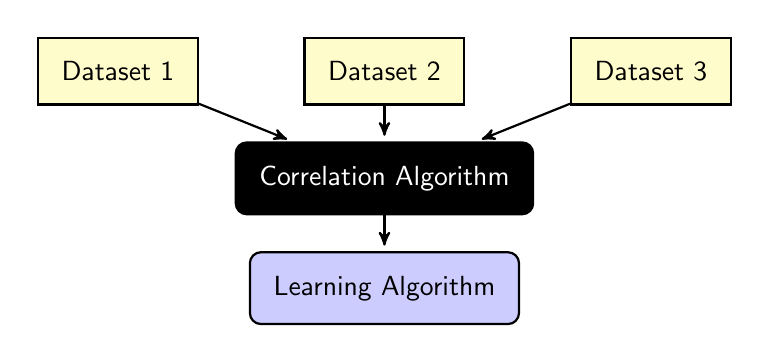
\begin{tikzpicture}[
      font=\sffamily,
      every matrix/.style={ampersand replacement=\&,column sep=3ex,row sep=3ex},
      dataset/.style={draw,thick,fill=yellow!20,inner sep=.3cm},
      sink/.style={dataset,rounded corners,fill=black, text=white},
      app/.style={dataset,rounded corners,fill=blue!20},
      dots/.style={gray,scale=2},
      to/.style={->,>=stealth',shorten >=2pt,thick,font=\sffamily\footnotesize},
      every node/.style={align=center}]

      \matrix{
        \node[dataset] (dataset1) {Dataset 1};
        \& \node[dataset] (dataset2) {Dataset 2};
        \& \node[dataset] (dataset3) {Dataset 3}; \\

        \& \node[sink] (blackbox) {Correlation Algorithm}; \& \\

        \& \node[app] (application) {Learning Algorithm}; \& \\      
      };

      \draw[to] (dataset1) -- (blackbox);
      \draw[to] (dataset2) -- (blackbox);
      \draw[to] (dataset3) -- (blackbox);
      \draw[to] (blackbox) -- (application);

    \end{tikzpicture}
  \end{center}

  \begin{center}
    \textbf{Thesis Goal}\\
    \vspace{1ex}
    \fcolorbox{black}[HTML]{F1F1F1}{\parbox{0.6\textwidth}{%
        \centering Develop theoretically justified, robust\\ correlation algorithms for\\
        multi-dataset fusion}}
  \end{center}

    
\end{frame}


%%%%%%%%%%%%%%%%%%%%%%%%%%%%%%%%%%%%%%%%%%%%%%%%%%%%%%%%%%%%%%%%%%%
\begin{frame}{Thesis Outline}

  \begin{enumerate}
  \item Introduction
  \item Performance of Matched Subspace Detectors Using Finite Training Data
  \item Extensions of Deterministic MSD to Missing Data and Useful Subspace Components
  \item Detection of Correlated Signals using CCA and ICCA
  \item Estimation of Canonical Vectors in CCA and ICCA
  \item Top Singular Values of Cross Covariance Matrices
  \item Signal Detection of Random Projections of Signal-Plus-Noise Matrices
  \item Correlation Based Methods for Detection and Regression
  \item Correlation Based Methods for Image Annotation
  \item Detection of Correlated Signals in More than Two Datasets
  \end{enumerate}

\end{frame}

%%%%%%%%%%%%%%%%%%%%%%%%%%%%%%%%%%%%%%%%%%%%%%%%%%%%%%%%%%%%%%%%%%%
\begin{frame}{Thesis Outline}
  \addtocounter{framenumber}{-1}
  \begin{enumerate}
  \item \textcolor{textlightgray}{Introduction}
  \item \textcolor{textlightgray}{Performance of Matched Subspace Detectors Using Finite
      Training Data} 
  \item \textcolor{textlightgray}{Extensions of Deterministic MSD to Missing Data and
      Useful Subspace Components} 
  \item {\color{textred}Detection of Correlated Signals using CCA and ICCA}
  \item \textcolor{textlightgray}{Estimation of Canonical Vectors in CCA and ICCA}
  \item \textcolor{textred}{Top Singular Values of Cross Covariance Matrices}
  \item \textcolor{textred}{Signal Detection of Random Projections of
      Signal-Plus-Noise Matrices} 
  \item \textcolor{textlightgray}{Correlation Based Methods for Detection and Regression} 
  \item \textcolor{textred}{Correlation Based Methods for Image Annotation}
  \item \textcolor{textred}{Detection of Correlated Signals in More than Two Datasets}
  \end{enumerate}

\end{frame}

%%%%%%%%%%%%%%%%%%%%%%%%%%%%%%%%%%%%%%%%%%%%%%%%%%%%%%%%%%%%%%%%%%%%%%%%%%%%%%%%%%%%%%%%%%
\begin{frame}{Two-Dataset Model}

  \begin{center}
    \textbf{Linear Subspace Model\\}
    \vspace{0.5ex}
    \fcolorbox{black}[HTML]{F1F1F1}{\parbox{0.4\textwidth}{%
        \be\ba
        & x_i = \Ux\sx+\zx\\
        & y_i = \Uy\sy+\zy\\
        \ea\ee
      }}
  \end{center}

  \textbf{Parameters}
  \begin{itemize}
  \item $\Ux^H\Ux = I_{\kx}$, $\Uy^H\Uy = I_{\ky}$
  \item $\zx\simiid\mathcal{CN}(0,I_p)$, \,\,\,$\zy\simiid\mathcal{CN}(0,I_q)$
  \item
    $\E{\left[\begin{array}{c}\sx\\ \sy\end{array}\right]\left[\begin{array}{cc} \sx^H
          & \sy^H \end{array}\right]}= \left[\begin{array}{cc}\Tx & \Kxy\\
        \Kxy^H & \Ty \end{array}\right]$
  \item $\Kxy = \Tx^{1/2}\Pxy\Ty^{1/2}$
  \item $\Theta_x =
    \diag\left(\left(\theta_1^{(x)}\right)^2,\dots,\left(\theta_{k_x}^{(x)}\right)^2\right)$,\,\,\,
    $\Theta_y    =
    \diag\left(\left(\theta_1^{(y)}\right)^2,\dots,\left(\theta_{k_y}^{(y)}\right)^2\right)$  
  \item $\Pxy$ contains correlations $\rho_{kj}$ between signals of $\xii$ and $\yii$
  \item $\widetilde{K}_{xy}
    =\left(\Theta_x+I_{k_x}\right)^{-1/2}K_{xy}\left(\Theta_y+I_{k_y}\right)^{-1/2}$, with
    singular values $\kappa_1,\dots,\kappa_{\min(k_x,k_y)}$
  \end{itemize}
\end{frame}

%%%%%%%%%%%%%%%%%%%%%%%%%%%%%%%%%%%%%%%%%%%%%%%%%%%%%%%%%%%%%%%%%%%%%%%%%%%%%%%%%%%%%%%%%%
\begin{frame}{Canonical Correlation Analysis}

  \textbf{What is it?}
  \begin{itemize}
  \item Dimensionality reduction algorithm for exactly 2 datasets
  \item Correlation coefficients, linear transformations
  \end{itemize}

  \vspace{1ex}

  \textbf{What is it not?}
  \begin{itemize}
  \item Data fusion algorithm
  \end{itemize}
 

  \vspace{1ex}

  \begin{columns}
    \begin{column}{0.35\textwidth}
      \textbf{Covariance matrices}
      \begin{itemize}
      \item $\Rxx = \E{x_ix_i^H}$
      \item $\Ryy = \E{y_iy_i^H}$
      \item $\Rxy = \E{x_iy_i^H}$
      \end{itemize}
    \end{column}
    \begin{column}{0.55\textwidth}
      \begin{center}
        \textbf{Optimization problem}
        \vspace{-1ex}
        \begin{empheq}[box={\mybluebox[5pt][5pt][boxgrey]}]{equation*}
          \begin{aligned}
            & \argmax_{w_x,w_y} &&\rho = w_x^HR_{xy}w_y\\
            & \text{subject to } && w_x^H\Rxx w_x=1\\
            &&&w_y^H\Ryy w_y = 1\\
          \end{aligned}
        \end{empheq}
     \end{center}
    \end{column}
  \end{columns}

  \vspace{1ex}

  \textbf{Variable Transformation}
  \begin{itemize}
  \item $f=\Rxx^{1/2}w_x$
  \item $g=\Ryy^{1/2}w_y$
  \end{itemize}

\end{frame}

%%%%%%%%%%%%%%%%%%%%%%%%%%%%%%%%%%%%%%%%%%%%%%%%%%%%%%%%%%%%%%%%%%%%%%%%%%%%%%%%%%%%%%%%%%
\begin{frame}{Canonical Correlation Analysis}
  \addtocounter{framenumber}{-1}
  \textbf{What is it?}
  \begin{itemize}
  \item Dimensionality reduction algorithm for exactly 2 datasets
  \item Correlation coefficients, linear transformations
  \end{itemize}

  \vspace{1ex}

  \textbf{What is it not?}
  \begin{itemize}
  \item Data fusion algorithm
  \end{itemize}
 

  \vspace{1ex}

  \begin{center}
    \textbf{Optimization problem}
    \vspace{-1ex}
    \begin{empheq}[box={\mybluebox[5pt][5pt][boxgrey]}]{equation*}
      \begin{aligned}
        & \argmax_{f,g} &&\rho = f^H\,\underbrace{R_{xx}^{-1/2}R_{xy}R_{yy}^{-1/2}}_{\Ccca}g\\
        & \text{subject to } && \|f\|_2=1\,,\,\|g\|_2=1\\
      \end{aligned}
    \end{empheq}
  \end{center}


  \vspace{3ex}

  \begin{columns}[t]
    \begin{column}{0.3\textwidth}
      \textbf{Canonical Vectors}
      \begin{itemize}
      \item $w_x = R_{xx}^{-1/2}f$
      \item $w_y = R_{yy}^{-1/2}g$
      \end{itemize}
    \end{column}
    \begin{column}{0.4\textwidth}
      \centering
      \textbf{Insight}\\[-3ex]
      \begin{empheq}[box={\mybluebox[5pt][5pt][boxgrey]}]{equation*}
        \text{\# correlated signals $=k=\rank(\Ccca)$}
      \end{empheq}

    \end{column}
  \end{columns}

\end{frame}

%%%%%%%%%%%%%%%%%%%%%%%%%%%%%%%%%%%%%%%%%%%%%%%%%%%%%%%%%%%%%%%%%%%%%%%%%%%%%%%%%
\begin{frame}{Empirical CCA}

  \begin{columns}[t]
    \begin{column}{0.5\textwidth}

      \textbf{Training Datasets}
      \begin{itemize}
        \itemsep=1ex
      \item $X=\left[x_1,\dots,x_n\right]$
      \item $Y=\left[y_1,\dots,y_n\right]$
      \end{itemize}
    \end{column}
    \begin{column}{0.5\textwidth}

      \textbf{Sample Covariance Matrices}
      \begin{itemize}
      \item $\Rxxhat=\frac{1}{n}XX^H$
      \item $\Ryyhat=\frac{1}{n}YY^H$
      \item $\Rxyhat=\frac{1}{n}XY^H$
      \end{itemize}
    \end{column}
  \end{columns}

  \vspace{1ex}

  \begin{center}
    \textbf{Estimate}\\
    \fcolorbox{black}[HTML]{F1F1F1}{\parbox{0.4\textwidth}{%
        \be\ba
        &\Cccahat &&= \Rxxhat^{-1/2}\Rxyhat\Ryyhat^{-1/2}\\
        &&&=\widehat{F}\widehat{K}\widehat{G}^H
        \ea\ee
      }}
  \end{center}

  \textbf{Questions}
  \begin{itemize}
  \item How to estimate $k$?
  \item When do $\widehat{\rho}_{\text{cca}}^{(i)}=\widehat{k}_i$ represent actual
    correlations?
  \item How accurate are $\widehat{w}_x^{(i)} = \Rxxhat^{-1/2}\widehat{f}_i$ and
    $\widehat{w}_y^{(i)}=\Ryyhat^{-1/2}\widehat{g}_i$?
  \item Can we do better?
  \end{itemize}

\end{frame}

%%%%%%%%%%%%%%%%%%%%%%%%%%%%%%%%%%%%%%%%%%%%%%%%%%%%%%%%%%%%%%%%%%%%%%%%%%%%%%%%%%%%%%%%%%
\begin{frame}{Statistical Test for CCA Correlations}

  \begin{center}
    \textbf{Estimate of \# of Correlated Signals }\\[1ex]
    \fcolorbox{black}[HTML]{F1F1F1}{\parbox{0.4\textwidth}{%
        \be
        \widehat{k}_{\text{cca}} = \sum_{i=1}^{\min(p,q)} \indicator_{\left\{\left(\widehat{\rho}_{\text{cca}}^{(i)}\right)^2 >\tau_{\text{cca}}^{\alpha}\right\}}
        \ee
      }}
  \end{center}

  \vspace{3ex}

  \begin{columns}[T]
    \begin{column}{0.6\textwidth}
      \textbf{Setting the threshold}
      \begin{itemize}
      \item $F_{\text{cca}}$ is the cdf of largest singular values of $\Cccahat$ in the
        null setting of no correlation
      \item $\tau_{\text{cca}}^{\alpha} = F_{\text{cca}}^{-1}(1-\alpha)$ 
      \item $\tau_{\text{cca}}^{\alpha} \approx \sigma_{n,p,q}\twc^{-1}(1-\alpha) + \mu_{n,p,q}$
      \end{itemize}
    \end{column}
    \begin{column}{0.4\textwidth} 
      \centering
      \textbf{Tracy-Widom Distribution}\\
      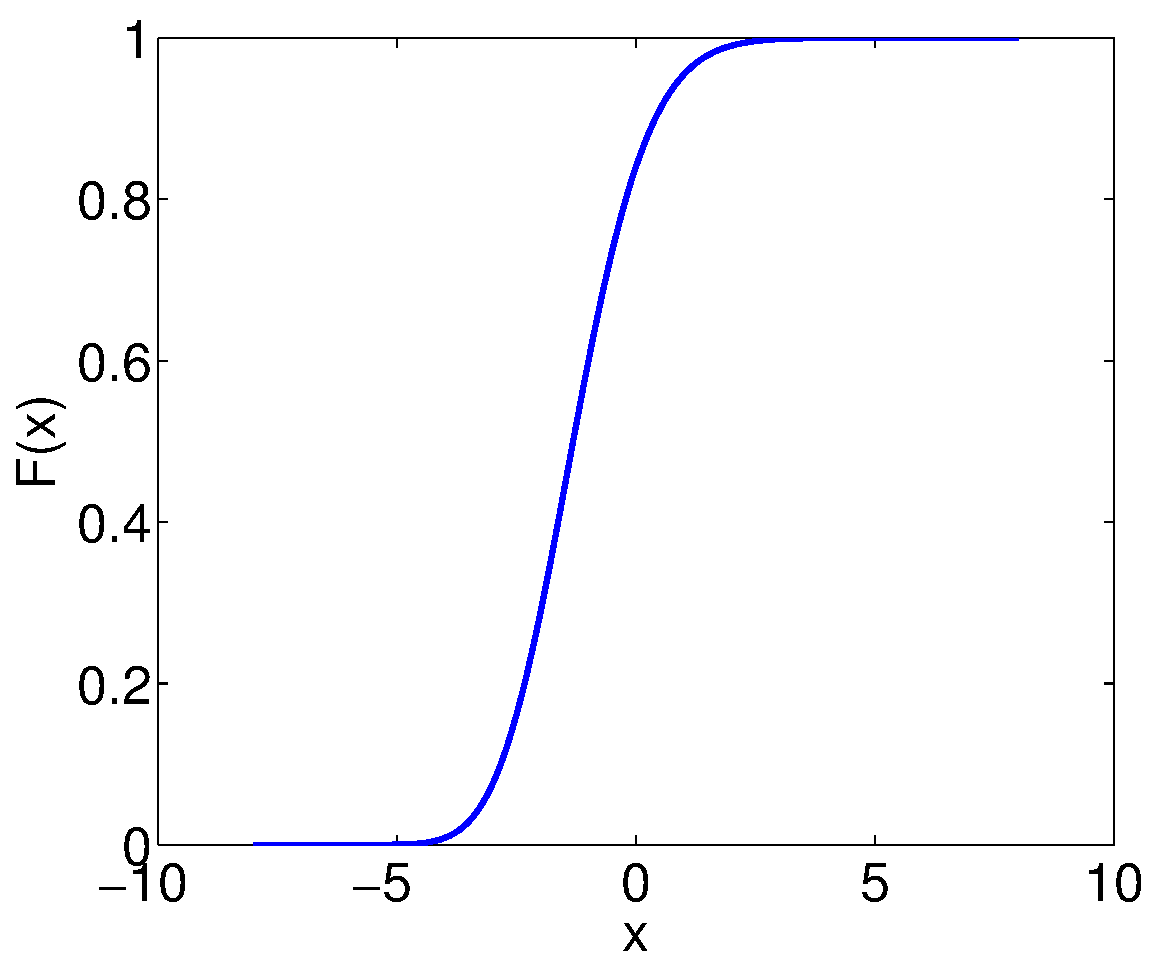
\includegraphics[width=\textwidth]{figures/tw.pdf}
    \end{column}
  \end{columns} 
\end{frame}


%%%%%%%%%%%%%%%%%%%%%%%%%%%%%%%%%%%%%%%%%%%%%%%%%%%%%%%%%%%%%%%%%%%%%%%%%%%%%%%%%%%%%%%%%%
\begin{frame}{Empirical CCA Consistency}

  \begin{Th}[Empirical CCA Consistency]\label{th:khat_lims}
    Let $p,q,n\to\infty$ with $p/n\to c_x$ and $q/n\to c_y$. Given the above linear subspace
    data model, 
    \be\ba
    & \widehat{k}_{\text{cca}} \convas k &&\text{ if } \kappa_k^2 >r_c \text{ and } n>p+q\\
    \ea\ee
    where
    \be
    r_c = \frac{c_xc_y+\sqrt{c_yc_y(1-c_x)(1-c_y)}}{(1-c_x)(1-c_y) + \sqrt{c_xc_y(1-c_x)(1-c_y)}}.
    \ee
  \end{Th}

  \vspace{3ex}

  \textbf{Recall}
  \begin{itemize}
  \item $\widetilde{K}_{xy}
    =\left(\Theta_x+I_{k_x}\right)^{-1/2}\Tx\Pxy\Ty\left(\Theta_y+I_{k_y}\right)^{-1/2}$
  \item Singular values $\kappa_1,\dots,\kappa_{\min(k_x,k_y)}$
  \end{itemize}

\end{frame}

%%%%%%%%%%%%%%%%%%%%%%%%%%%%%%%%%%%%%%%%%%%%%%%%%%%%%%%%%%%%%%%%%%%%%%%%%%%%%%%%
\begin{frame}{CCA Consistency}

  \textbf{Simulation parameters}
  \begin{itemize}
  \item $p=q=150$, $k=1$, $\theta_x=\theta_y$, $\alpha=0.01$
  \end{itemize}

  \vspace{1ex}

  \begin{center}  $\boldsymbol{\rho=}\mathbf{0.5}$\hspace{25ex}$\boldsymbol{\rho=0.9}$\\[0.5ex]
  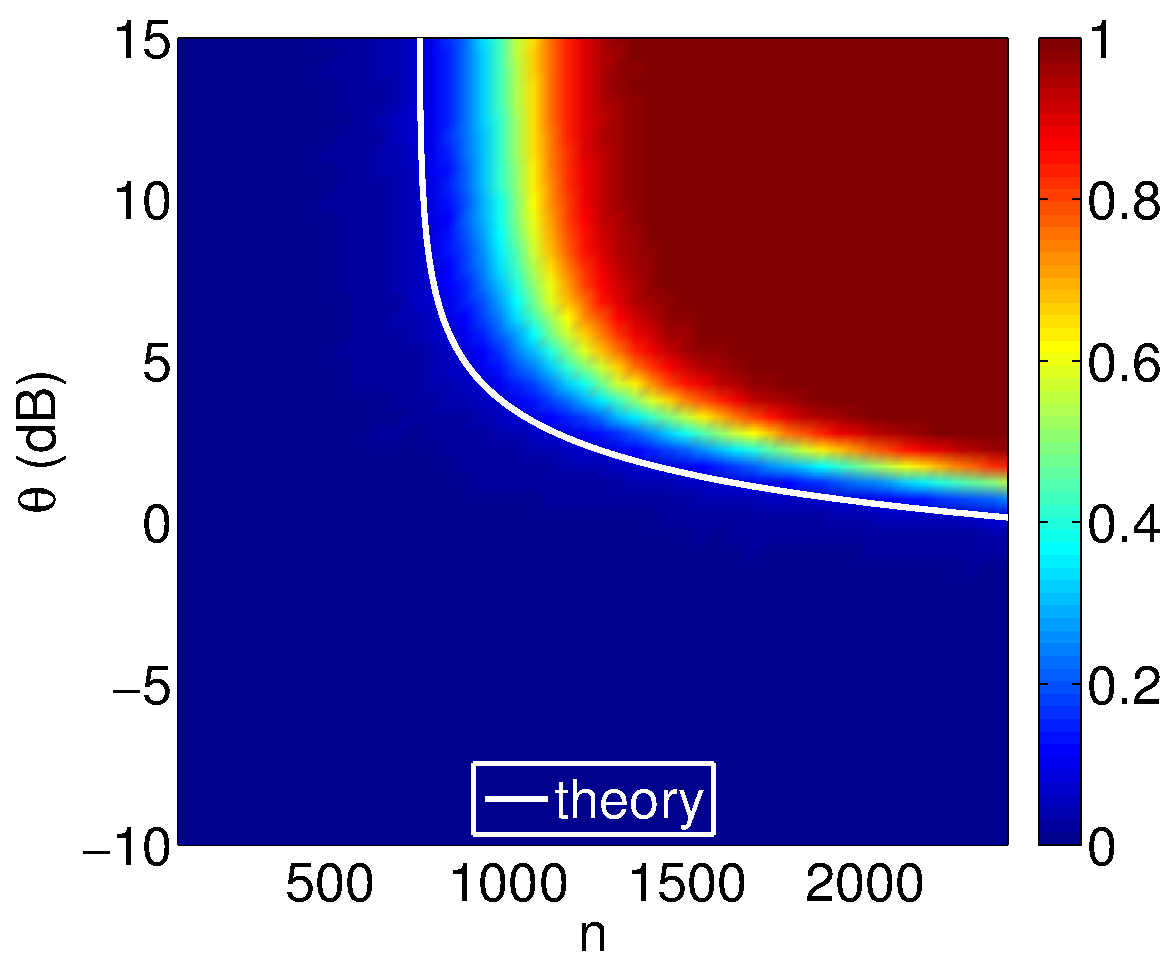
\includegraphics[width=0.4\textwidth]{figures/cca_rho5.pdf}\hspace{2ex}
  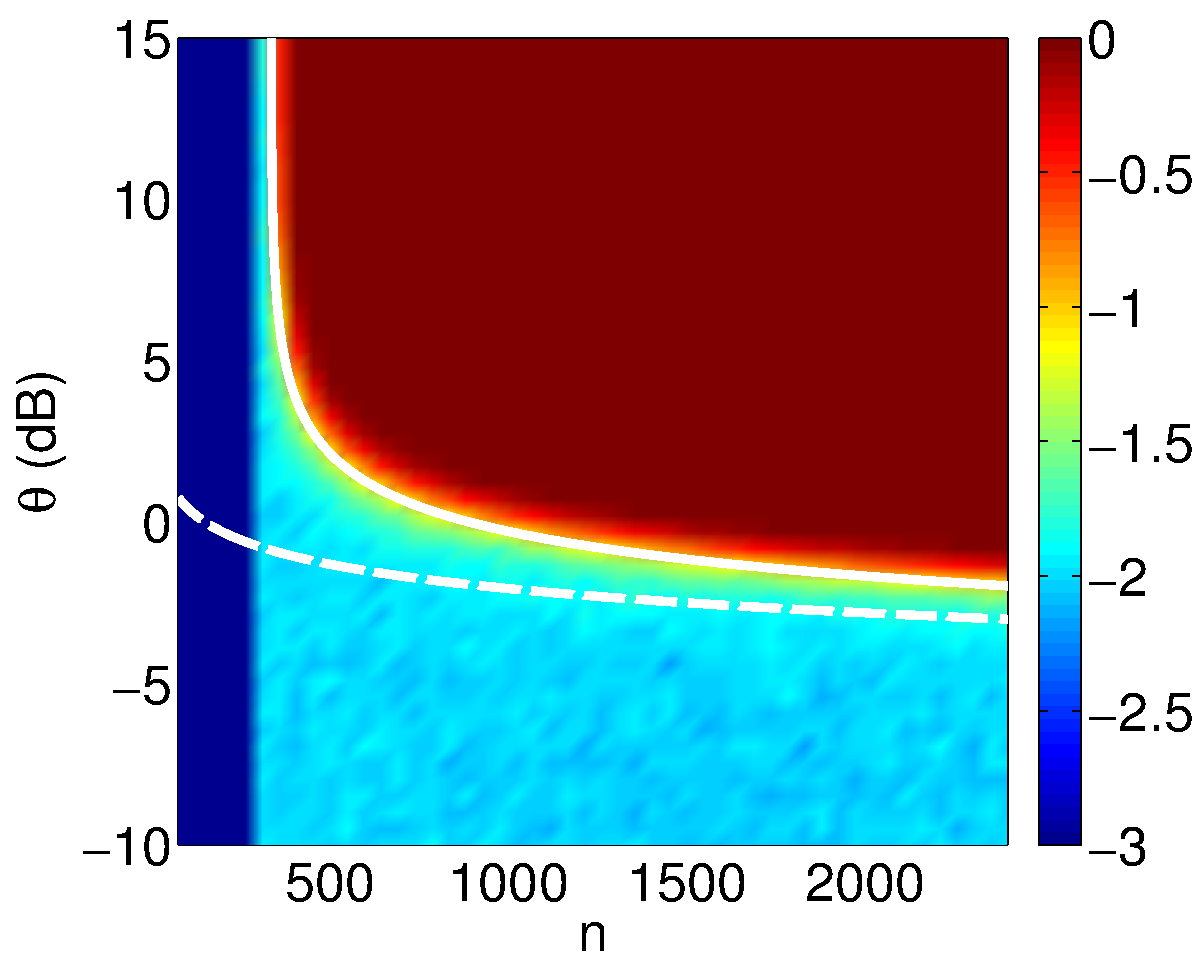
\includegraphics[width=0.4\textwidth]{figures/cca_rho9.pdf}
\end{center}



  
  \textbf{Problems!}
  \begin{itemize}
  \item Degenerate case when $n<p+q$ (Pezeshki 2004)
  \item Consistency boundary is dependent on correlation
  \end{itemize}

\end{frame}

%%%%%%%%%%%%%%%%%%%%%%%%%%%%%%%%%%%%%%%%%%%%
\begin{frame}{Informative CCA (ICCA)}

  \small

  \textbf{Not all singular vectors are informative!} (Nadakuditi, 2011)
  \begin{itemize}
  \item Trim data SVD's to only use informative components
  \end{itemize}

  \vspace{2ex}

  \fcolorbox{black}[HTML]{F1F1F1}{\parbox{0.9\textwidth}{%
  \begin{enumerate}
    \itemsep=1ex
  \item Trim data SVD's: $X=\widehat{U}_x\,\widehat{\Sigma}_x\,\widehat{V}_x^H$ and $Y=\widehat{U}_y\,\widehat{\Sigma}_y\, \widehat{V}_y^H$
    \begin{itemize}
    \item $\Uxcir = \widehat{U}_x\left(:\,,1:\widehat{k}_x\right)$, $\Uycir = \widehat{U}_y\left(:\,,1:\widehat{k}_y\right)$
    \item $\Vxcir = \widehat{V}_x\left(:\,,1:\widehat{k}_x\right)$, $\Vycir = \widehat{V}_y\left(:\,,1:\widehat{k}_y\right)$
    \end{itemize}

  \item Form
    $\Ciccahat=\Uxcir\Vxcir^H\Vycir\Uycir$
  \item Take SVD: $\Ciccahat = \widetilde{F}\widetilde{K}\widetilde{G}^H$
  \item $\widehat{\rho}_{\text{icca}}^{(i)} = \widetilde{k}_i$
  \item $\widetilde{w}_x^{(i)}=\widehat{R}_{xx}^{-1/2}\,\widetilde{f}_i$
  \item $\widetilde{w}_y^{(i)}=\widehat{R}_{yy}^{-1/2}\,\widetilde{g}_i$
  \end{enumerate}}}

\end{frame}

%%%%%%%%%%%%%%%%%%%%%%%%%%%%%%%%%%%%%%%%%%%%%%%%%%%%%%%%%%%%%%%%%%%%%%%%%%%%%%%%
\begin{frame}{Statistical Test for ICCA Correlations}


  \begin{center}
    \textbf{Estimate of \# of Correlated Signals }\\[1ex]
    \fcolorbox{black}[HTML]{F1F1F1}{\parbox{0.4\textwidth}{%
        \be
        \widehat{k}_{\text{icca}} = \sum_{i=1}^{\min(\widehat{k}_x,\widehat{k}_y)} \indicator_{\left\{\left(\widehat{\rho}_{\text{icca}}^{(i)}\right)^2 >\tau_{\text{icca}}^{\alpha}\right\}}
        \ee
      }}
  \end{center}

  \textbf{Setting the threshold}
  \begin{itemize}
  \item $F_{\text{icca}}$ is the cdf of largest singular values of $\Ciccahat$ in the null setting
    of no correlation
  \item $\tau_{\text{icca}}^{\alpha} = F_{\text{icca}}^{-1}(1-\alpha)$ 
  \item $\tau_{\text{icca}}^{\alpha} \approx \sigma_{n,\kxhat,\kyhat}\twc^{-1}(1-\alpha) + \mu_{n,\kxhat,\kyhat}$
  \end{itemize}


  \begin{Th}[ICCA Consistency]\label{th:khat_lims}
    Let $p,q,n\to\infty$ with $p/n\to c_x$ and $q/n\to c_y$. Given the linear subspace
    data model, 
    \be\ba
    & \widehat{k}_{\text{icca}} \convas k && \text{ if } \min_{i=1,\dots,k_x} \theta_i^{(x)}>c_x^{1/4} \text{ and }
    \min_{i=1,\dots,k_y} \theta_i^{(y)}>c_y^{1/4} 
    \ea\ee
  \end{Th}
\end{frame}

%%%%%%%%%%%%%%%%%%%%%%%%%%%%%%%%%%%%%%%%%%%%%%%%%%%%%%%%%%%%%%%%%%%%%%%%%%%%%%%%
\begin{frame}{CCA and ICCA Consistency}
  \begin{itemize}
  \item $p=q=150$, $k=1$, $\theta_x=\theta_y$,$\alpha=0.01$
  \end{itemize}

  \begin{columns}[T]
  \begin{column}{0.01\textwidth}
    \vspace{15ex}
    \textbf{ CCA}\\
    \vspace{20ex}
    \textbf{ICCA}
  \end{column}
  \begin{column}{1\textwidth}
    \begin{center}
      $\boldsymbol{\rho=}\mathbf{0.5}$\hspace{25ex}$\boldsymbol{\rho=0.9}$\\[0.5ex]

        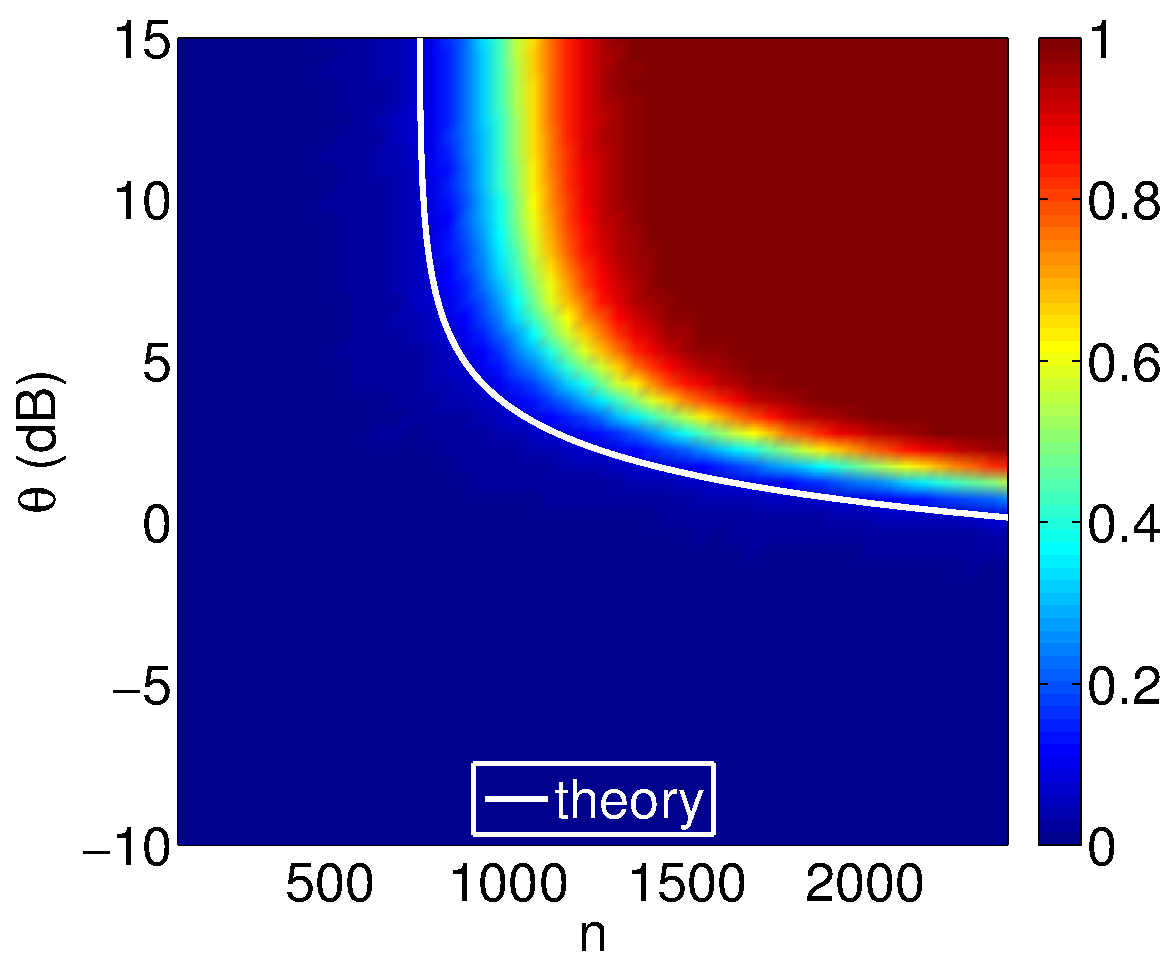
\includegraphics[width=0.35\textwidth]{figures/cca_rho5.pdf}\hspace{2ex}
        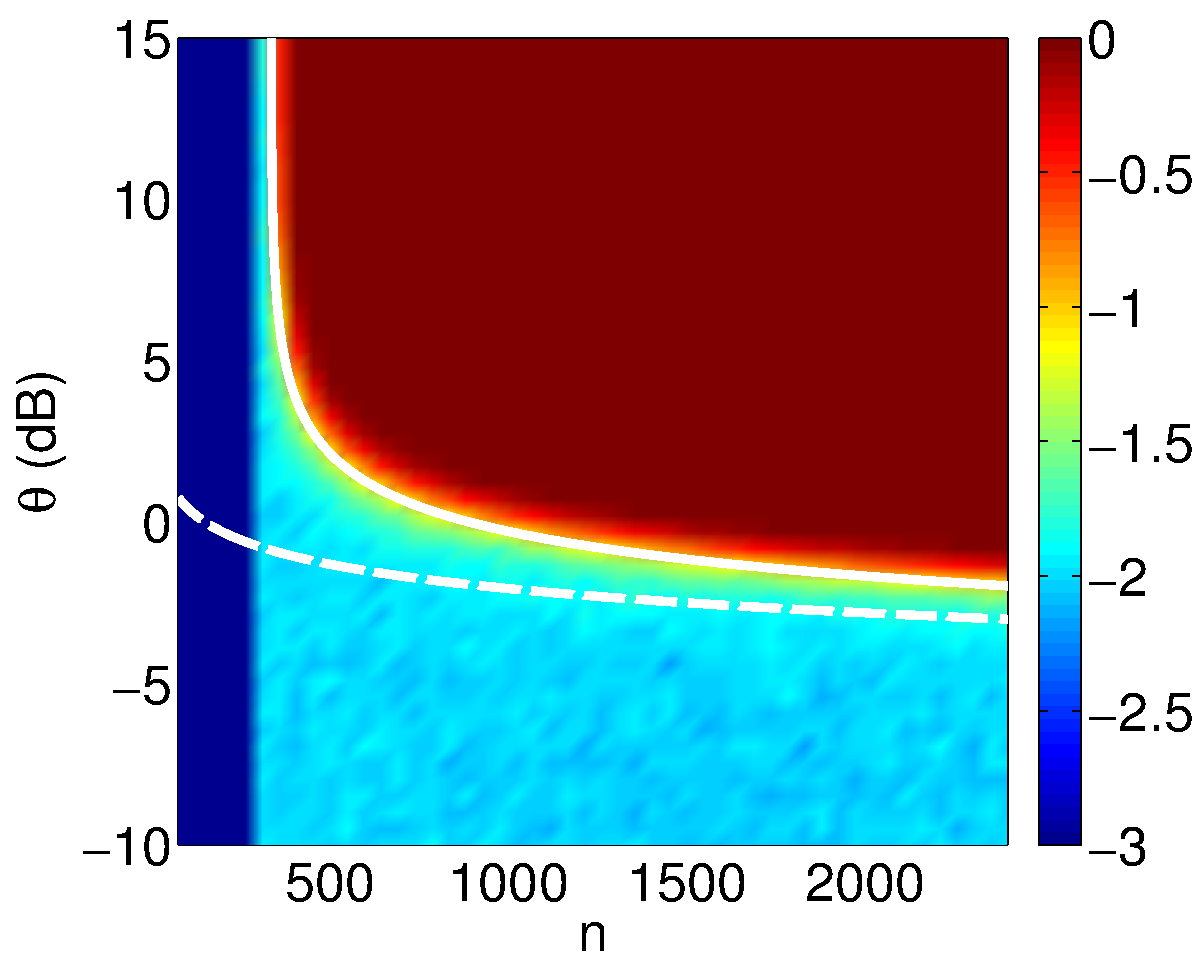
\includegraphics[width=0.35\textwidth]{figures/cca_rho9.pdf}\\[2ex]
        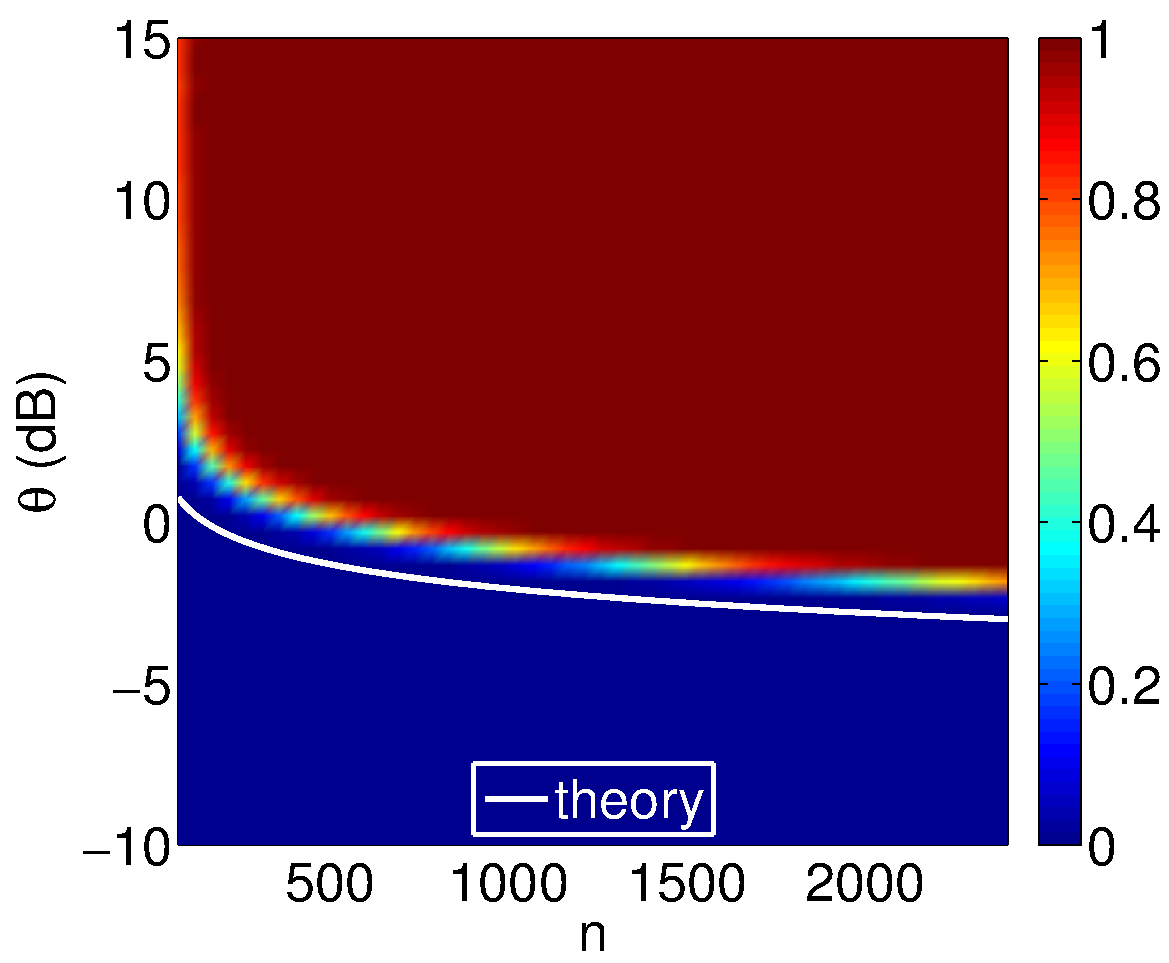
\includegraphics[width=0.35\textwidth]{figures/icca_rho5.pdf}\hspace{2ex}
        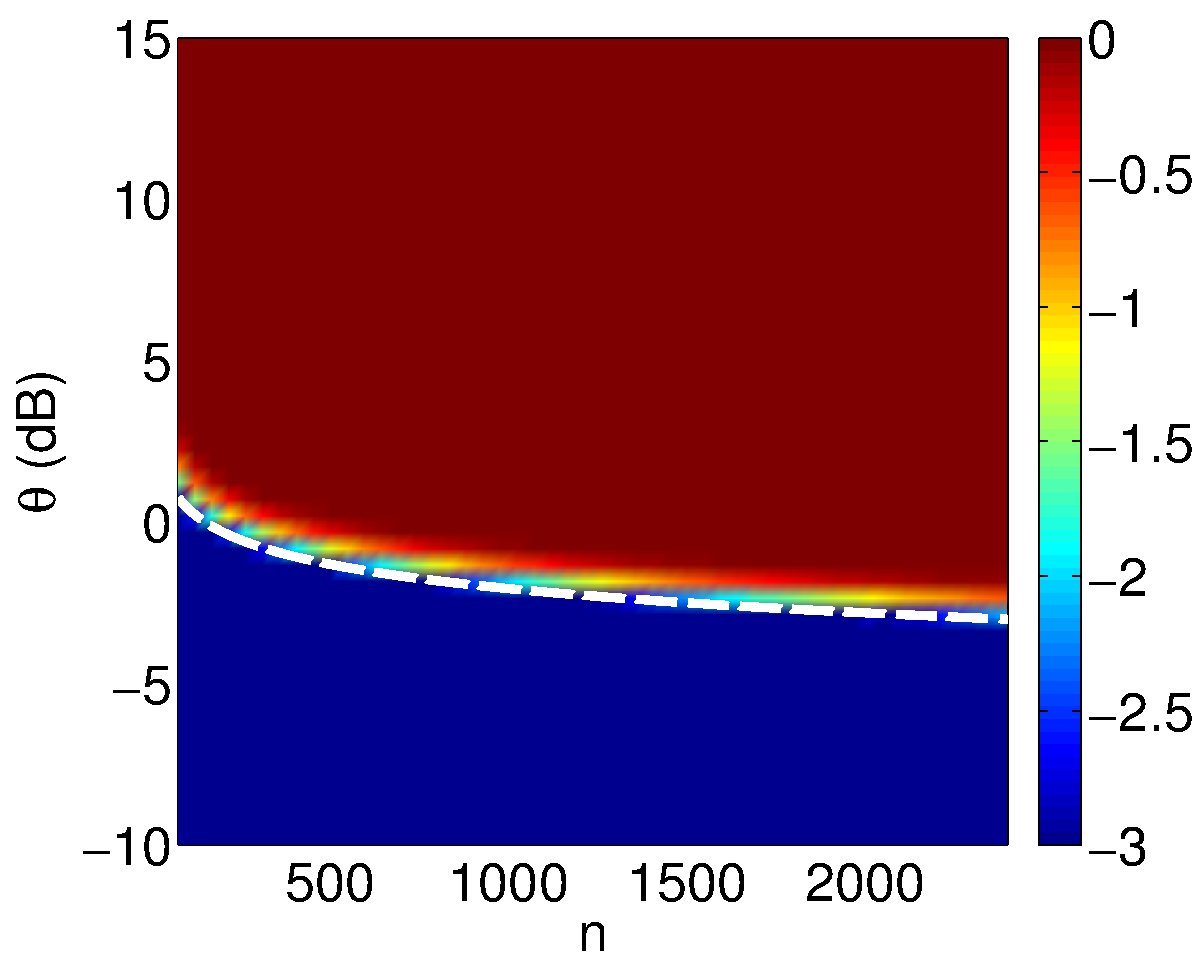
\includegraphics[width=0.35\textwidth]{figures/icca_rho9.pdf}
    \end{center}

  \end{column}
  \end{columns}



\end{frame}



%%%%%%%%%%%%%%%%%%%%%%%%%%%%%%%%%%%%%%%%%%%%%
\begin{frame}{CCA and ICCA Demonstration}

  \begin{itemize}
  \item Two-Camera flashing light demonstration
  \item Audio-Video demonstration
  \item Audio-Audio demonstration
  \end{itemize}

\end{frame}


%%%%%%%%%%%%%%%%%%%%%%%%%%%%%%%%%%%%%%%%%%%%%
\begin{frame}{CCA and ICCA Demonstration}
%      \textbf{ICCA Correlations}\hspace{20ex}\textbf{Significance}
    \begin{center}
      \hspace{2ex}\textbf{Video-Video}\hspace{14ex}\textbf{Audio-Video}\hspace{14ex}\textbf{Audio-Audio}
        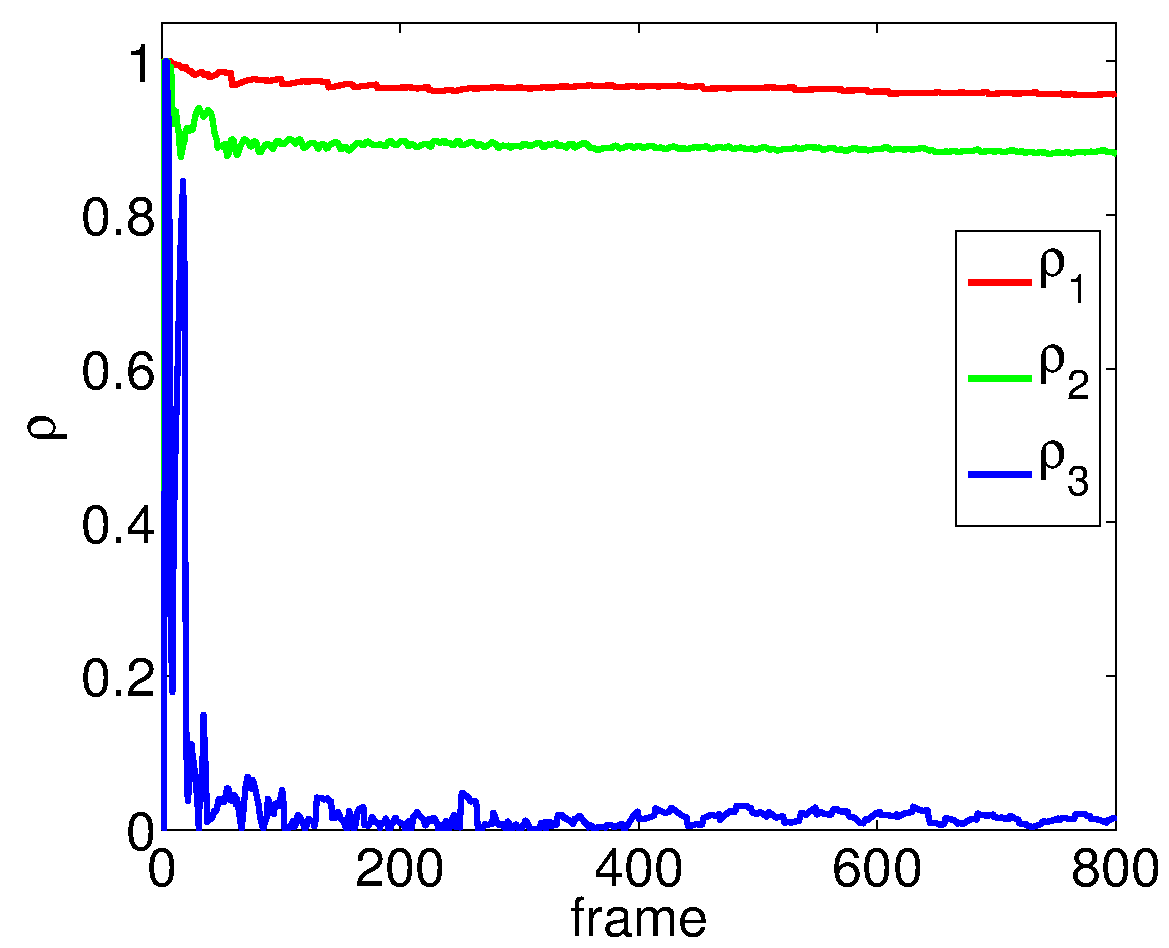
\includegraphics[width=0.3\textwidth]{figures/flashing_icca_corrs.pdf}
        \hspace{2ex}
        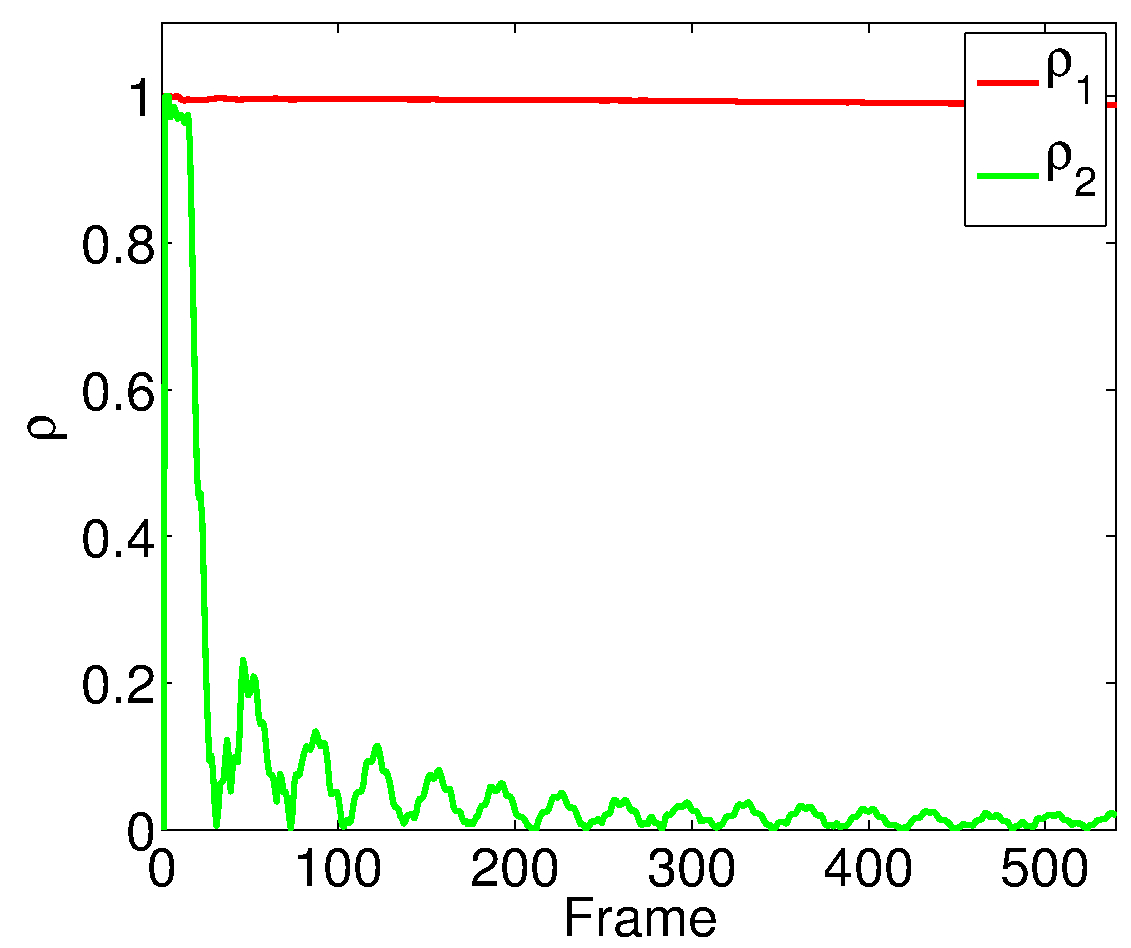
\includegraphics[width=0.3\textwidth]{figures/av_icca_corrs.pdf}
        \hspace{2ex}
        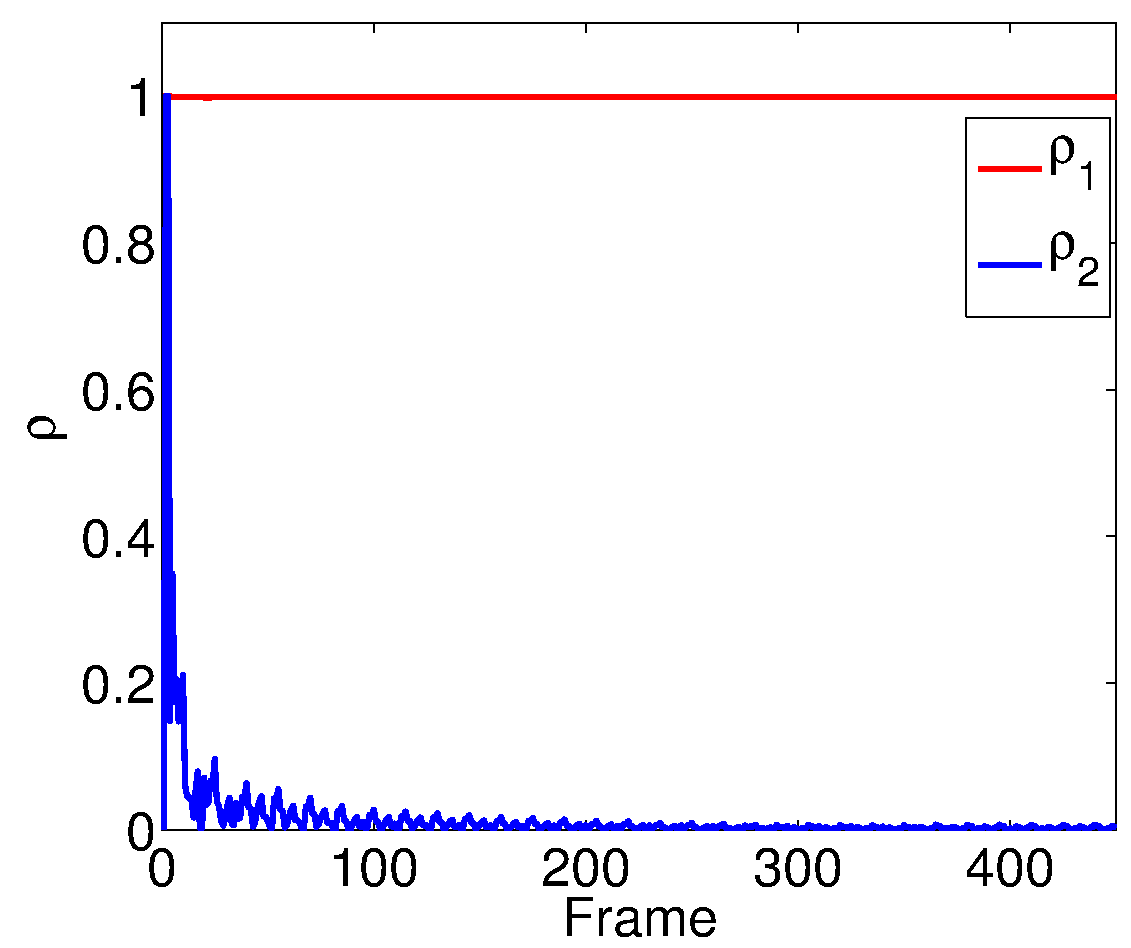
\includegraphics[width=0.3\textwidth]{figures/aa_icca_corrs.pdf}\\
        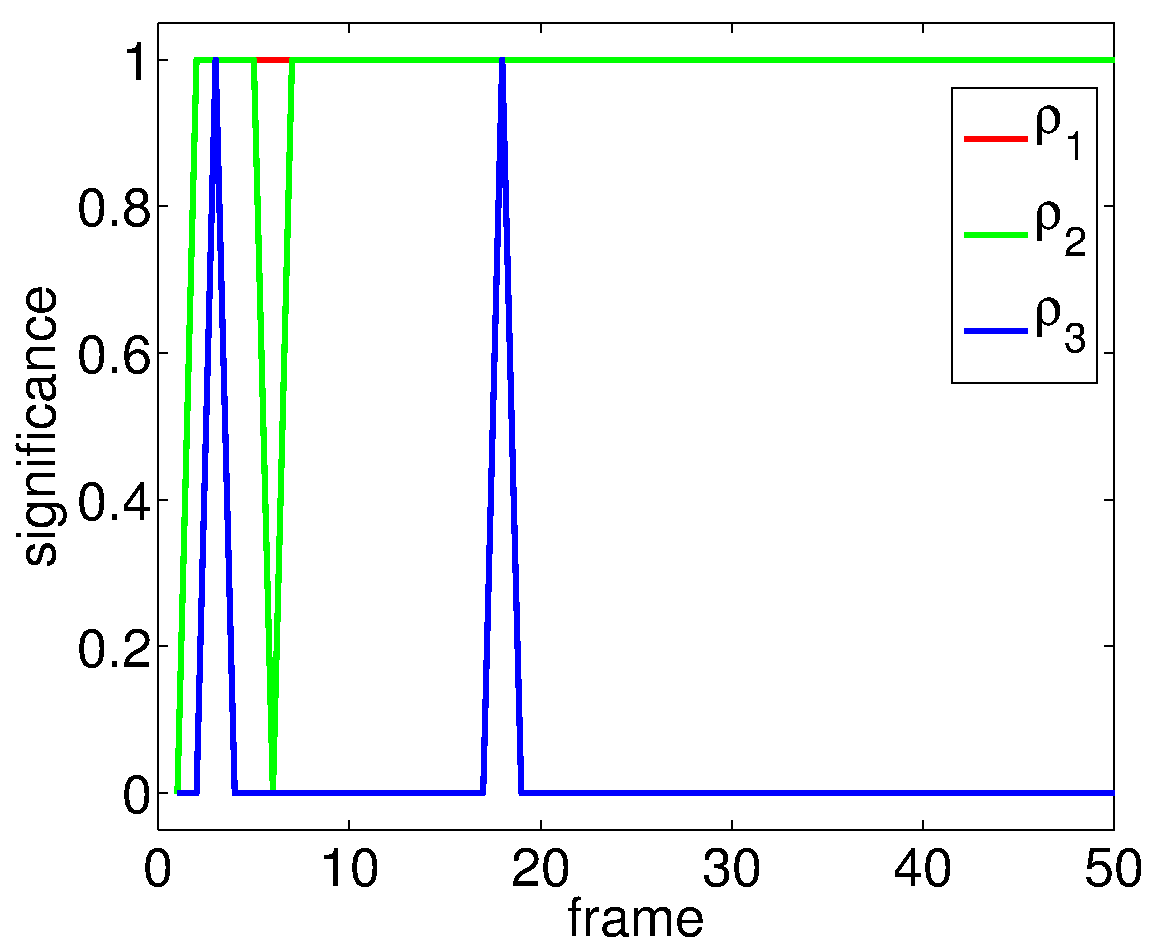
\includegraphics[width=0.3\textwidth]{figures/flashing_icca_sig_zoom.pdf}
        \hspace{2ex}
        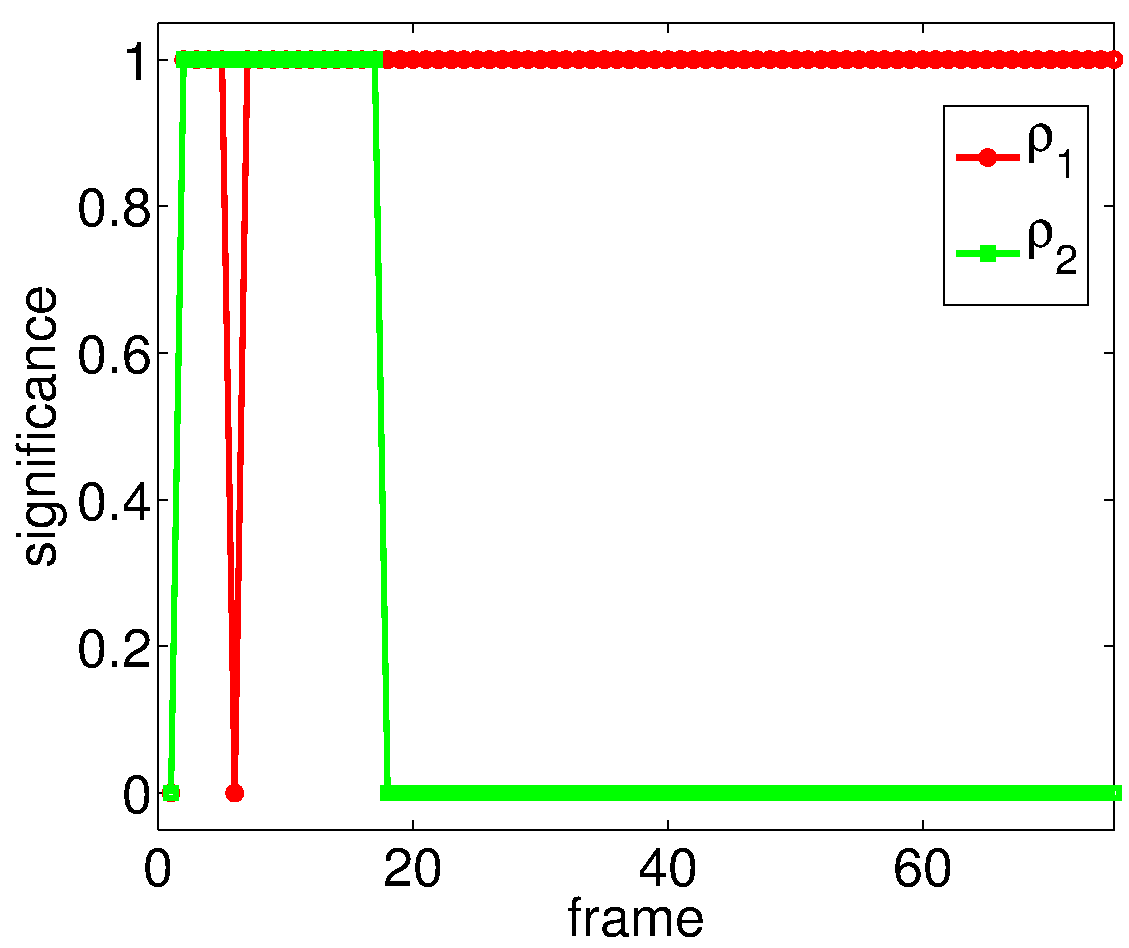
\includegraphics[width=0.3\textwidth]{figures/av_icca_sig_zoom.pdf}
        \hspace{2ex}
        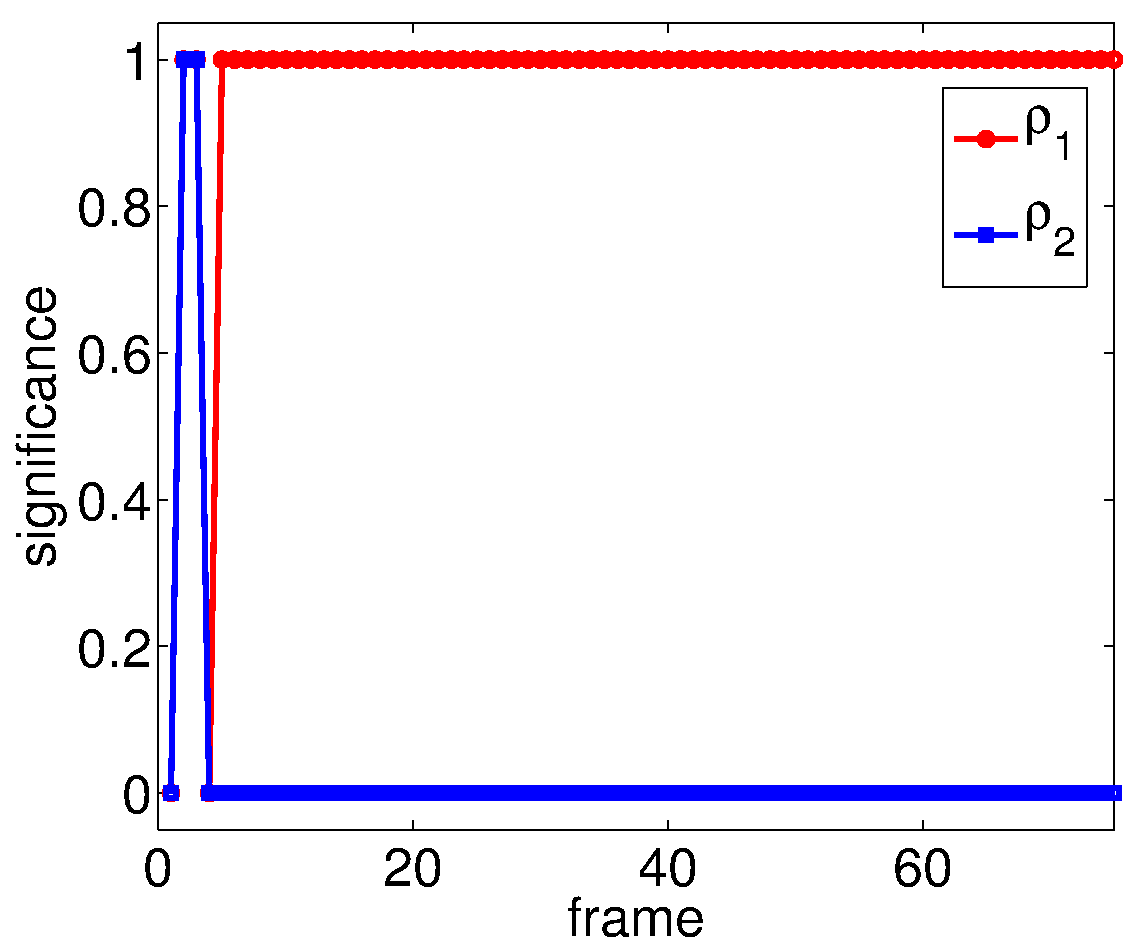
\includegraphics[width=0.3\textwidth]{figures/aa_icca_sig_zoom.pdf}
    \end{center}

\end{frame}

\begin{frame}{Missing Data Model}

\textbf{Matrix model}
\begin{itemize}
\item $V_x = \left[s_{x,1},\dots,s_{x,n}\right]$, $V_y = \left[s_{y,1},\dots,s_{y,n}\right]$
\item $Z_x = \left[z_{x,1},\dots,z_{x,n}\right]$, $Z_y = \left[z_{y,1},\dots,z_{y,n}\right]$
\end{itemize}

\vspace{2ex}

\begin{center}
\fcolorbox{black}[HTML]{F1F1F1}{\parbox{0.5\textwidth}{
    \be\ba
    & X = \left(U_xV_x^H + Z_x\right)\odot M_x\\
    & Y = \left(U_yV_y^H + Z_y\right)\odot M_y\\
    \ea\ee
  }}
\end{center}

\be\ba
& M^x_{ij} = \begin{cases} 1 & \text{ with probability } \gamma_x\\ 0 & \text{ with
    probability } 1-\gamma_x \end{cases}
& M^y_{ij} = \begin{cases} 1 & \text{ with probability } \gamma_y\\ 0 & \text{ with
    probability } 1-\gamma_y \end{cases}
\ea\ee
\begin{itemize}
\item $\odot$ denotes the Hadamard or element-wise product.
\end{itemize}
\end{frame}

\begin{frame}{CCA and ICCA Consistency in Missing Data}

\begin{Th}[Missing data consistency]\label{th:missing_data}
Let $p,q,n\to\infty$ with $p/n\to c_x$ and $q/n\to c_y$ and assume a low-coherence
condition on the signal vectors. Given a linear subspace data model with missing data
entries, 
\be\ba
& \widehat{k}_{\text{cca}} \convas k &&\text{ if } \min_{i=1,\dots,k}\kapcir_i^2 >r_c \text{ and } n>p+q\\
& \widehat{k}_{\text{icca}} \convas k && \text{ if } \min_{i=1,\dots,\widehat{k}_x}
\theta_i^{(x)}>\frac{c_x^{1/4}}{\sqrt{\gamma_x}} \text{ and } 
\min_{i=1,\dots,\widehat{k}_y} \theta_i^{(y)}>\frac{c_y^{1/4}}{\sqrt{\gamma_y}}
\ea\ee
where $\kapcir_i$ are the singular values of 
\be
\left(\gamma_x\Theta_x+I_{k_x}\right)^{-1/2}\left(\gamma_x\Theta_x\right)^{1/2}P_{xy}\left(\gamma_y\Theta_y\right)^{1/2}
\left(\gamma_y\Theta_y+I_{k_y}\right)^{-1/2}.
\ee
\end{Th}

\end{frame}

%%%%%%%%%%%%%%%%%%%%%%%%%%%%%%%%%%%%%%%%%%%%%%%%%%%%%%%%%%%%%%%%%%%%%%%%%%%%
\begin{frame}{CCA and ICCA Consistency in Missing Data}

  \begin{itemize}
  \item $p=q=150$, $k=1$, $\theta_x=\theta_y$,$\alpha=0.01$
  \end{itemize}

\setcounter{subfigure}{0}
\begin{figure}
  \begin{center}
    \subfigure[CCA $\rho=0.5$,$n=1200$]{
      \label{fig:cca_rho3_75}
      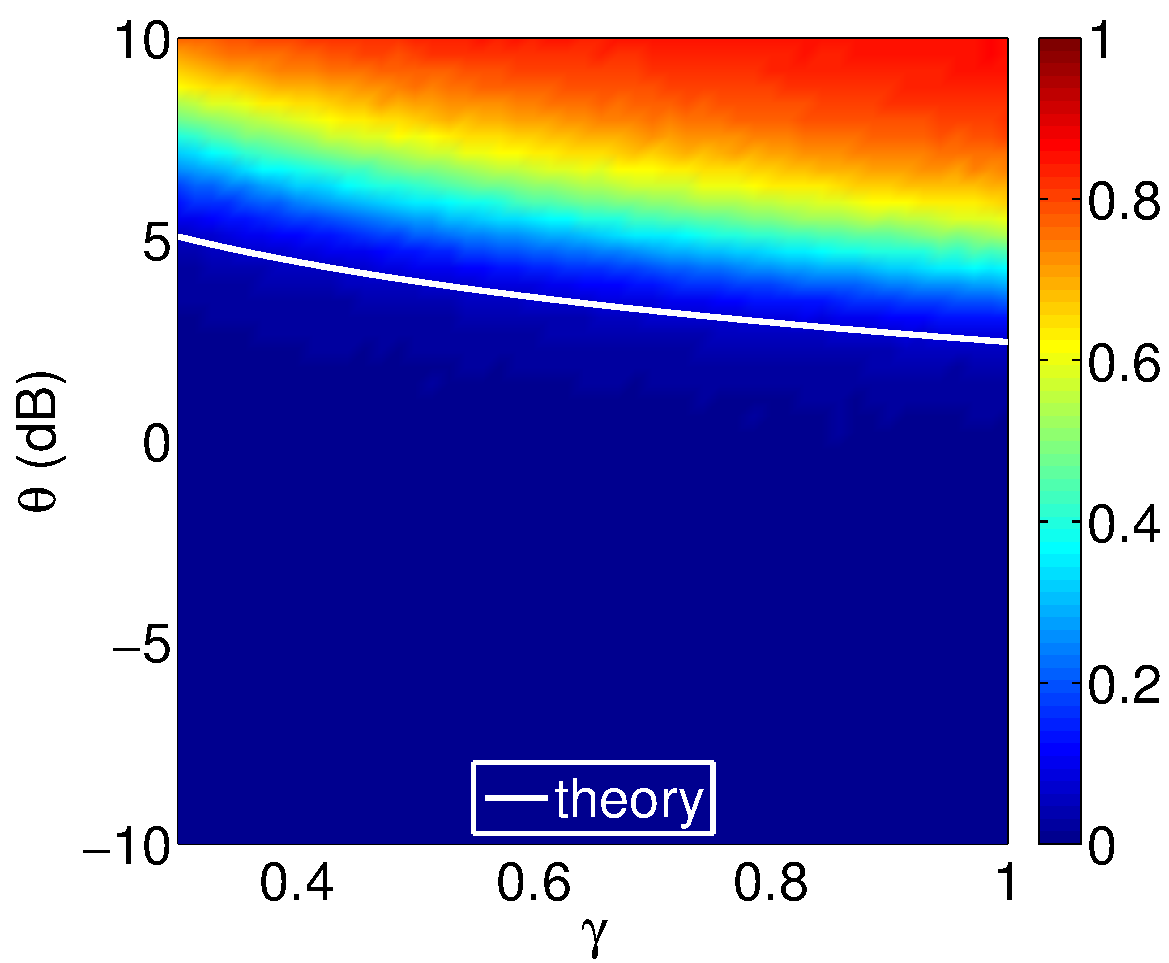
\includegraphics[width=0.35\textwidth]{figures/cca_missing_5_1200.pdf}
    }
    \subfigure[CCA $\rho=0.9$,$n=1200$]{
      \label{fig:cca_rho5_75}
      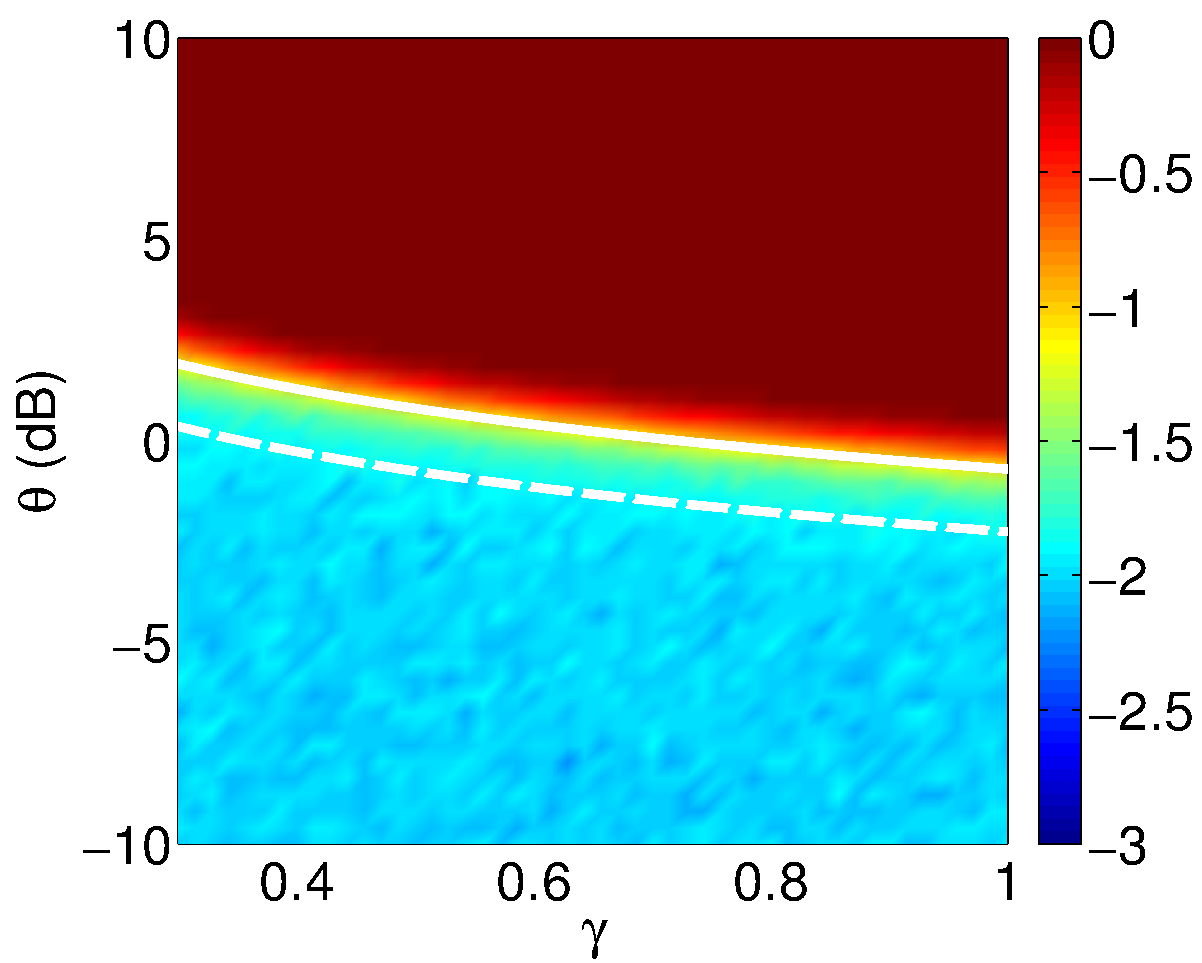
\includegraphics[width=0.35\textwidth]{figures/cca_missing_9_1200.pdf}
    }
    \subfigure[ICCA $\rho=0.5$, $n=1200$]{
      \label{fig:cca_rho7_75}
      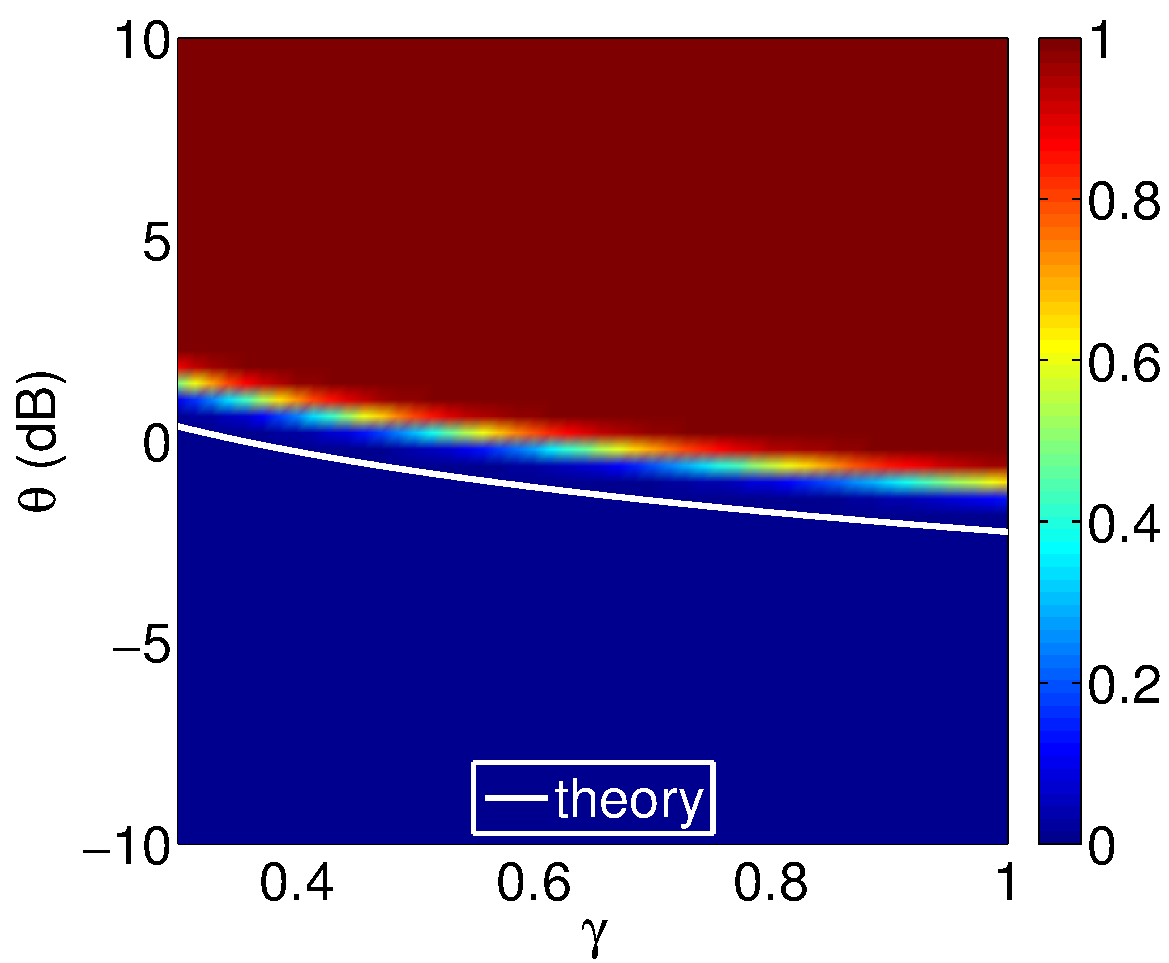
\includegraphics[width=0.35\textwidth]{figures/icca_missing_5_1200.pdf}
    }
    \subfigure[ICCA $\rho=0.9$, $n=1200$]{
      \label{fig:cca_rho9_75}
      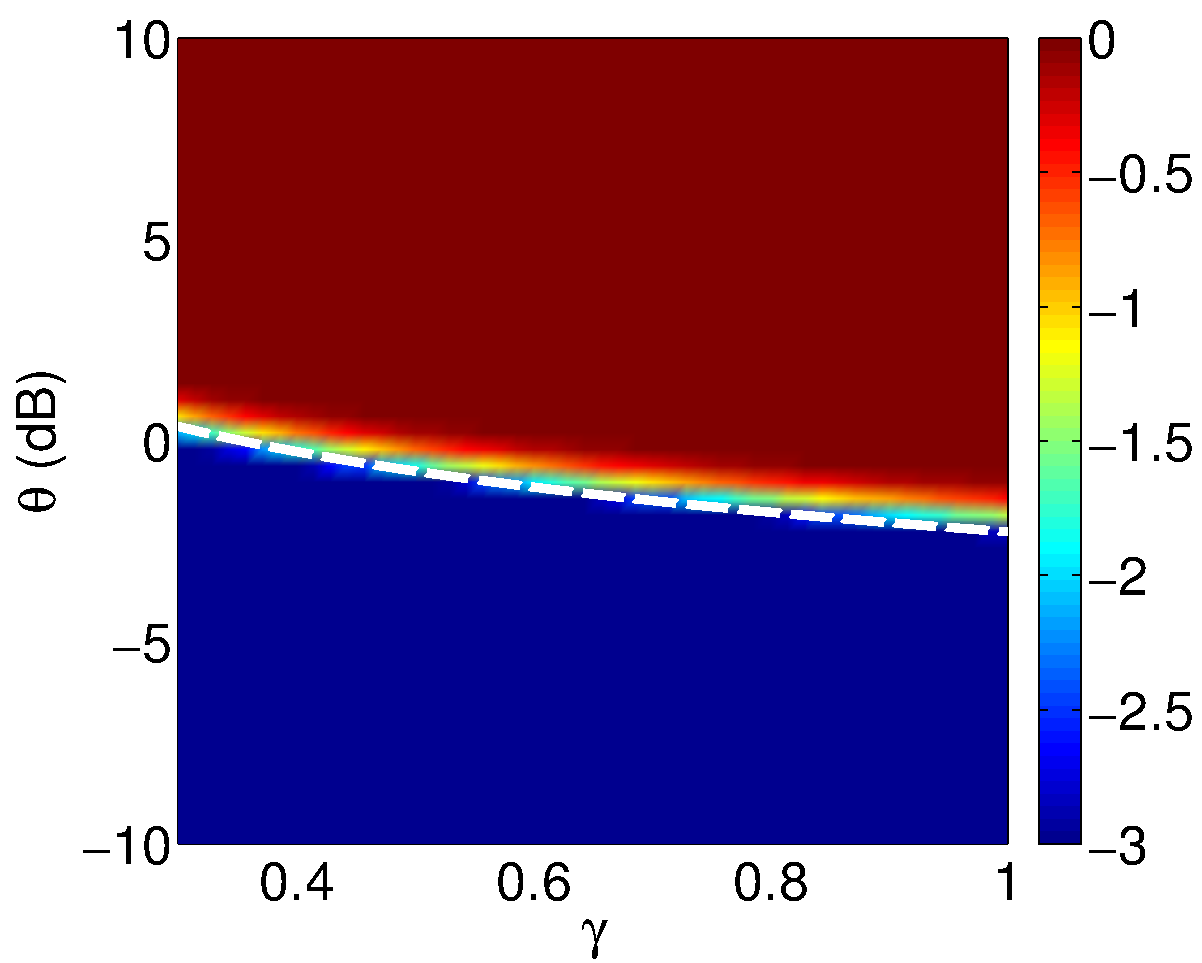
\includegraphics[width=0.35\textwidth]{figures/icca_missing_9_1200.pdf}
    }   
  \end{center}
\end{figure}

\end{frame}

%%%%%%%%%%%%%%%%%%%%%%%%%%%%%%%%%%%%%%%%%%%%%
\begin{frame}{Regularized CCA (RCCA)}
  \centering\textbf{Optimization problem}
  \vspace{-1ex}
  \begin{empheq}[box={\mybluebox[5pt][5pt][boxgrey]}]{equation*}
    \begin{aligned}
      & \argmax_{w_x,w_y} &&\rho = w_x^H\, R_{xy} w_y\\
      & \text{subject to } && w_x^H\,R_{xx} w_x + \eta \|w_x\|_2^2\leq1\\
      &&& w_y^H\,R_{yy}w_y+\eta \|w_y\|_2^2\leq1\\
    \end{aligned}
  \end{empheq}

  \vspace{2ex}

  \centering\textbf{SVD Solution}
  \vspace{-1ex}
  \begin{empheq}[box={\mybluebox[5pt][5pt][boxgrey]}]{equation*}
    \begin{aligned}
    &\widehat{C}_{\text{reg}} &&= \left(\widehat{R}_{xx}+\eta
      I_{p}\right)^{-1/2}\widehat{R}_{xy}\left(\widehat{R}_{yy}+\eta
      I_{q}\right)^{-1/2}\\
    \end{aligned}
  \end{empheq}

\end{frame}


%%%%%%%%%%%%%%%%%%%%%%%%%%%%%%%%%%%%%%%%%%%%%
\begin{frame}{Limit of RCCA}

\begin{itemize}
\item AUC for signal vs. noise, $k=1$, $p=100$, $q=150$, $\rho=0.9$
\end{itemize}


  \setcounter{subfigure}{0}
  \begin{figure}
    \begin{center}
      \subfigure[$\eta=0.0001$]{       
        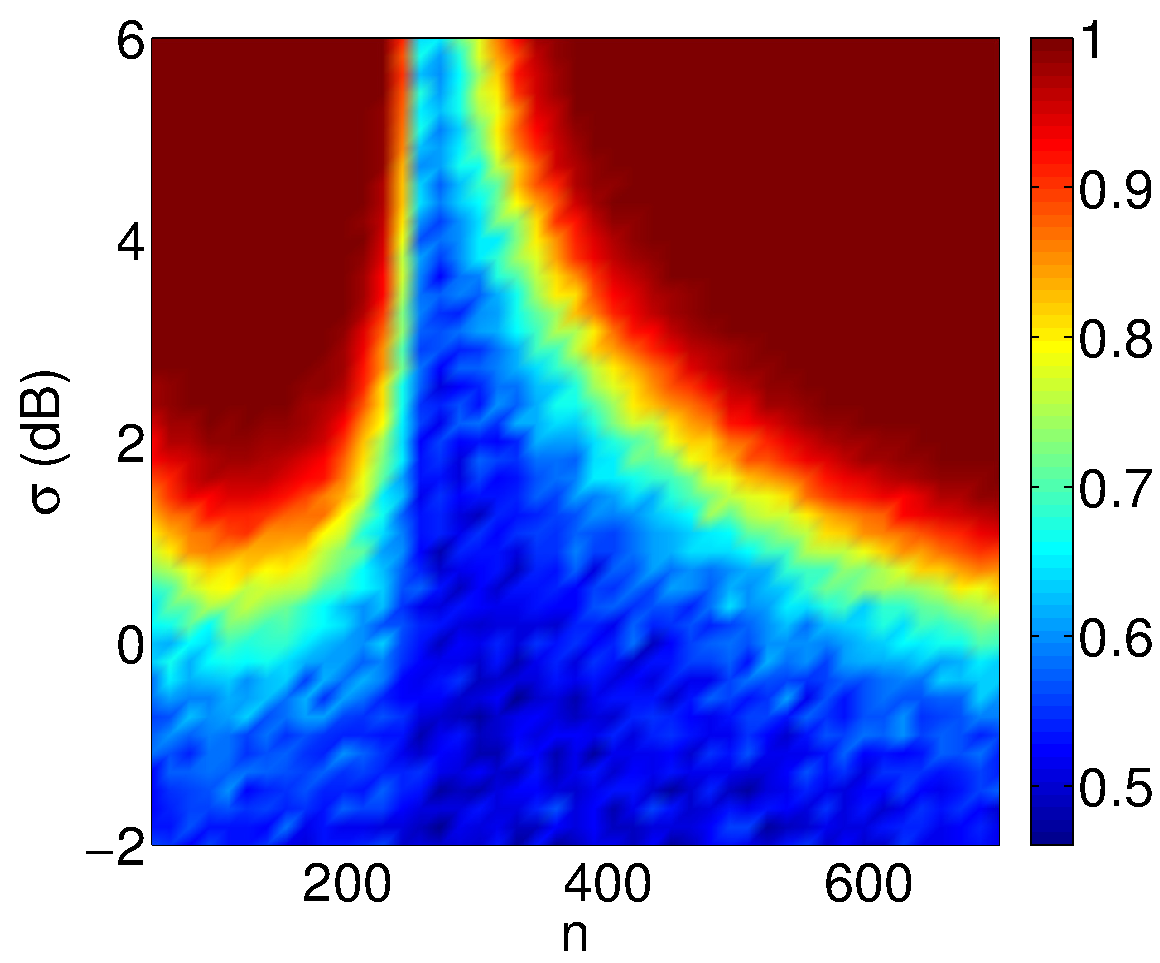
\includegraphics[width=0.35\textwidth]{figures/eta1_auc.pdf}
      }
      \subfigure[$\eta=0.01$]{       
        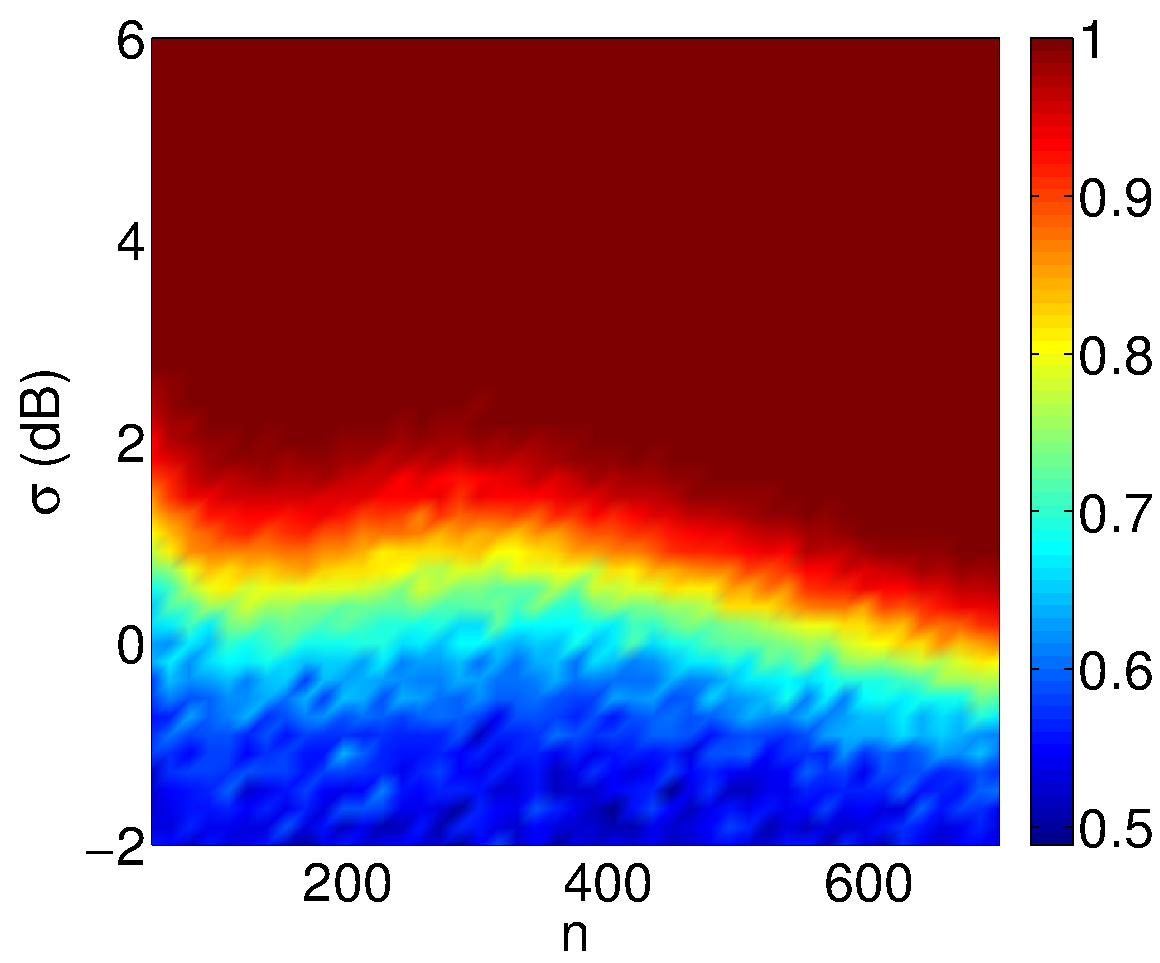
\includegraphics[width=0.35\textwidth]{figures/eta2_auc.pdf}
      }
      \subfigure[$\eta=10$]{       
        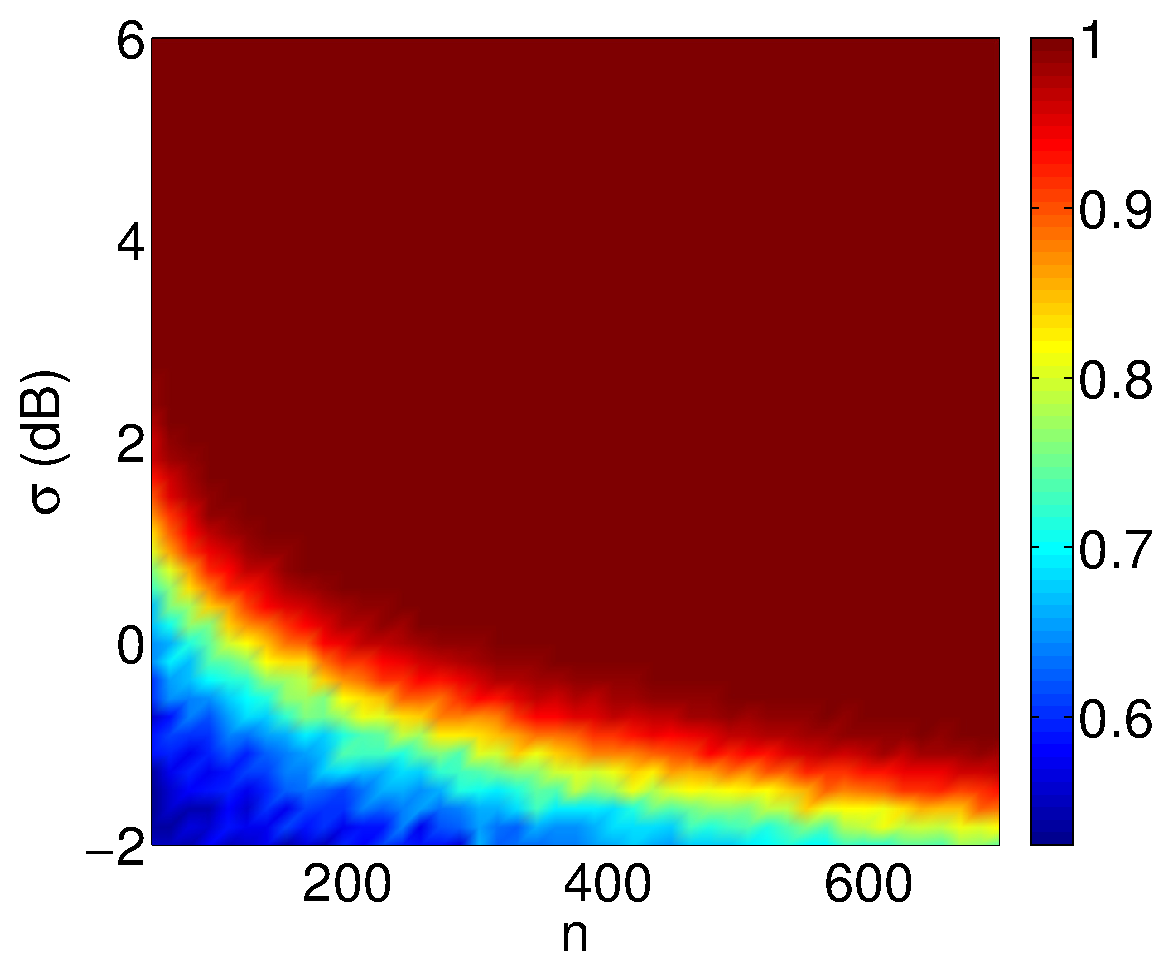
\includegraphics[width=0.35\textwidth]{figures/eta3_auc.pdf}
      }
      \subfigure[$\eta=1000$]{
        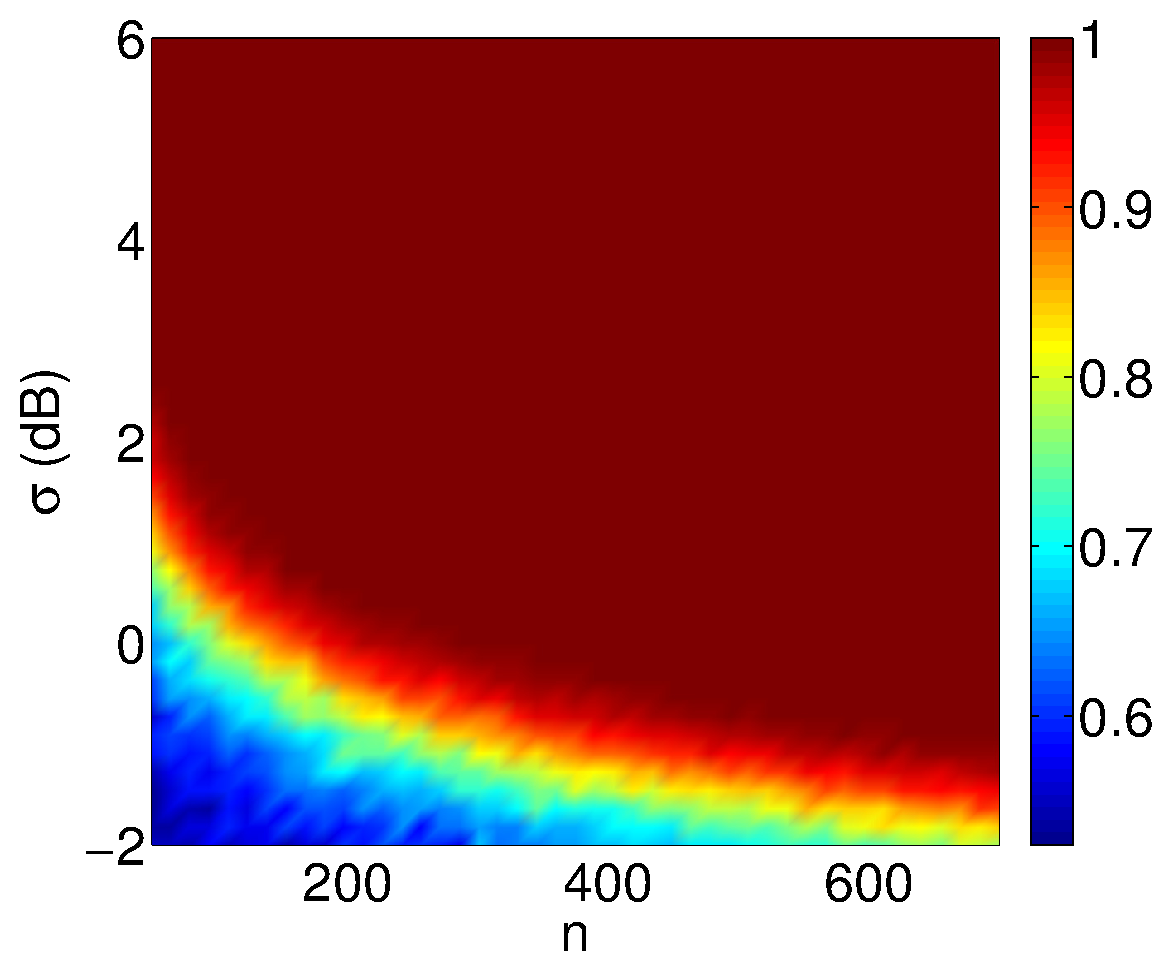
\includegraphics[width=0.35\textwidth]{figures/eta4_auc.pdf}
      }
    \end{center}
  \end{figure}

\end{frame}

%%%%%%%%%%%%%%%%%%%%%%%%%%%%%%%%%%%%%%%%%%%%%
\begin{frame}{Limit of RCCA}

  \begin{Th}[Limit of RCCA]\label{thm:lrcca}
    Let $X$ and $Y$ be the two data matrices used in CCA. As $\eta\to\infty$, the solution to
    the RCCA optimization problem is obtained through the SVD of $\Rxyhat=\frac{1}{n}XY^H$.
  \end{Th}

  \vspace{2ex}

  \textbf{Insights}
  \begin{itemize}
  \item From CCA, \# correlated components $=\Rank(\Ccca)=\Rank(\Rxy)$
  \item LRCCA examines exactly this matrix!
  \item Using $\Rank(\Rxyhat)$ can lead to dubious results
  \end{itemize}

  \vspace{2ex}

  \begin{center}
  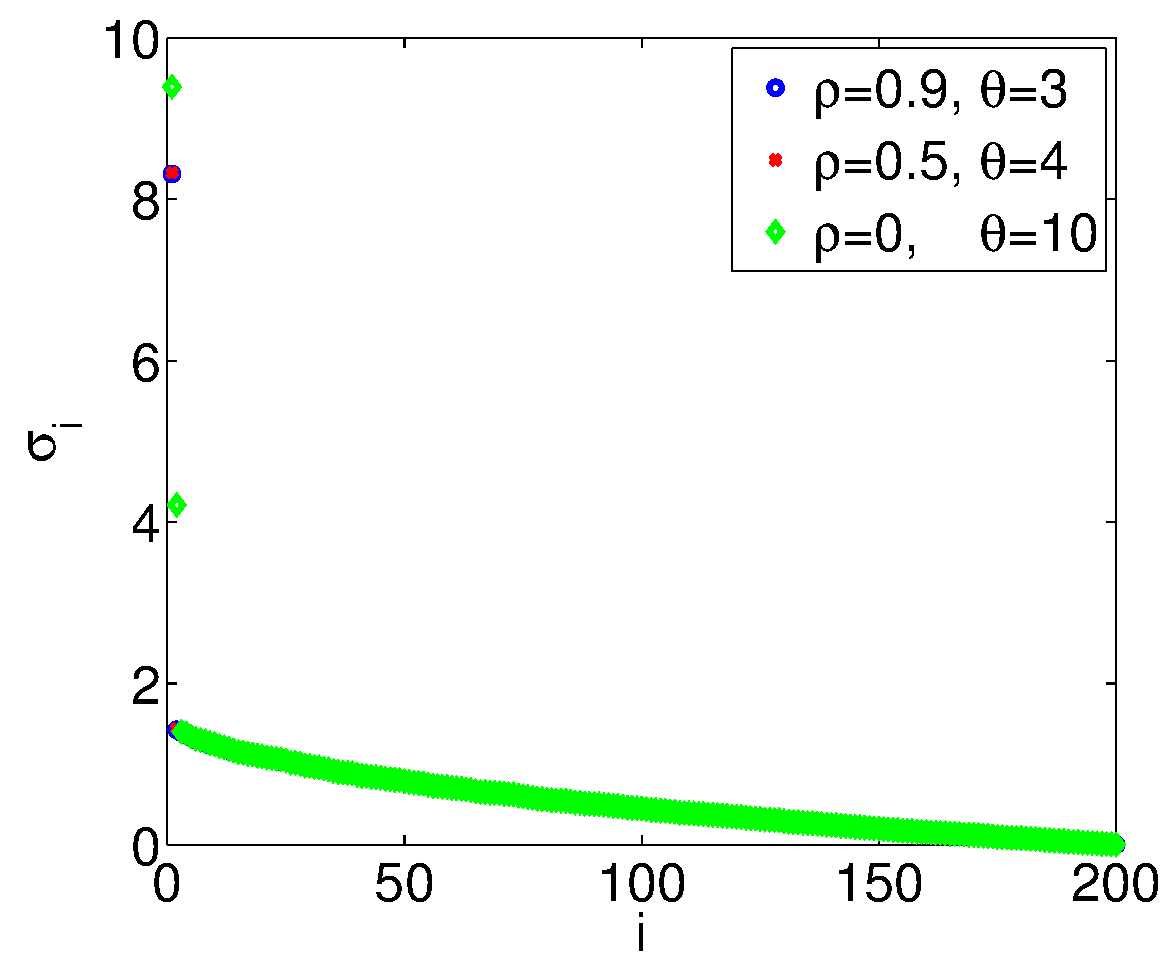
\includegraphics[width=0.4\textwidth]{figures/xy_motiv_all.pdf}
  \end{center}


\end{frame}

%%%%%%%%%%%%%%%%%%%%%%%%%%%%%%%%%%%%%%%%%%%%%
\begin{frame}{Singular Value Prediction of $XY^H$}

  \begin{Th}[Top singular values of LRCCA]
    Under low rank assumptions on $X$ and $Y$, the maximum singular values of
    $\frac{1}{n}XYHT$ solve
    \be\ba
    &0=\prod_{i=1}^r&&\left[\left(\varphi_H(\sigma_i)\varphi_F(\sigma_i) -
      \frac{1}{\theta_{yi}^2}\right)\left(\varphi_J(\sigma_i)\varphi_G(\sigma_i) -
      \frac{1}{\theta_{xi}^2}\right)\right. \\
      &&& \left.-\rho_i^2\varphi_H(\sigma_i)\varphi_G(\sigma_i)\left(1+\varphi_K(\sigma_i)\right)^2\right]\\
    \ea\ee
    where $\varphi(\cdot)$ are functions of the Stieltjes transforms of matrix products
    involving $R = X^HX$ and $S=Y^HY$.
  \end{Th}

\end{frame}


%%%%%%%%%%%%%%%%%%%%%%%%%%%%%%%%%%%%%%%%%%%%%
\begin{frame}{Singular Value Prediction of $XY^H$}

  \textbf{Simulation parameters}
  \begin{itemize}
  \item $p=200$, $q=400$, $n=400$
  \item $r=1$, $\rho = 1$
  \item $\theta=\theta_x=\theta_y$ 
  \item Numerically solve above equation using RMTool
  \end{itemize}

  \vspace{2ex}

  \begin{figure}
    \begin{center}
        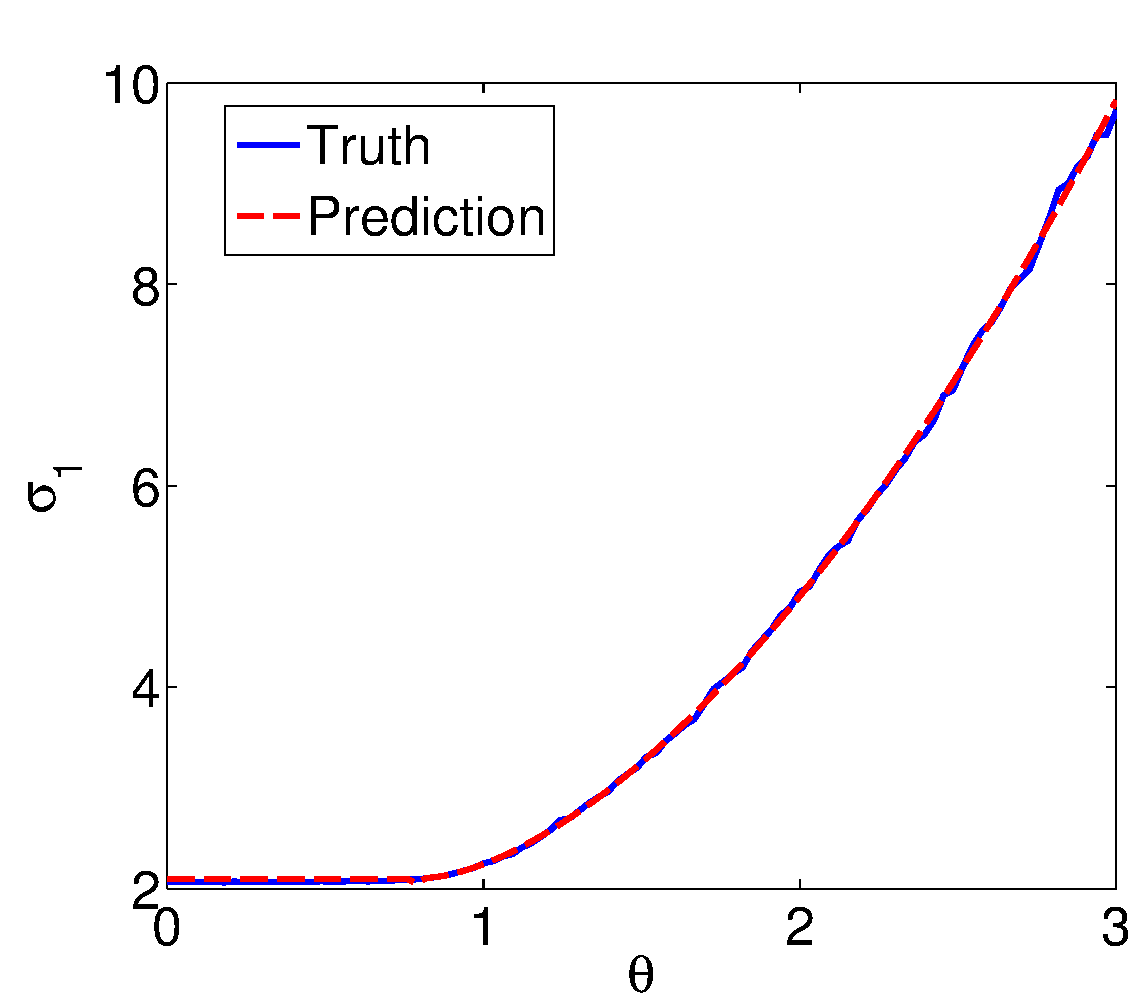
\includegraphics[width=0.5\textwidth]{figures/sigma_pred.pdf}
    \end{center}
  \end{figure}

\end{frame}

%%%%%%%%%%%%%%%%%%%%%%%%%%%%%%%%%%%%%%%%%%%%%
\begin{frame}{Phase Transition Prediction of $XY^H$}

  \fcolorbox{black}[HTML]{F1F1F1}{\parbox{1\textwidth}{
      \be
      0=\left(\varphi_H(b)\varphi_F(b) - \frac{1}{\theta_{y}^2}\right)\left(\varphi_J(b)\varphi_G(b) -
        \frac{1}{\theta_{x}^2}\right) - \rho^2\varphi_H(b)\varphi_G(b)\left(1+\varphi_K(b)\right)^2
      \ee
    }}

  \vspace{2ex}

  \textbf{Simulation parameters}
  \begin{itemize}
  \item $b= \sigma_1(XY^H)$ 
  \item $p=200$, $q=400$, $n=400$, $r=1$    
  \item Numerically solve above equation using RMTool
  \item Plot log of KS-statistic
  \end{itemize}

  \begin{center}
    $\boldsymbol{\rho=}\mathbf{0}$\hspace{18ex}$\boldsymbol{\rho=0.6}$\hspace{18ex}$\boldsymbol{\rho=1}$\\[0.5ex]
    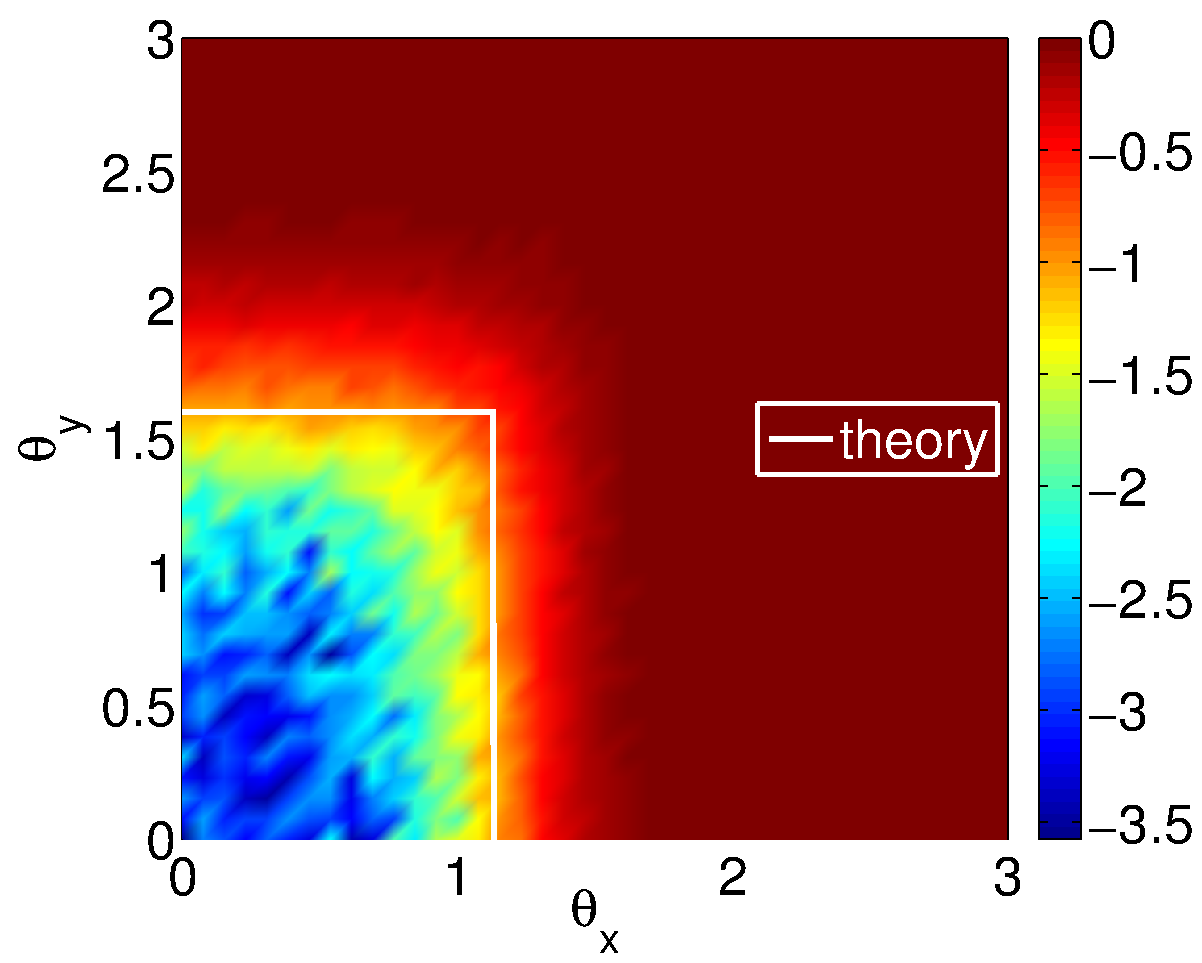
\includegraphics[width=0.3\textwidth]{figures/rho_0_theta.pdf}\hspace{1ex}
    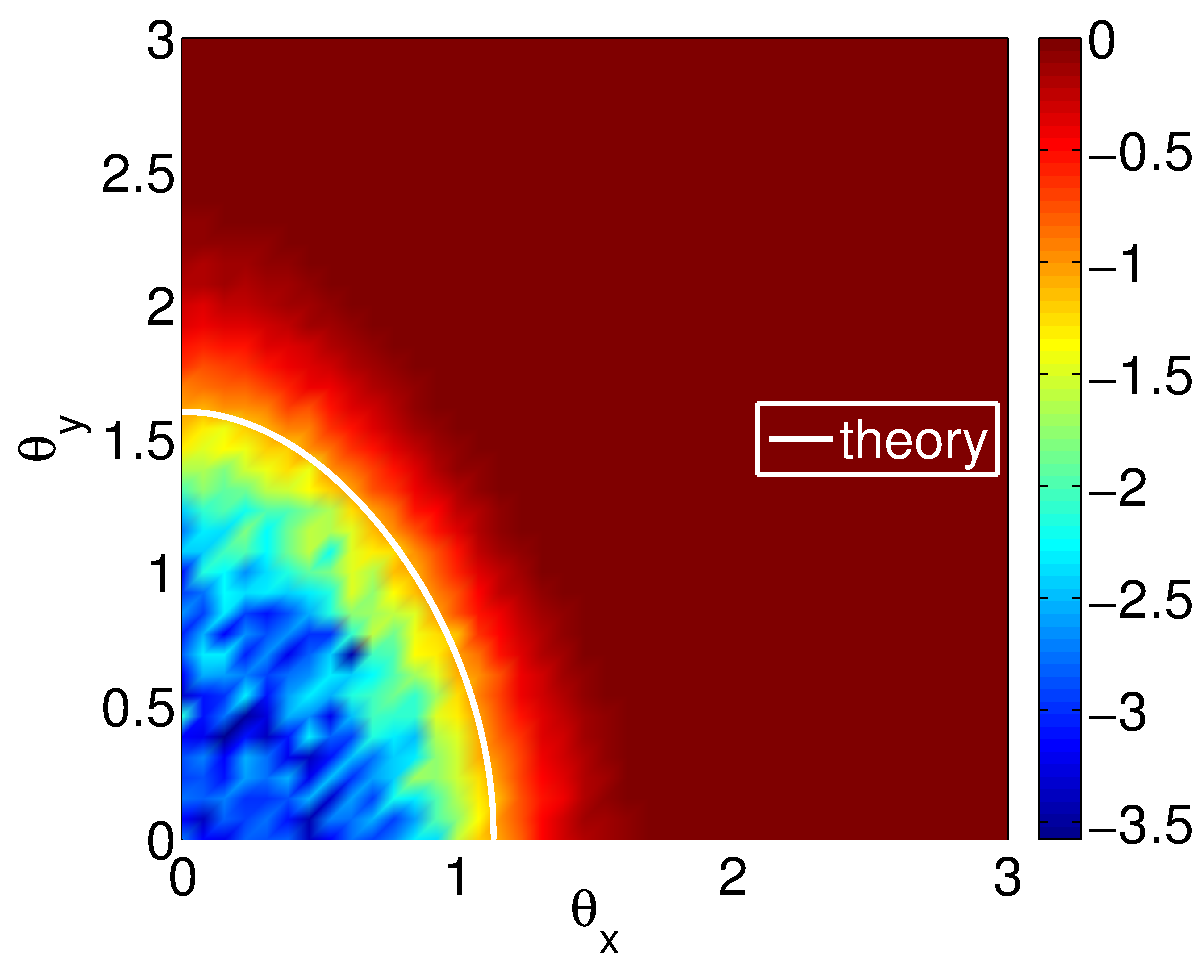
\includegraphics[width=0.3\textwidth]{figures/rho_6_theta.pdf}\hspace{1ex}
    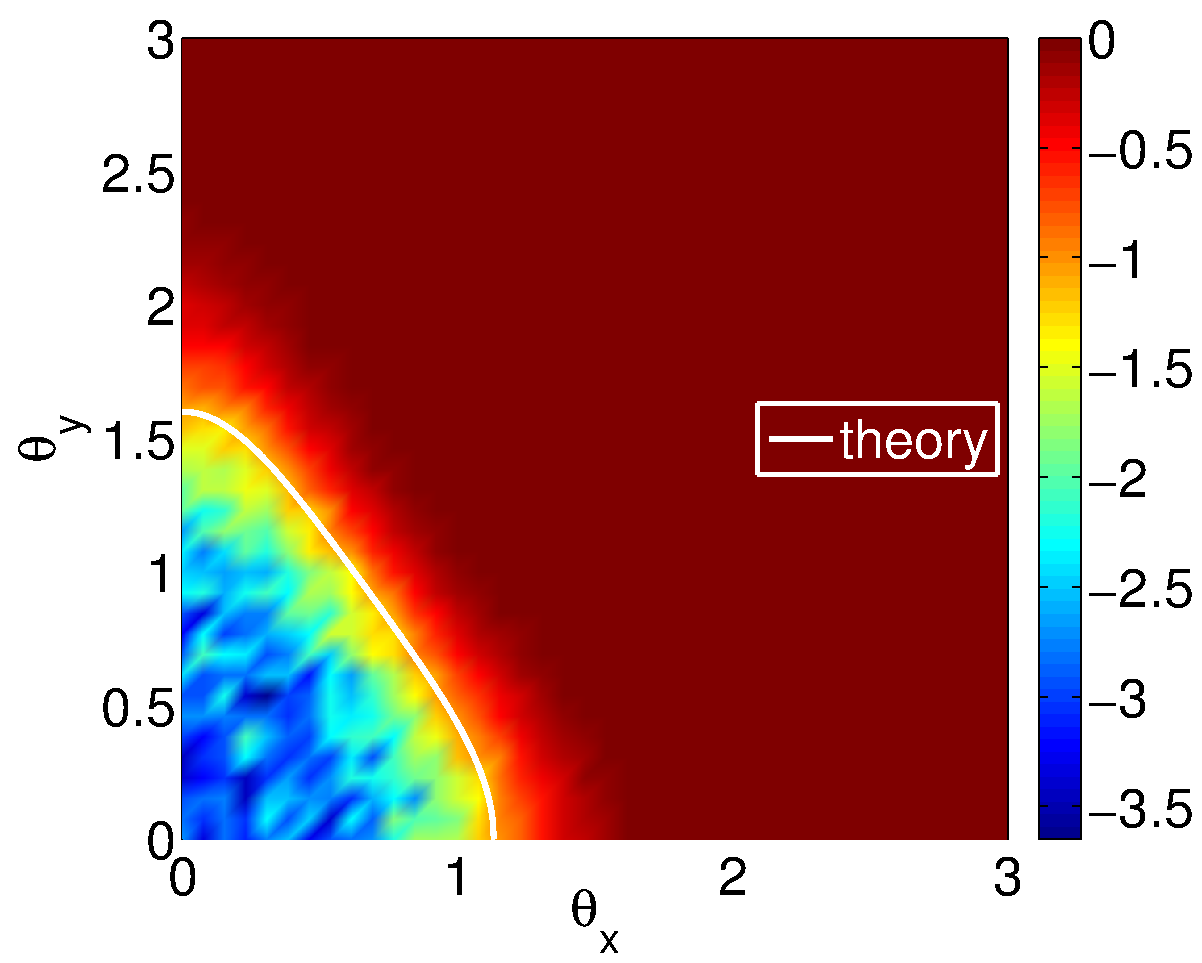
\includegraphics[width=0.3\textwidth]{figures/rho_10_theta.pdf}
  \end{center}

\end{frame}

\begin{frame}{Returning to Motivational Example}

  \textbf{What about using SNR estimates?}
  \begin{itemize}
  \item Estimate $\theta_x$ and $\theta_y$ from individual datasets
  \item Whiten the singular values of $\Rxyhat$ 
  \item This is CCA/ICCA!!
  \end{itemize}

  \vspace{2ex}

  \begin{center}
  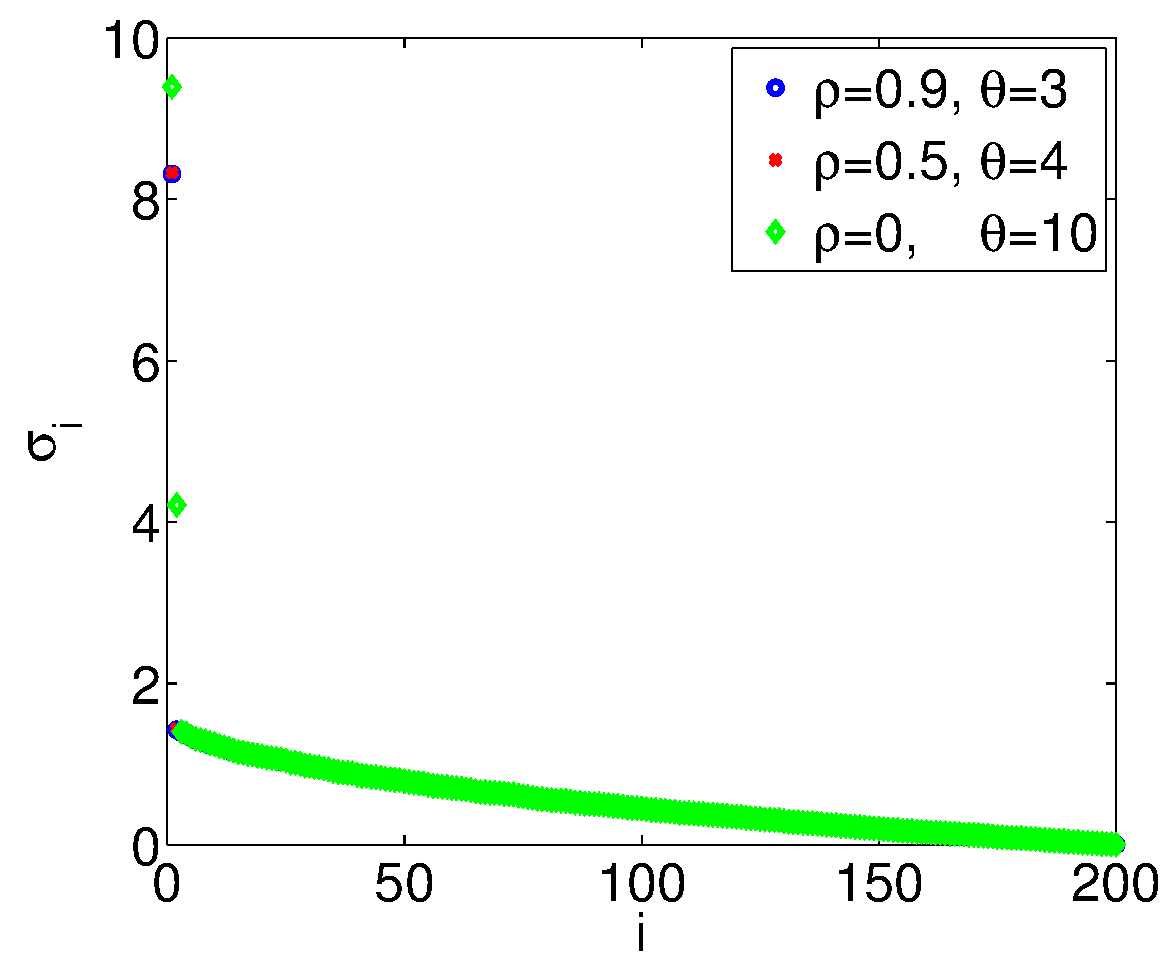
\includegraphics[width=0.5\textwidth]{figures/xy_motiv_all.pdf}
  \end{center}


\end{frame}

%%%%%%%%%%%%%%%%%%%%%%%%%%%%%%%%%%%%%%%%%%%%%
\begin{frame}{Signal Detection Using Random Projections}

  \begin{center}
    \textbf{Signal-plus-noise Matrix}\\
    \fcolorbox{black}[HTML]{F1F1F1}{\parbox{0.5\textwidth}{
        \be
        \widetilde{X}_n= \sum_{i=1}^r\theta_i u_iv_i^T + X_n.
        \ee    
      }}
  \end{center}

\vspace{3ex}

  \textbf{Parameters}
  \begin{itemize}
  \item $\theta_i>0$ for $i=1,\dots, r$
  \item $u_i^Hu_j=\delta_{\left\{i=j\right\}}$ and $v_i^Hv_j = \delta_{\left\{i=j\right\}}$.
  \item $u_i\in\complex^{n\times 1}$, $v_i\in\complex^{N\times 1}$
  \item $X_n$ is a random matrix with  $\mu_{X_n} =
    \frac{1}{\min(n,N)}\sum_{i=1}^{\min(n,N)}\delta_{\sigma_i}.$
  \item $\mu_{X_n}\to \mu_X$
  \end{itemize}

\end{frame}

\begin{frame}{Signal Detection Using Random Projections}

\textbf{Motivation}
\begin{itemize}
\item When $n$ is large, SVD of $\widetilde{X}_n$ is expensive
\item The detection limit of  $\widetilde{X}_n$ is $\theta> \left(\frac{n}{N}\right)^{1/4}$
\item Project to lower-dim space to save computation, $m < n$
\item This will result in a performance loss
\end{itemize}

\vspace{2ex}

\begin{columns}
  \begin{column}{0.4\textwidth}
  \begin{center}
  \textbf{Projections}\\
    \fcolorbox{black}[HTML]{F1F1F1}{\parbox{0.8\textwidth}{
        \be\ba
        &Y_n^G = G_n^H\widetilde{X}_n\\
        &Y_n^Q = Q_n^H\widetilde{X}_n\\
        \ea\ee
      }}
  \end{center}
  \end{column}
  \begin{column}{0.6\textwidth}
    \vspace{2ex}
    \begin{itemize}
    \item $G_n\in\complex^{n\times m}$ with independent $\mathcal{CN}(0,1)$ entries
    \item $Q_n\in\complex^{n\times m}$ s.t. $Q_n^HQ_n = I_m$
    \end{itemize}
  \end{column}
\end{columns}

\vspace{3ex}

\begin{center}
\textbf{Goal}\\
\fcolorbox{black}[HTML]{F1F1F1}{\parbox{0.6\textwidth}{
    \centering
    Quantify the performance loss as a function of $m,n,N,\theta$ when using the SVD of
    $Y_n^G$ and $Y_n^Q$ to detect signals 
  }}
\end{center}

\end{frame}

\begin{frame}{Main Result}
\begin{Th}[Largest singular values]
Let $Y_n$ be the projection of $\widetilde{X}_n$ onto either $G_n$ or $Q_n$. The largest
$r$ singular values of the $m\times N$ matrix $Y_n$ exhibit the 
following behavior as $n,m,N\to\infty$ with $n/N\to c_1$ and $m/N\to c_2$. We have that
for each fixed $1\leq i\leq r$, $\sigma_i\left(Y_n\right)$ solves
\beq\label{eq:chpt7:solution}
\sigma_i^2\varphi_F(\sigma_i)\varphi_H(\sigma_i) = \frac{1}{\theta_i^2},
\eeq
where
\be\ba
&\varphi_{F}(\sigma_i)\convas-\E{xm_{\mu_{RS|R}}\left(\sigma_i^2,x\right)}_{\mu_R}\\
&\varphi_{H}(\sigma_i)\convas-\frac{n}{N}m_{M_3}(\sigma_i^2) - \frac{1}{\sigma_i^2}\frac{n-N}{N}
\ea\ee
where $m_{\mu_M}$ is the Stieltjes transform of a matrix $M$
and $\mu_R$ is the limiting eigenvalue density of either $G_nG_n^H$ or $Q_nQ_n^H$,
$\mu_S$ is the limiting eigenvalue density of $X_nX_n^H$ and $M_3$
is either $G_nG_n^HX_nX_n^H$ or $Q_nQ_n^HX_nX_n^H$. 

\end{Th}
\end{frame}

\begin{frame}{Corollaries to Main Result}
\begin{Corr}[Phase transition]
When 
\be
\theta_i \leq \theta_{\text{crit}} = \frac{1}{b\sqrt{\varphi_F(b)\varphi_H(b)}}
\ee
Then 
\be
\sigma_i\convas b,
\ee
where $b$ is the supremum of the support of the limiting density of $G_n^HX_n$ or $Q_n^HX_n$.
\end{Corr}

\vspace{3ex}

\begin{Corr}[Unitary closed form]
When $Y_n$ is generated using a unitary matrix $Q_n$, 
\be
\sigma_i \convas \begin{cases} \sqrt{\frac{c_1}{\theta_i^2}+c_2\theta_i^2+1+c_1c_2} & \text{if }
  \theta_i\geq\left(\frac{c_1}{c_2}\right)^{1/4}\\ \sqrt{c_1c_2} +1 & \text{if }
    \theta_i<\left(\frac{c_1}{c_2}\right)^{1/4} \end{cases}
\ee
\end{Corr}

\end{frame}

\begin{frame}{Numerical Verification}

  \textbf{\hspace{27ex}$m=100$\hspace{17ex}$N=1000$}
  \begin{columns}
    \begin{column}{0.15\textwidth}
      \vspace{15ex}
      \textbf{Gaussian}\\
      \vspace{5ex}
      \textbf{Unitary}\\
    \end{column}
    \begin{column}{0.85\textwidth}
      \setcounter{subfigure}{0}
      \begin{figure}
        \begin{center}
          \subfigure{
            \label{fig:gauss1}
            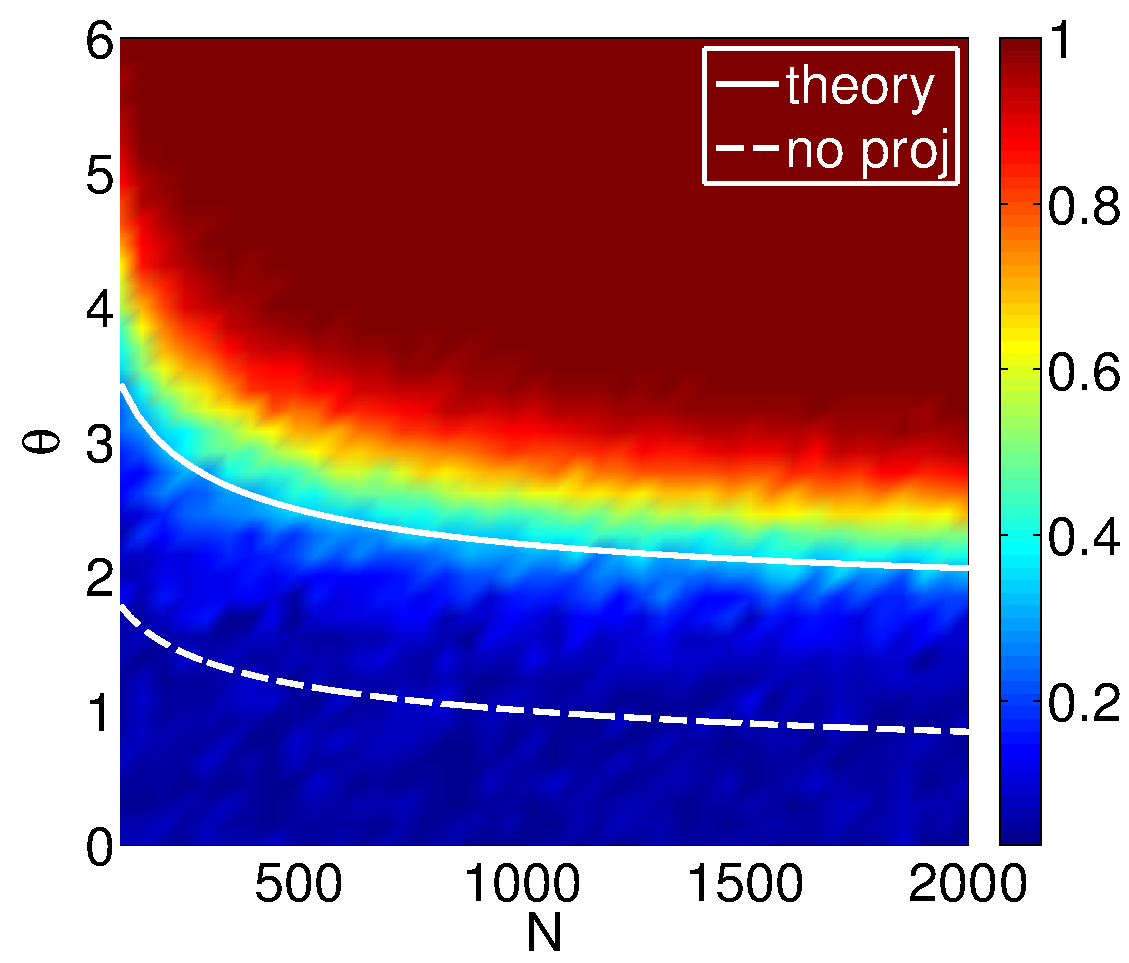
\includegraphics[width=0.4\textwidth]{figures/ks11.pdf}
          }
          \subfigure{
            \label{fig:gauss2}
            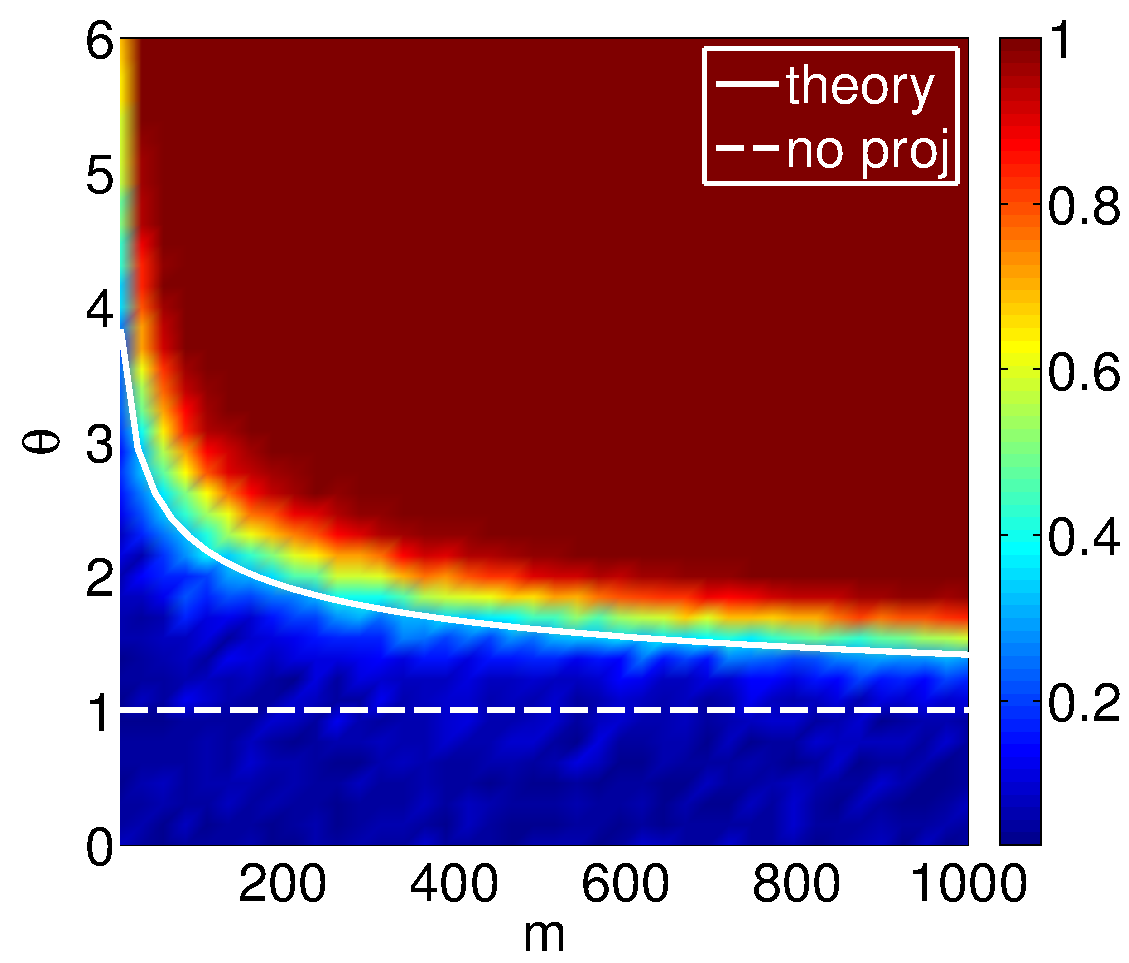
\includegraphics[width=0.4\textwidth]{figures/ks21.pdf}
          }
          \subfigure{
            \label{fig:ortho1}
            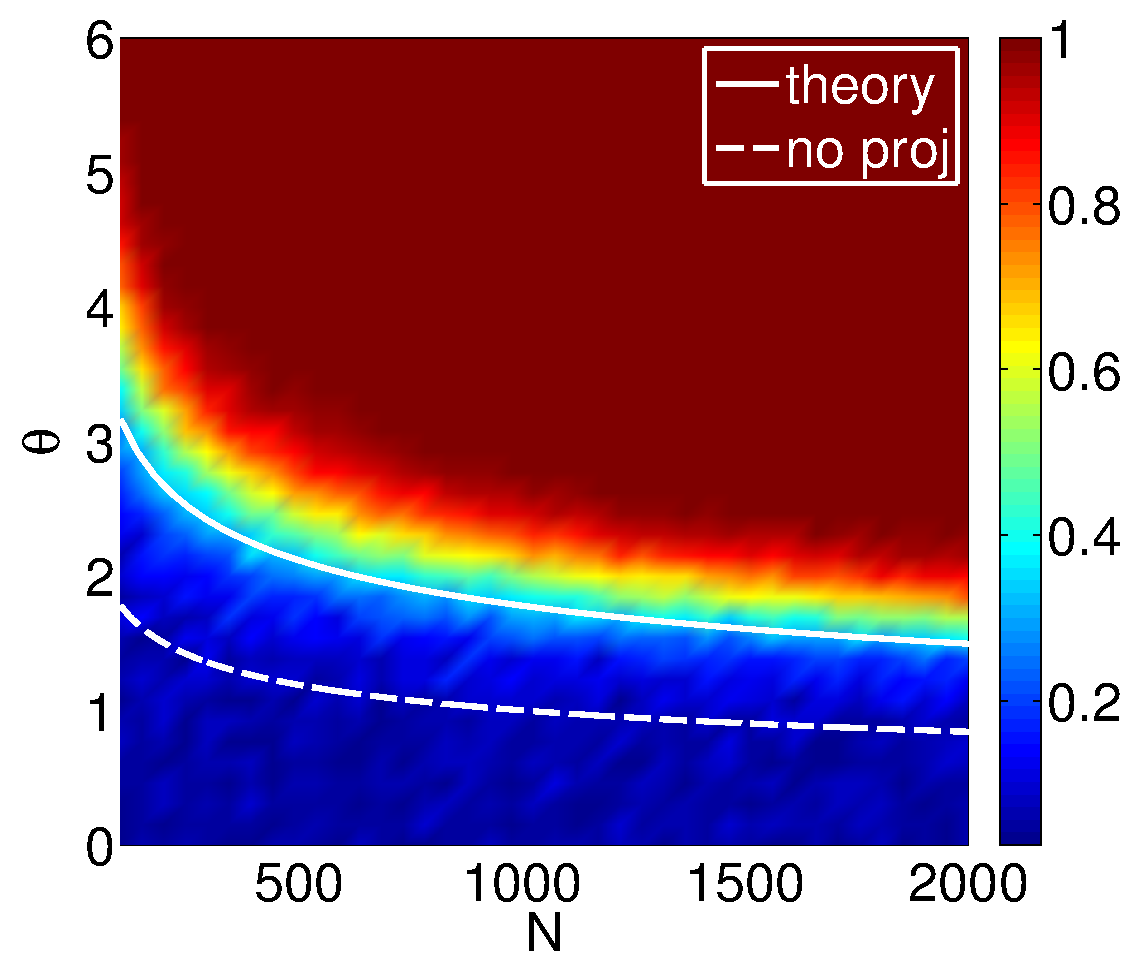
\includegraphics[width=0.4\textwidth]{figures/ks12.pdf}
          }
          \subfigure{
            \label{fig:ortho2}
            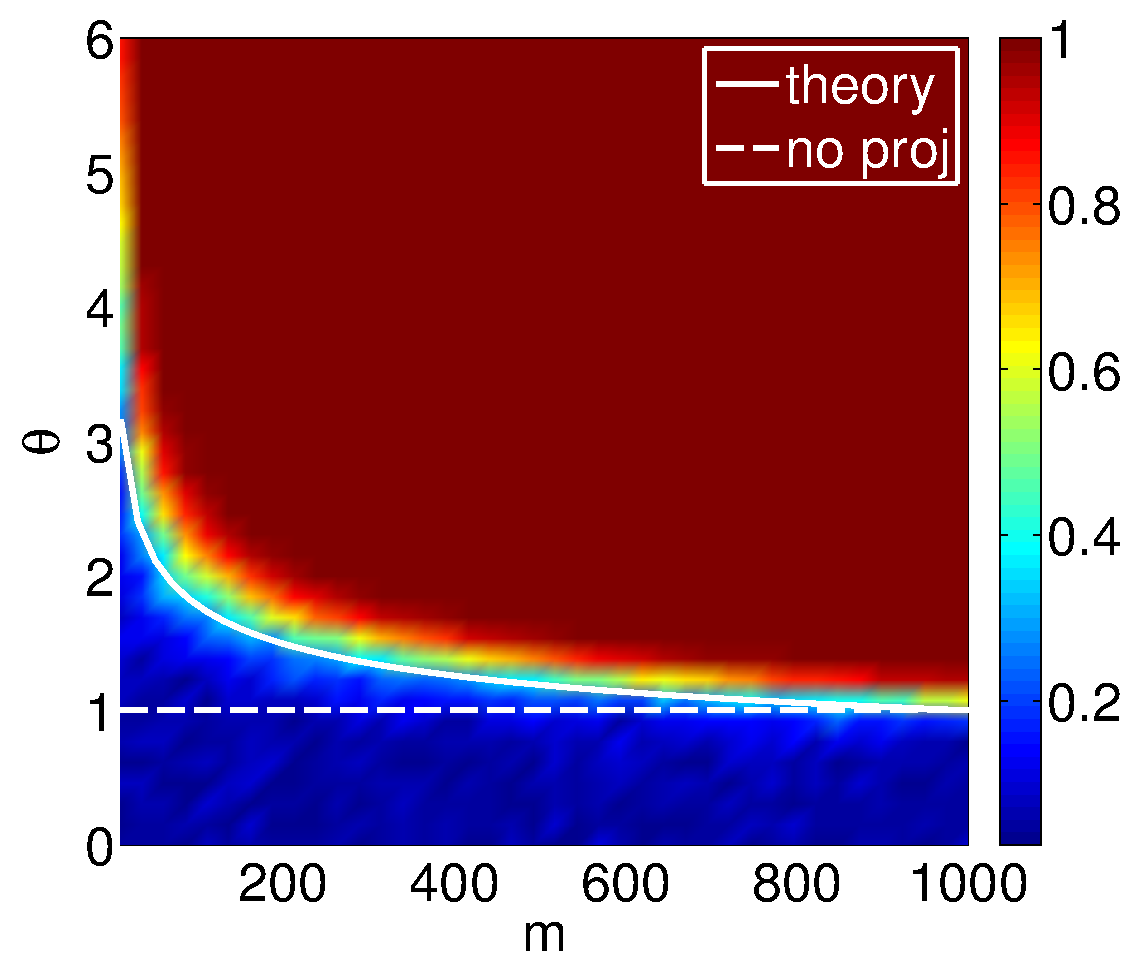
\includegraphics[width=0.4\textwidth]{figures/ks22.pdf}
          }
        \end{center}
      \end{figure}
    \end{column}
  \end{columns}
\end{frame}


\begin{frame}{Content Based Image Retrieval}

  \begin{columns}
    \begin{column}{0.5\textwidth}

      \centering
      \textbf{Training Data}

      \vspace{-3ex}

      \begin{figure}
        \begin{center}
          \begin{tikzpicture}[
            font=\sffamily,
            every matrix/.style={ampersand replacement=\&,column sep=4ex},
            dataset/.style={draw,thick,fill=yellow!20,inner sep=.3cm},
            ellip/.style={draw=none,inner sep=.3cm},
            sink/.style={dataset,rounded corners,fill=black, text=white},
            app/.style={dataset,rounded corners,fill=blue!20},
            dots/.style={gray,scale=2},
            to/.style={->,>=stealth,shorten >=2pt,thick,font=\sffamily\footnotesize},
            every node/.style={align=center}]

            \matrix{       
              \node (data1) {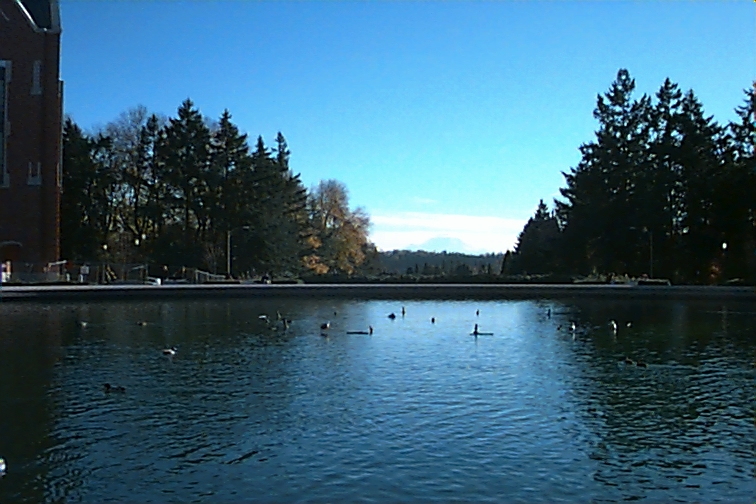
\includegraphics[width=0.5\textwidth]{figures/img_145.jpg}};
              \&\node[dataset] (cap1) {Caption 1};\\

              \node (data2) {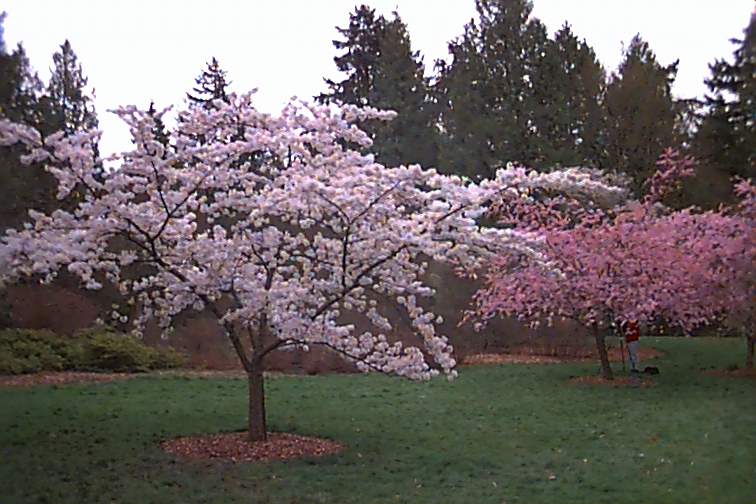
\includegraphics[width=0.5\textwidth]{figures/img_245.jpg}};
              \&\node[dataset] (cap2) {Caption 2};\\

              \node[ellip] (ell1) {$\vdots$};
              \&\node[ellip] (ell2) {$\vdots$};\\

              \node (data3) {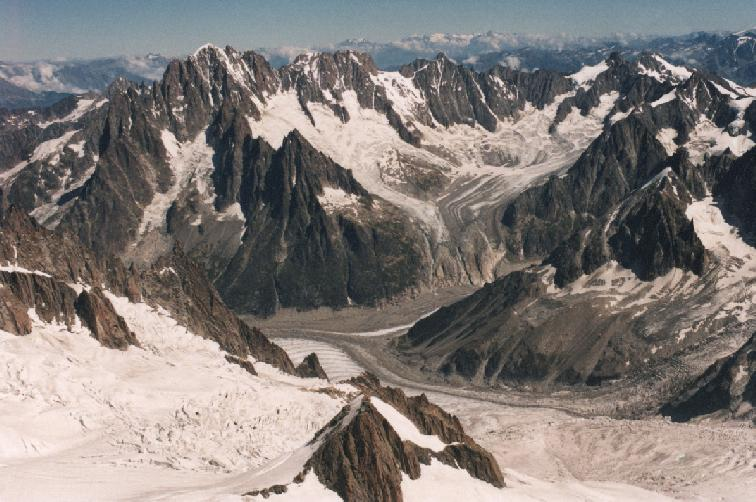
\includegraphics[width=0.5\textwidth]{figures/img_1049.jpg}};
              \&\node[dataset] (cap3) {Caption $n$};\\
            };

            \draw[to] (data1) -- (cap1) node[midway,left] {};
            \draw[to] (data2) -- (cap2) node[midway,left] {};
            \draw[to] (data3) -- (cap3) node[midway,left] {};

          \end{tikzpicture}
        \end{center}
      \end{figure}
    \end{column}
    \begin{column}{0.5\textwidth}
      \centering
      \textbf{Text Query}
      \begin{empheq}[box={\mybluebox[5pt][5pt][boxgrey]}]{equation*}
        \begin{aligned}
          & \text{snowy mountains}
        \end{aligned}
      \end{empheq}
      \Huge
      $$\Downarrow$$

      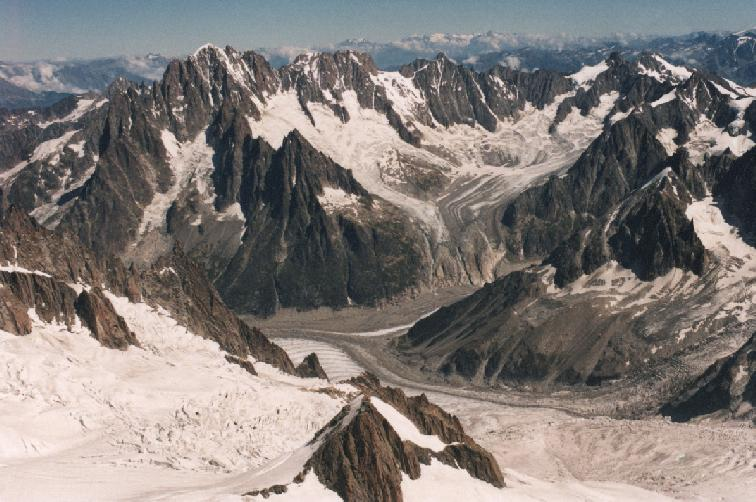
\includegraphics[width=0.5\textwidth]{figures/img_1049.jpg}
      

    \end{column}
  \end{columns}
\end{frame}

%%%%%%%%%%%%%%%%%
% Frame 2
%%%%%%%%%%%%%%%%%
\begin{frame}{Automatic Image Annotation}
  \begin{columns}
    \begin{column}{0.5\textwidth}

      \centering
      \textbf{Training Data}

      \vspace{-3ex}

      \begin{figure}
        \begin{center}
          \begin{tikzpicture}[
            font=\sffamily,
            every matrix/.style={ampersand replacement=\&,column sep=4ex},
            dataset/.style={draw,thick,fill=yellow!20,inner sep=.3cm},
            ellip/.style={draw=none,inner sep=.3cm},
            sink/.style={dataset,rounded corners,fill=black, text=white},
            app/.style={dataset,rounded corners,fill=blue!20},
            dots/.style={gray,scale=2},
            to/.style={->,>=stealth,shorten >=2pt,thick,font=\sffamily\footnotesize},
            every node/.style={align=center}]

            \matrix{       
              \node (data1) {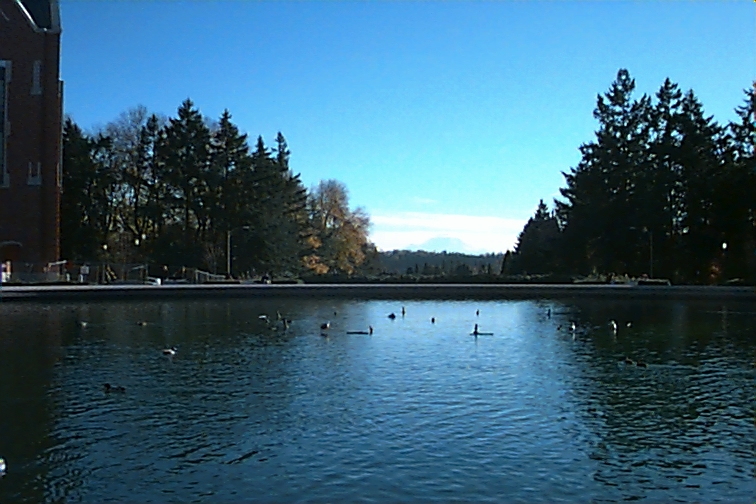
\includegraphics[width=0.5\textwidth]{figures/img_145.jpg}};
              \&\node[dataset] (cap1) {Caption 1};\\

              \node (data2) {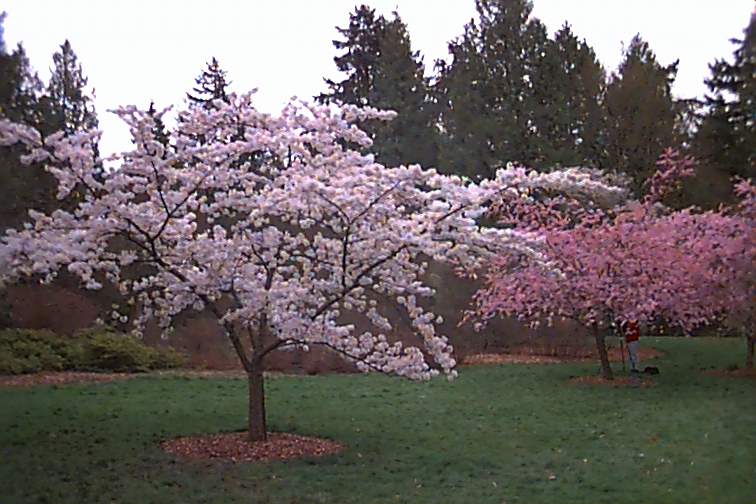
\includegraphics[width=0.5\textwidth]{figures/img_245.jpg}};
              \&\node[dataset] (cap2) {Caption 2};\\

              \node[ellip] (ell1) {$\vdots$};
              \&\node[ellip] (ell2) {$\vdots$};\\

              \node (data3) {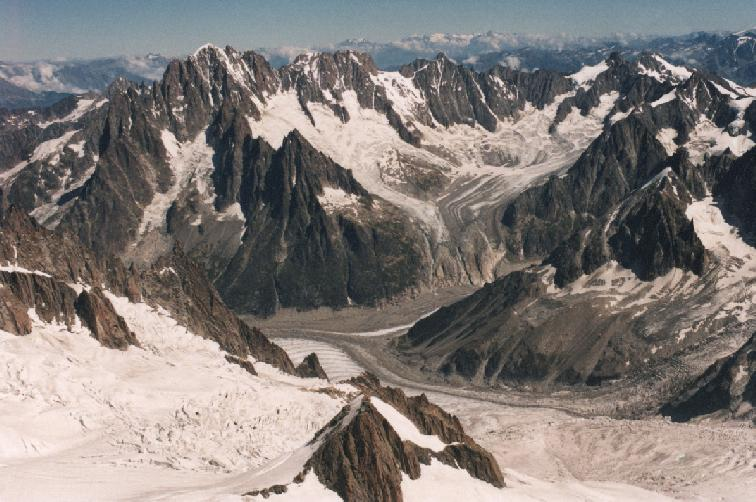
\includegraphics[width=0.5\textwidth]{figures/img_1049.jpg}};
              \&\node[dataset] (cap3) {Caption $n$};\\
            };

            \draw[to] (data1) -- (cap1) node[midway,left] {};
            \draw[to] (data2) -- (cap2) node[midway,left] {};
            \draw[to] (data3) -- (cap3) node[midway,left] {};

          \end{tikzpicture}
        \end{center}
      \end{figure}
    \end{column}
    \begin{column}{0.5\textwidth}
      \centering
      \textbf{Image Query}\\
      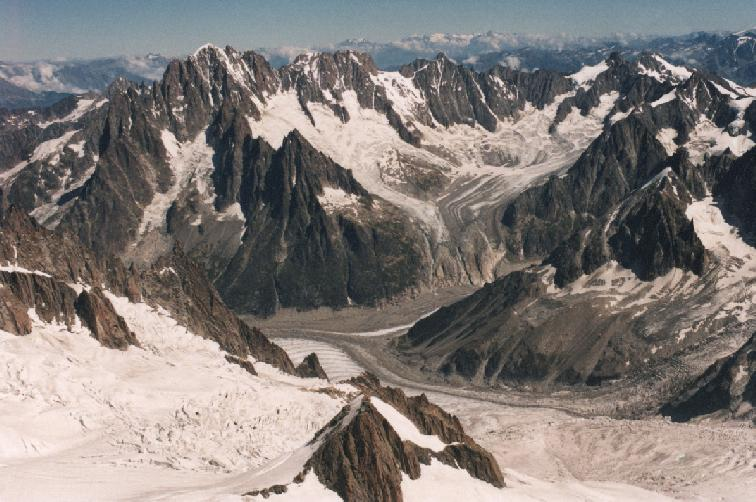
\includegraphics[width=0.5\textwidth]{figures/img_1049.jpg}
      {\Huge      $$\Downarrow$$}
      \begin{empheq}[box={\mybluebox[5pt][5pt][boxgrey]}]{equation*}
        \begin{aligned}
          & \text{snowy mountains}
        \end{aligned}
      \end{empheq}

    \end{column}
  \end{columns}
\end{frame}

\begin{frame}{Correlation Based Approaches}

  \textbf{Intuition}
  \begin{itemize}
  \item Image features are correlated to words
  \item CCA/ICCA seem like natural algorithms to identify correlations
  \end{itemize}

  \vspace{2ex}

  \textbf{Text Processing - \textit{\textcolor{textred}{tf}*\textcolor{texthigh}{idf}} feature vectors}
  \begin{itemize}
  \item \textcolor{textred}{term frequency} (\textit{tf}): frequent words are important
  \item \textcolor{texthigh}{inverse document frequency} (\textit{idf}): unique document words are important
  \item optional Porter stemming and stopword removal
  \end{itemize}

  \vspace{2ex}

  \textbf{Image Processing - Visual Words}
  \begin{enumerate}
  \item create SIFT features for all training images
  \item k-mean clustering of all SIFT features to ``visual words''
  \item assign each SIFT keypoint to closest visual word
  \item bag of words count the occurrences of visual word in each image
  \end{enumerate}

\end{frame}

\begin{frame}{Training Pipeline}

\begin{figure}
  \begin{center}
    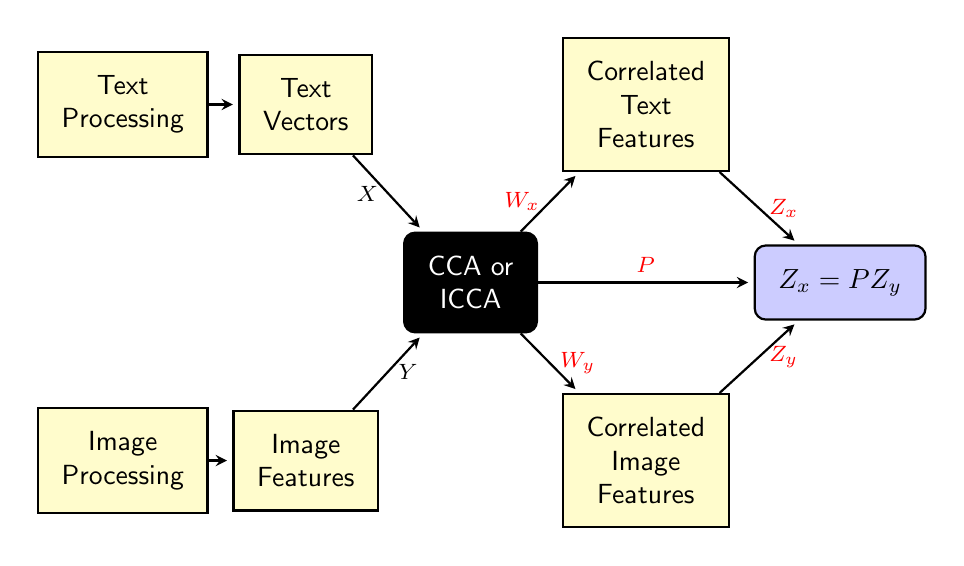
\begin{tikzpicture}[
      font=\sffamily,
      every matrix/.style={ampersand replacement=\&,column sep=2ex,row sep=5ex},
      dataset/.style={draw,thick,fill=yellow!20,inner sep=.3cm},
      sink/.style={dataset,rounded corners,fill=black, text=white},
      app/.style={dataset,rounded corners,fill=blue!20},
      dots/.style={gray,scale=2},
      to/.style={->,>=stealth,shorten >=2pt,thick,font=\sffamily\footnotesize},
      every node/.style={align=center}]

      \matrix{       
        \node[dataset] (textp) {Text \\ Processing};
        \& \node[dataset] (dataset1) {Text \\Vectors};
        \& ;
        \& \node[dataset] (dataset3) {Correlated \\Text \\Features};
        \&; \\

        ; 
        \& ;
        \& \node[sink] (blackbox) {CCA or\\ ICCA}; 
        \& ;
        \& \node[app] (application) {$Z_x=PZ_y$};\\

        \node[dataset] (imp) {Image \\Processing};
        \& \node[dataset] (dataset2) {Image \\Features};
        \& ;
        \& \node[dataset] (dataset4) {Correlated\\ Image\\ Features};
        \& ;\\
      };

      \draw[to] (textp) -- (dataset1)node[midway,left] {};
      \draw[to] (imp) -- (dataset2)node[midway,right] {};
      \draw[to] (dataset1) -- (blackbox)node[midway,left] {$X$};
      \draw[to] (dataset2) -- (blackbox)node[midway,right] {$Y$};
      \draw[to] (blackbox) -- (dataset3) node[midway,left] {\textcolor{red}{$W_x$}};
      \draw[to] (blackbox) -- (dataset4) node[midway,right] {\textcolor{red}{$W_y$}};
      \draw[to] (blackbox) -- (application) node[midway,above] {\textcolor{red}{$P$}};
      \draw[to] (dataset3) -- (application) node[midway,right] {\textcolor{red}{$Z_x$}};
      \draw[to] (dataset4) -- (application) node[midway,right] {\textcolor{red}{$Z_y$}};
    \end{tikzpicture}
  \end{center}
\end{figure}

\end{frame}

\begin{frame}{Automatic Caption Annotation Pipeline}

\begin{figure}
  \begin{center}
    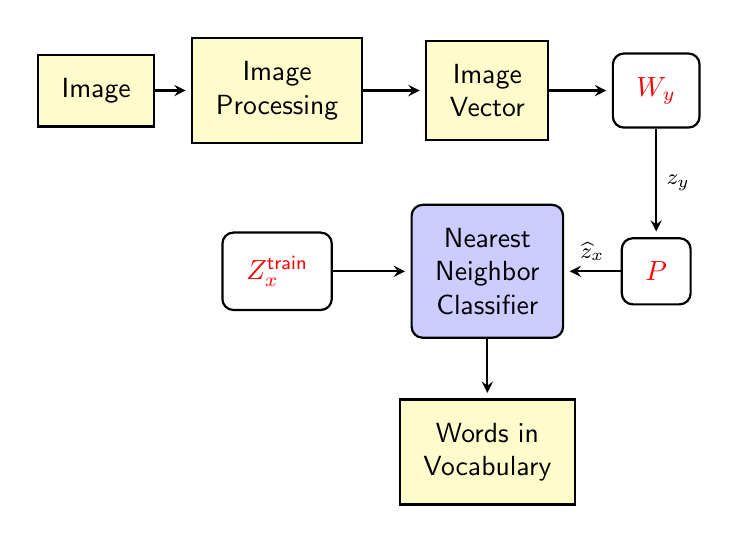
\begin{tikzpicture}[
      font=\sffamily,
      every matrix/.style={ampersand replacement=\&,column sep=3ex,row sep=5ex},
      dataset/.style={draw,thick,fill=yellow!20,inner sep=.3cm},
      sink/.style={dataset,rounded corners,fill=white, text=red},
      app/.style={dataset,rounded corners,fill=blue!20},
      dots/.style={gray,scale=2},
      to/.style={->,>=stealth,shorten >=2pt,thick,font=\sffamily\footnotesize},
      every node/.style={align=center}]


      \matrix{
        \node[dataset] (query) {Image};
        \& \node[dataset] (tp) {Image\\Processing};
        \& \node[dataset] (qv) {Image\\Vector};
        \&;\node[sink] (wx) {$W_y$};  \\

        ; 
        \& \node[sink] (zy) {$Z_x^{\text{train}}$}; 
        \& \node[app] (nn) {Nearest\\Neighbor\\Classifier};
        \& \node[sink] (P) {$P$}; \\

        ; 
        \& ;
        \& \node[dataset] (image) {Words in\\Vocabulary};
        \& \\
      };

      \draw[to] (query) -- (tp)node[midway,left] {};
      \draw[to] (tp) -- (qv)node[midway,right] {};
      \draw[to] (qv) -- (wx) node[midway,left] {};
      \draw[to] (wx) -- (P) node[midway,right] {$z_y$};
      \draw[to] (P) -- (nn) node[midway,above] {$\widehat{z}_x$};
      \draw[to] (zy) -- (nn) node[midway,right] {};
      \draw[to] (nn) -- (image) node[midway,right] {};


    \end{tikzpicture}
  \label{fig:training}
  \end{center}
\end{figure}

\end{frame}

\begin{frame}{Pascal Dataset}

  \textbf{Pascal Dataset}
  \begin{itemize}
  \item 1000 images each with 5 captions
  \item Vocabulary: 2393 words    
  \end{itemize}

\vspace{4ex}

\begin{figure}[T]
  \begin{minipage}{0.45\linewidth}
    \centering
    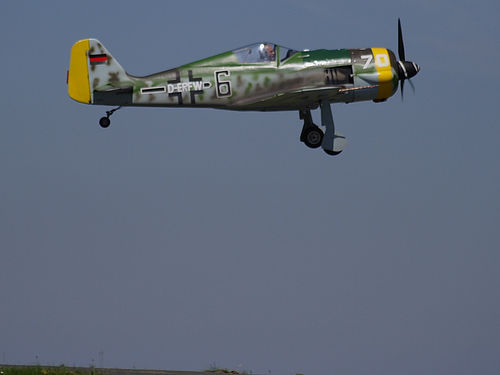
\includegraphics[width=.8\textwidth]{figures/img_3.jpg}
  \end{minipage}
  \begin{minipage}[t]{0.45\linewidth}
    \vspace{-10ex}
    \centering
    \footnotesize
    \begin{itemize}
    \item A D-ERFW-6 in flight.
    \item An army green plane flying in the sky.
    \item An old fighter plane flying with German military markings.
    \item A small green and yellow plane in the sky.
    \item A WWII fighter plane with its landing gear down.
    \end{itemize}
  \end{minipage}
\end{figure}



\end{frame}

%%%%%%%%%%%%%%%%%%%%%%%%%%%%%%%%%%%%%%%%%%%%%%%%%%%%%%%%%%%%%%%%%%%
\begin{frame}{Pascal Dataset - Image Retrieval}

\textbf{Text Query: } airplane

  \setcounter{subfigure}{0}
\begin{figure}[t]
  \centering
  \subfigure[CCA Results]{
    \centering
    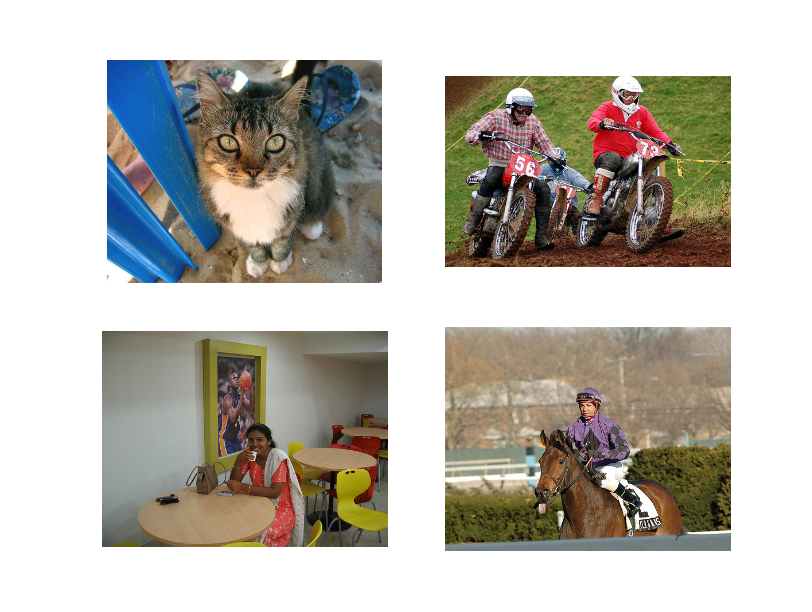
\includegraphics[width=0.45\textwidth]{figures/pascal_cca_ex.png}
    \label{fig:chpt9:CCA_query_results}}
  \subfigure[ICCA Results]{
    \centering
    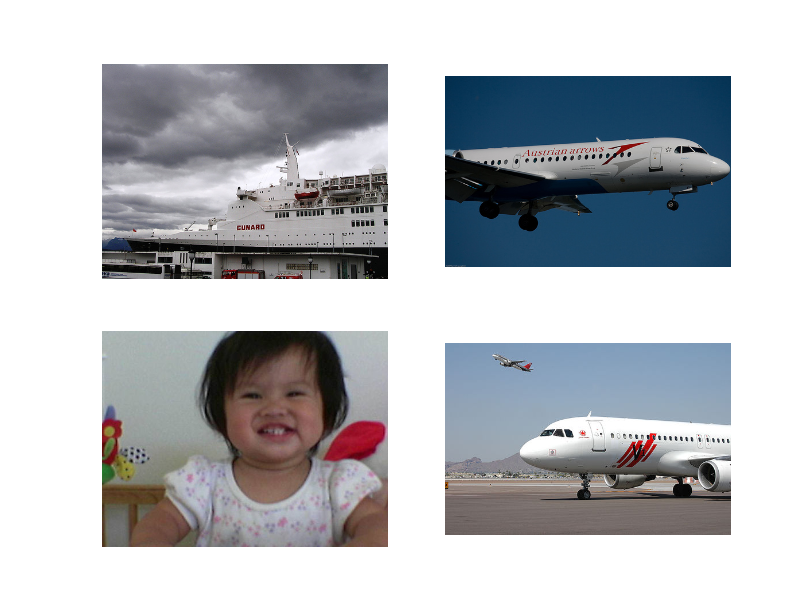
\includegraphics[width=0.45\textwidth]{figures/pascal_icca_ex.png}
    \label{fig:chpt9:ICCA_query_results}}
\end{figure}


\end{frame}


\begin{frame}{Pascal Dataset: Image Annotation}

\begin{columns}[T]
  \begin{column}{0.5\textwidth}
	\centering
    \textbf{Image Query}\\
	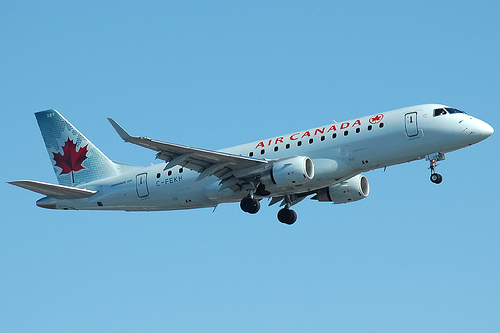
\includegraphics[width=0.8\textwidth]{figures/img_27.jpg}
  \end{column}
  \begin{column}{0.5\textwidth}
    \begin{minipage}[t]{0.4\textwidth}
      \small
      \begin{center}
        \textbf{CCA Annotation}
      \end{center}
      \begin{enumerate}
      \item hairless
      \item buddi
      \item swan
      \item leaf-less
      \item bnsf
      \item desert
      \item fluffi
      \item salad
      \item majest
      \item memorabilia
      \end{enumerate}
    \end{minipage}%
    \begin{minipage}[t]{0.1\textwidth}
    \end{minipage}
    \begin{minipage}[t]{0.4\textwidth}
      \small
      \begin{center}
        \textbf{ICCA Annotation}
      \end{center}
      \begin{enumerate}
      \item plane
      \item ship
      \item cruis
      \item fly
      \item blue
      \item jet
      \item airplan
      \item dock
      \item fighter
      \item through
      \end{enumerate}
    \end{minipage}
  \end{column}
\end{columns}
\end{frame}

%%%%%%%%%%%%%%%%%%%%%%%%%%%%%%%%%%%%%%%%%%%%
\begin{frame}{Application to Image Annotation}
 \textbf{University of Washington Ground Truth Dataset}
  \begin{itemize}
  \item 1109 image-label pairs
  \item Vocabulary 346 unique words
  \end{itemize}

  \vspace{2ex}

  \begin{columns}[T]

    \begin{column}{0.32\textwidth}
      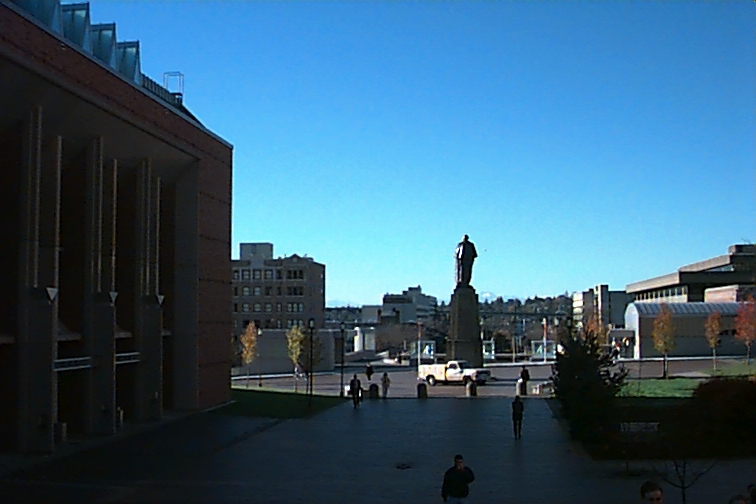
\includegraphics[width=1.1\textwidth]{figures/img_137.jpg}
      \vspace{2ex}
      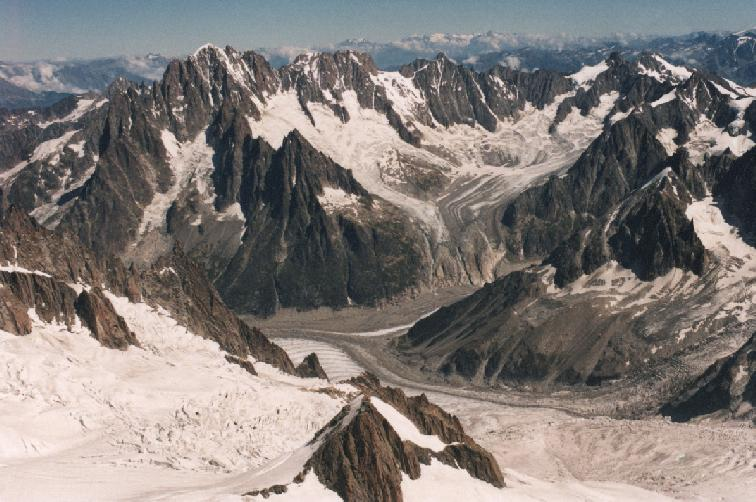
\includegraphics[width=1.1\textwidth]{figures/img_1049.jpg}      
    \end{column}%

    \begin{column}{0.3\textwidth}%
      \begin{center}
        \begin{empheq}[box={\mybluebox[5pt][5pt][boxgrey]}]{equation*}
          \begin{aligned}
            &\text{clear, sky, building,}\\
            &\text{ground, statue, people,}\\
            &\text{bush, grass, truck}\\
          \end{aligned}
        \end{empheq}
      \end{center}

      \vspace{1ex}

     \begin{center}
        \begin{empheq}[box={\mybluebox[5pt][5pt][boxgrey]}]{equation*}
          \begin{aligned}
            &\text{Clear, sky, snow,}\\
            &\text{Mountains, Rockes}\\
          \end{aligned}
        \end{empheq}
      \end{center}
    \end{column}

  \end{columns}
\end{frame}

%%%%%%%%%%%%%%%%%%%%%%%%%%%%%%%%%%%%%%%%%%%%%
\begin{frame}{Application to Image Annotation}

  \vspace{2ex}

  \begin{columns}[T]
   \begin{column}{0.5\textwidth}
      \centering
      \textbf{CCA}\\
      Mean Accuracy: 0.0184\\
      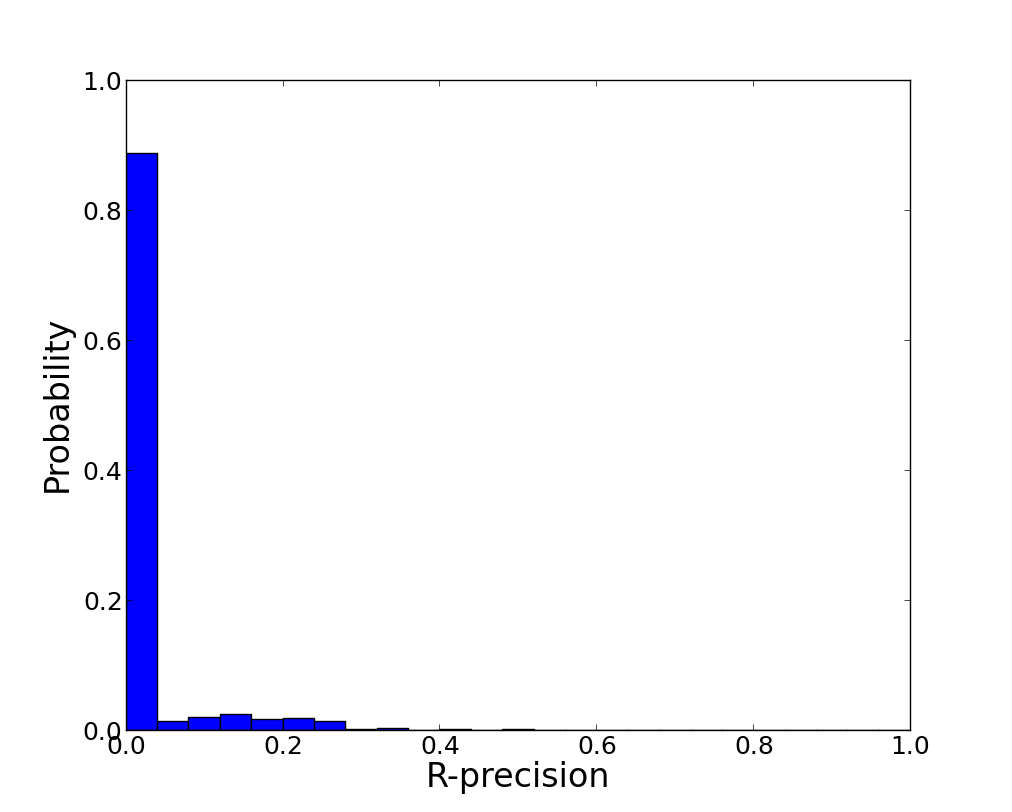
\includegraphics[width=1\textwidth]{figures/cca_rprec.png}
    \end{column}
    \begin{column}{0.5\textwidth}
      \centering
      \textbf{ICCA}\\
      Mean Accuracy: 0.2067\\
      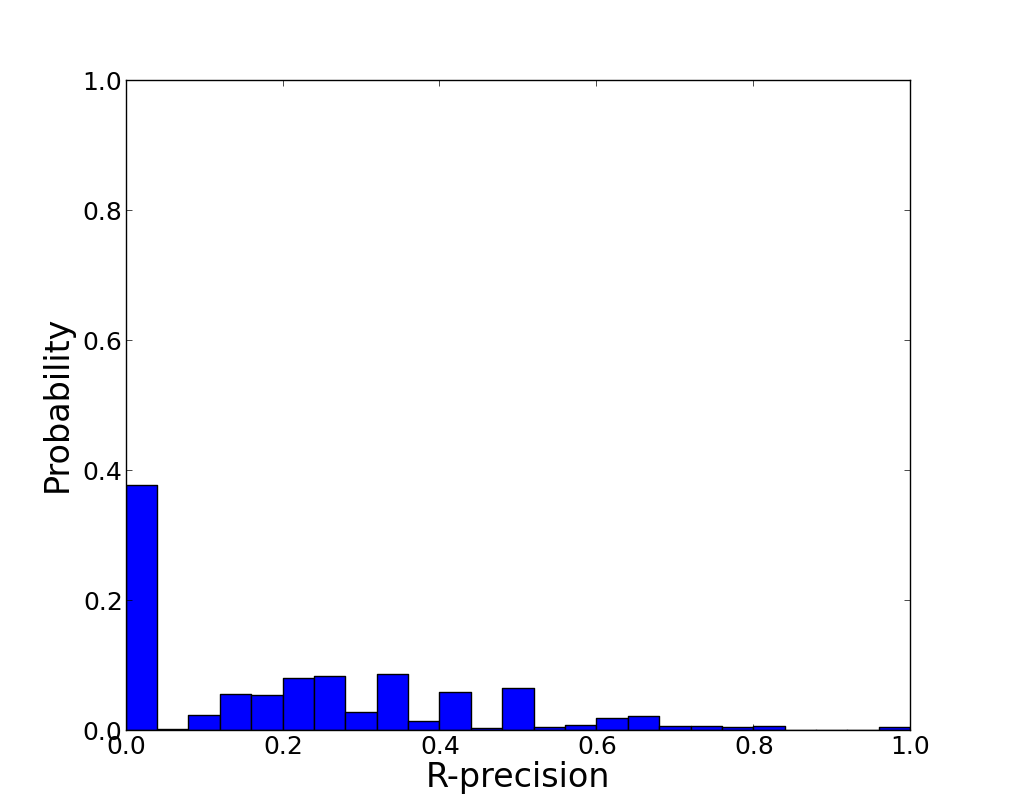
\includegraphics[width=1\textwidth]{figures/icca_rprec.png}
    \end{column}
  \end{columns}

\end{frame}


%%%%%%%%%%%%%%%%%%%%%%%%%%%%%%%%%%%%%%%%%%%%%%%%%%%%%%%%%%%%%%%%%%%%%%%
\begin{frame}{MCCA - Multiset CCA}

  \begin{center}
    \fcolorbox{black}[HTML]{F1F1F1}{\parbox{0.7\textwidth}{%
        \centering What if we have $m$ datasets $Y_1,\dots,Y_m$?  }}
  \end{center}

\vspace{1ex}

\textbf{Notation}
\begin{itemize}
\item covariance matrices: $R_{ij} = \E{y_iy_j^H}$
\item canonical vectors: $x_1,\dots,x_m$
\item canonical variates: $w_1,\dots, w_m$, $w_i=x_i^Hy_i$
\end{itemize}

\vspace{2ex}

\begin{equation*}
\Phi(x)=E[ww^H]=\left[\begin{array}{ccc} x_1^HR_{11}x_1 & \dots & x_1^HR_{1m}x_m \\ \vdots
    & \ddots & \vdots \\ x_m^HR_{m1}x_1 & \dots & x_m^HR_{mm}x_m\\ \end{array}\right]
\end{equation*}

\vspace{1ex}

\begin{center}
  \textbf{Optimization Problem}\\

  \fcolorbox{black}[HTML]{F1F1F1}{\parbox{0.5\textwidth}{%
      \be\ba
      &\underset{x}{\mathop{\rm optimize}} && J(\Phi(x))\\
      &\mathop{\rm subject to} && h(x,R)\\
      \ea\ee
    }}
\end{center}


\end{frame}

%%%%%%%%%%%%%%%%%%%%%%%%%%%%%%%%%%%%%%%%%%%%%%%%%%%%%%%%
\begin{frame}{MCCA - Multiset CCA}

  \begin{columns}[t]
    \begin{column}{0.5\textwidth}
      \centering\underline{\textbf{Ambiguity in Objective Function}}
      \begin{equation*}
        \begin{aligned}
          &\text{SUMCORR} &&\argmax_{x_1,\dots,x_m}\sum_{i=1}^m\sum_{j=1}^mx_i^HR_{ij}x_j\\[1ex]
          &\text{SSQCORR} &&\argmax_{x_1,\dots,x_m}\sum_{i=1}^m\sum_{j=1}^m\left(x_i^HR_{ij}x_j\right)^2\\[1ex]
          &\textcolor{textred}{\text{MAXVAR}} &&\textcolor{textred}{\argmax_{x_1,\dots,x_m}\lambda_1\left(\Phi(x)\right)}\\[1ex]
          &\textcolor{texthigh}{\text{MINVAR}} &&\textcolor{texthigh}{\argmin_{x_1,\dots,x_m}\lambda_m\left(\Phi(x)\right)}\\[1ex]
          &\text{GENVAR} &&\argmin_{x_1,\dots,x_m}\prod_{i=1}^m\lambda_i\left(\Phi(x)\right)\\[1ex]
        \end{aligned}
      \end{equation*}

    \end{column}
    \begin{column}{0.5\textwidth}
      \centering\underline{\textbf{Ambiguity in Constraint Function}}
      \begin{equation*}
        \begin{aligned}
          &\text{NORM} && \|x_i\|_2^2 =1\\[1ex]
          &\text{AVGNORM} &&\sum_{i=1}^m\|x_i\|_2^2 = m\\[1ex]
          &\textcolor{textred}{\text{VAR}} &&\textcolor{textred}{x_i^HR_{ii}x_i = 1}\\[1ex]
          &\text{AVGVAR} &&\sum_{i=1}^mx_i^HR_{ii}x_i = m\\[1ex]
        \end{aligned}
      \end{equation*}

    \end{column}
  \end{columns}

\end{frame}

%%%%%%%%%%%%%%%%%%%%%%%%%%%%%%%%%%%%%%%%%%%%%
\begin{frame}{MCCA - MAXVAR, VAR}

  \begin{center}
    \textbf{Objective Function}\\
    \fcolorbox{black}[HTML]{F1F1F1}{\parbox{0.4\textwidth}{%
        \be\ba
        &\argmax_{x_1,\dots,x_m}&&\lambda_1\left(\Phi(x)\right)\\
        &\text{subject to} &&x_i^HR_{ii}x_i = 1, \forall i
        \ea\ee
      }}
    \end{center}

  \begin{itemize}
  \item Let $V_i$ be the right singular vectors of dataset $Y_i$
  \end{itemize}

  \be
  \Cmcca=\left[\begin{array}{cccc} I_{d_1} & V_1^HV_2 & \cdots & V_1^HV_m\\
      V_2^HV_1 & I_{d_2} & \cdots & V_2^HV_m\\
      \vdots & \vdots & \ddots & \vdots\\
      V_m^HV_1 & V_m^HV_2 & \cdots & I_{d_m}\end{array}\right]
  \ee


  \begin{itemize}
  \item Let $\Cmcca = FKF^H$ be eigenvalue decomposition
  \item $\rho^{(j)} = k_j$
  \item $x_i = R_{ii}^{-1/2}f_i$
  \end{itemize}

\end{frame}

\begin{frame}{MAXVAR for CCA}

\textbf{Two dataset setting}
\be\ba
&C_{\text{cca}} && = \left[\begin{array}{c}V_1^H\\V_2^H\end{array}\right]\left[\begin{array}{cc}V_1 &
    V_2\end{array}\right] \\
&&&= \left[\begin{array}{cc}I_{d_1} &
    V_1^HV_2\\ V_2^HV_1 & I_{d_2}\end{array}\right]\\
&&&= \left[\begin{array}{cc}F & -F\\ G & G\end{array}\right]
\left[\begin{array}{cc}I + \left(KK^H\right)^{-1/2} & 0\\ 0 & I - \left(K^HK\right)^{-1/2}\end{array}\right]
\left[\begin{array}{cc}F & -F\\ G & G\end{array}\right]^H
\ea\ee

\vspace{2ex}

\textbf{Insights}
\begin{itemize}
\item Eigenvalues come in pairs $\left\{1+k_i,1-k_i,\right\}$
\item Perfect correlation implies $\lambda_{\text{max}}=2$, $\lambda_{\text{min}} = 0$
\item Eigenvectors have specific structure
\item MINVAR solves the same problem!
\item Correlation implies \textit{ALL} datasets correlated!
\end{itemize}


\end{frame}

%%%%%%%%%%%%%%%%%%%%%%%%%%%%%%%%%%%%%%%%%%%%%
\begin{frame}{MCCA - Ambiguity Example}

\textbf{3 Dataset Example}
\be
\Cmcca^{(1)} =  \left[\begin{array}{ccc}1 &  1 & 0\\ 1 & 1&0\\  0 & 0 &
    1 \end{array}\right],\,\,\,\, \Cmcca^{(2)} =  \left[\begin{array}{ccc}1 &  0.5 & 0.5\\ 0.5 &
    1&0.5\\  0.5 & 0.5 & 1 \end{array}\right]
\ee

\begin{itemize}
\item Both have $\lambda_1=2$
\item $u^{(1)} = \frac{1}{\sqrt{2}}\left[1, 1, 0\right]^T$
\item $u^{(2)}=\frac{1}{\sqrt{3}}\left[1,1,1\right]^T$
\end{itemize}

\vspace{3ex}

\textbf{Insights}
\begin{itemize}
\item Eigenvalue detects correlation
\item Eigenvector reveals structure
\end{itemize}

\end{frame}

\begin{frame}{MCCA Results}

\begin{Th}\label{th:maxvar}
If $2n<\min_{i\neq j\neq k}(d_i+d_j+d_k)$ then the largest eigenvalue of $\Cmcca$ is equal
to $m$. 
\end{Th}

\begin{Th}\label{th:minvar}
If $n<\sum_{i=1}^md_i$ then the smallest eigenvalue of $\Cmcca$ is zero.
\end{Th}

\begin{Conj}\label{conj:minmaxvar}
We conjecture that when $n<\sum_{i=1}^md_i$, the largest eigenvalue of $\Cmcca$ is
determined entirely based on $n$ and $\sum_{i=1}^md_i$ and not on the underlying
correlation.
\end{Conj}

      \begin{center}
        \textbf{Proposed correlation statistic}\\
        \fcolorbox{black}[HTML]{F1F1F1}{\parbox{0.4\textwidth}{%
            \be
            \widehat{\rho}^{(i)} = \lambda_i\left(\Cmcca - I\right)
            \ee
          }}
      \end{center}



\end{frame}

\begin{frame}{Informative MCCA}

  \textbf{Idea - Trim right singular vectors}
  \begin{itemize}
  \item  $\Ucir_j = \widehat{U}_j\left(:,1:\widehat{k}_j\right)$
  \item  $\Vcir_j = \widehat{V}_j\left(:,1:\widehat{k}_j\right)$
  \item $\Ucir = \blkdiag(\Ucir_1,\dots,\Ucir_m)$
  \item  $\Vcir =\left[\Vcir_1,\dots \Vcir_m\right]$
  \end{itemize}

\begin{center}
  \fcolorbox{black}[HTML]{F1F1F1}{\parbox{0.4\textwidth}{%
      \be
      \Cmccatil = \Ucir\Vcir^H\Vcir\Ucir^H.
      \ee
}}
\end{center}

\vspace{2ex}

\begin{center}
\textbf{Estimate the number of correlations}\\[1ex]
  \fcolorbox{black}[HTML]{F1F1F1}{\parbox{0.4\textwidth}{%
      \be
      \widehat{t}_{\text{imcca}} = \sum_{i=1}^{\widehat{k}}
      \indicator_{\left\{\widehat{\kappa}_i > \tau_{\text{imcca}}^\alpha\right\}}, 
      \ee
    }}
\end{center}

\end{frame}

%%%%%%%%%%%%%%%%%%%%%%%%%%%%%%%%%%%%%%%%%%%%%
\begin{frame}{MCCA and IMCCA Demonstration}

  
  Multi-Camera Flashing Light Demonstration

\end{frame}

%%%%%%%%%%%%%%%%%%%%%%%%%%%%%%%%%%%%%%%%%%%%%
\begin{frame}{MCCA and IMCCA Demonstration}

  \setcounter{subfigure}{0}
  \begin{figure}
    \begin{center}
      \subfigure[MCCA Correlations]{
        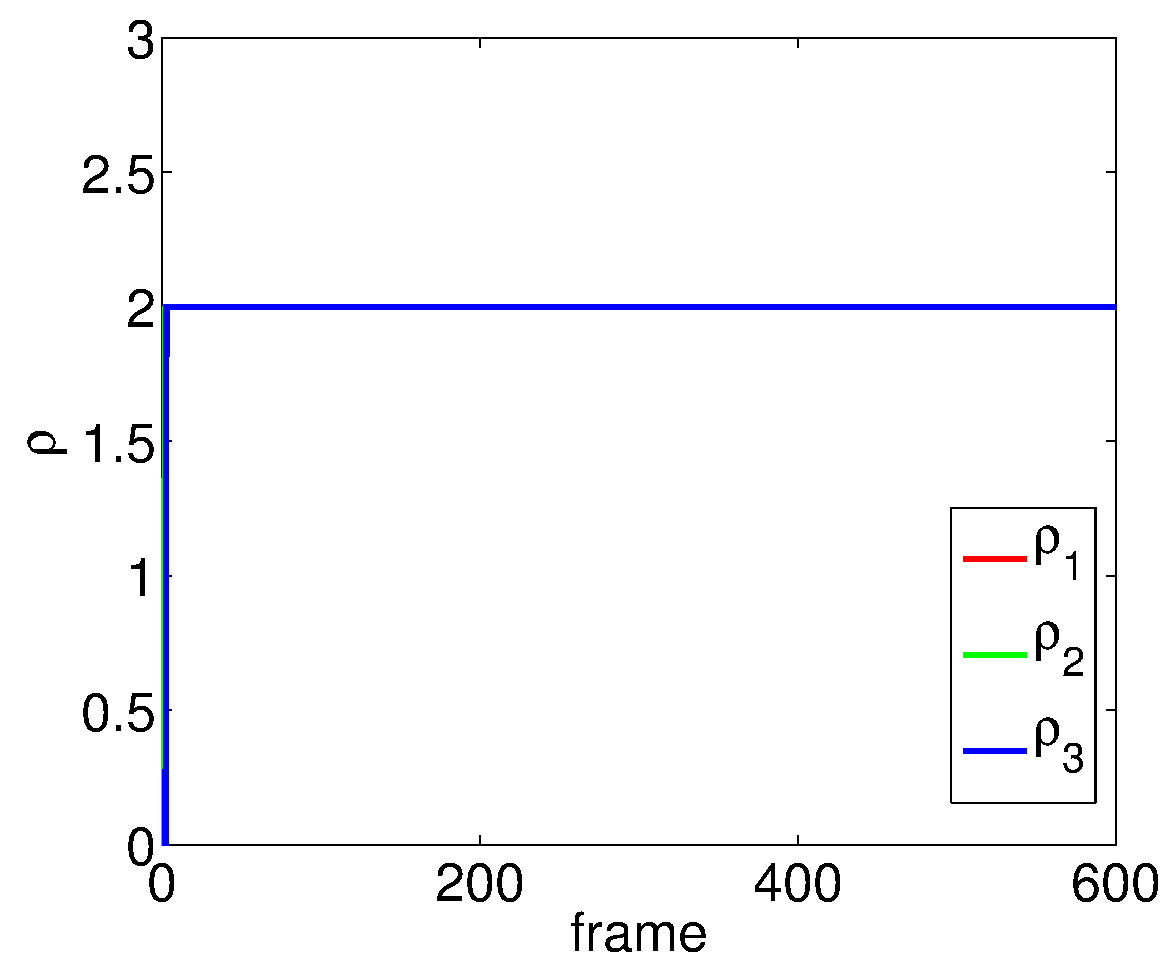
\includegraphics[width=0.45\textwidth]{figures/mcca_cca_corrs.pdf}
      }
      \subfigure[IMCCA Correlations]{
        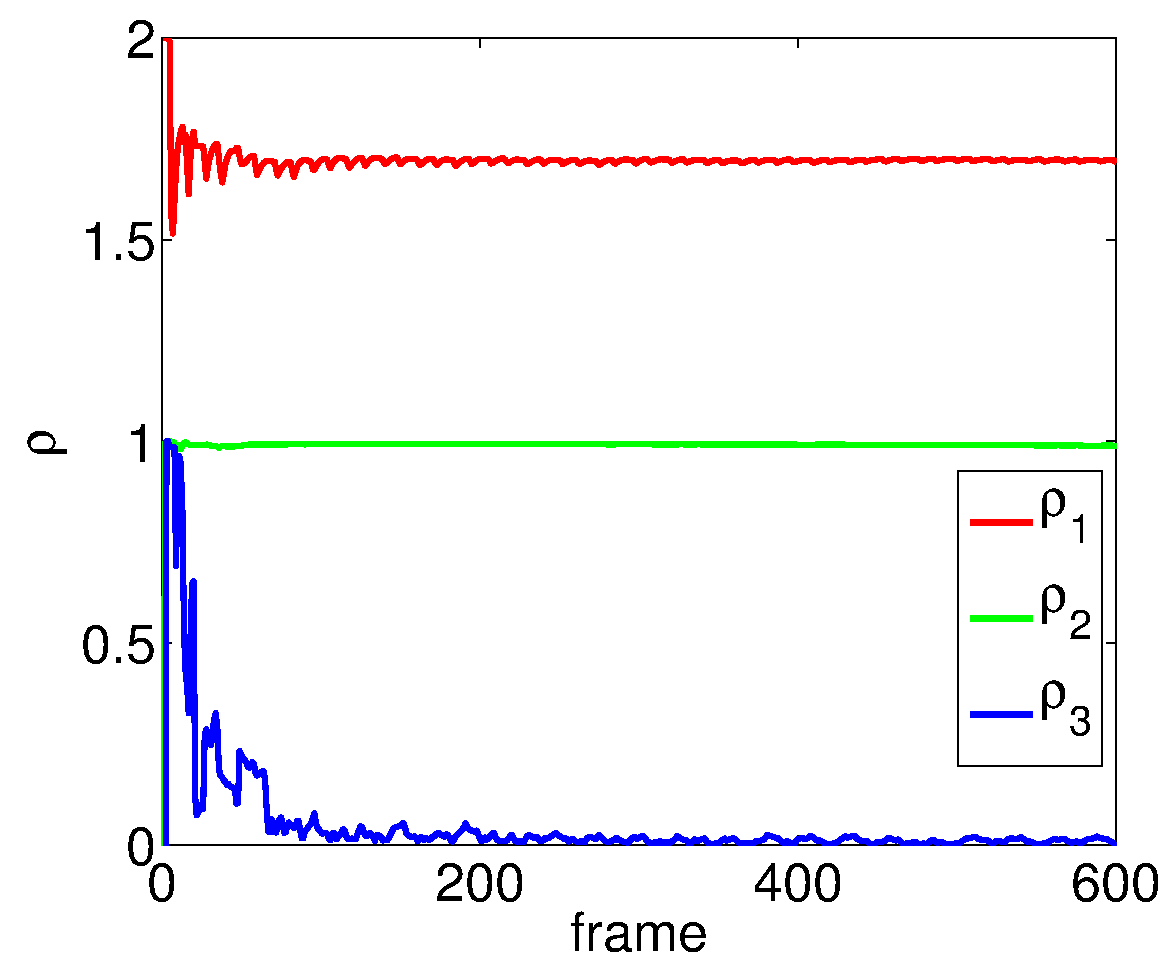
\includegraphics[width=0.45\textwidth]{figures/mcca_icca_corrs.pdf}
      }
    \end{center}
  \end{figure}
\end{frame}

\begin{frame}{Future Work}


\textbf{Kernel CCA}
\begin{itemize}
\item analysis for nonlinear low-rank signal-plus-noise model
\item analysis of choice of kernel
\item analysis of choice of regularization parameter
\end{itemize}

\vspace{2ex}

\textbf{MCCA}
\begin{itemize}
\item MAXVAR theorem for deterministic correlation when $n<\sum_i d_i$ 
\item null distribution for statistical test for number of correlated signals
\item consistency analysis for estimate of number of correlated signals
\end{itemize}

\vspace{2ex}

\textbf{Image Annotation and Retrieval}
\begin{itemize}
\item clever feature engineering with NLP techniques 
\item extension to nonlinear algorithms
\end{itemize}



\end{frame}

\begin{frame}{Acknowledgments}

\begin{itemize}
\item people i want to thank
\end{itemize}

\end{frame}


\end{document}
